\NeedsTeXFormat{LaTeX2e}[2005/12/01]
%%    2010/04/06 v1.0 Vorlage Master-Forschungspraktikum Versuchsauswertung
%%    based on the 2009/10/14 v0.1 GAUBM template by Prof Pruschke

\documentclass[twoside,        %% zweiseitiges Layout
               BCOR12mm,       %% Bindekorrektur 12 mm
% please comment out if report is in English
%               english,ngerman, %% Dokumentspr. Deutsch, Alternativspr. Englisch
% please remove comment if report is in English 
               ngerman,english, %% Dokumentspr. Englisch, Alternativspr. Deutsch
               fleqn,headsepline=false,footsepline=false
              ]{Vorlage/MFPREPORT}
\makeatletter
\DeclareOldFontCommand{\rm}{\normalfont\rmfamily}{\mathrm}
\DeclareOldFontCommand{\sf}{\normalfont\sffamily}{\mathsf}
\DeclareOldFontCommand{\tt}{\normalfont\ttfamily}{\mathtt}
\DeclareOldFontCommand{\bf}{\normalfont\bfseries}{\mathbf}
\DeclareOldFontCommand{\it}{\normalfont\itshape}{\mathit}
\DeclareOldFontCommand{\sl}{\normalfont\slshape}{\@nomath\sl}
\DeclareOldFontCommand{\sc}{\normalfont\scshape}{\@nomath\sc}
\makeatother

%% Pakete und Definitionen ausgelagert
\usepackage{a4}
\usepackage{multicol}

% language option set in JGNSUM class
\usepackage{babel}
\usepackage{hyperref}

%% FONT:
%\usepackage{lmodern}
\usepackage{times} % sieht besser aus als lmodern
%\usepackage{palatino} % sieht schlechter aus als times
%\usepackage{mathpazo} % very ugly font, to be loaded later ???
%\usepackage{cmbright} % doesn't work either
\usepackage[T1]{fontenc}
\usepackage{textcomp}

\usepackage{ucs}
\usepackage[utf8x]{inputenc}

\usepackage{amsfonts}
\usepackage{amstext}
\usepackage{amsmath}
\usepackage{amsthm}
\usepackage{amssymb}
\usepackage{amsbsy}   % AMS-Boldsymbol

% \usepackage{mathabx} % e.g. for \Sun
%% but not a standard package (neither texlive nor Miktex)
%% so use wasysym (\astrosun) instead
\usepackage{wasysym} % e.g. for \astrosun or \CheckedBox

\usepackage{bbm,mathrsfs}

\usepackage{textcomp} % noch einige coole symbole

\usepackage{sectsty}
\allsectionsfont{\raggedright}

\usepackage[numbers]{natbib}
\citestyle{dinat}
\bibliographystyle{dinat}

\usepackage{makeidx}

\usepackage{url}	% für hübsche URLs mit Link
\usepackage{color}	% für farben a la \definecolor{Gray}{gray}{0.5}
\usepackage{verbatim}
\usepackage{subfigure}
\usepackage{listings}

\usepackage{fancybox}
%usage:
%\begin{Verbatim}[frame=single,label=Titel]
%Verbatim Zeile
%\end{Verbatim}


 \setlength{\textwidth}{16.2cm}
 \setlength{\textheight}{24cm}
 \setlength{\oddsidemargin}{0cm}
 \setlength{\evensidemargin}{-0.5cm}

 %unbedingt nach abmessungen einfügen!
 \usepackage{fancyhdr}
 \pagestyle{fancy}
 %\sloppy % für weniger absatzfehler

 \setcounter{tocdepth}{2}
 \setcounter{secnumdepth}{2}

 \ifreportelse{\numberwithin{equation}{chapter}}{\numberwithin{equation}{section}}
 \theoremstyle{plain}% default
 \ifreportelse{\newtheorem{thm}{Theorem}[chapter]}{\newtheorem{thm}{Theorem}[section]}

 \newtheorem{satz}{Satz}
 \newtheorem{lem}[thm]{Lemma}
 \newtheorem{prop}[thm]{Proposition}
 \newtheorem{kor}[thm]{Korollar}
 \newtheorem{cor}[thm]{Corollary}

 \theoremstyle{definition}
 \newtheorem{defi}{Definition}

 \def\@proof{%
  \if@englishpreamble{Proof}\else{Beweis}\fi
 }
 \newenvironment{bew}{\begin{proof}[\@proof]}{\end{proof}}



%% einbinden einiger nützlicher Befehle
\newcommand{\iflanggerman}[2]{
 \iflanguage{german}{#1}{
  \iflanguage{ngerman}{#1}{#2}
 }
}

% box around the whole equation, number inclusive
\newcommand{\boxedeqn}[1]{%
  \[\fbox{%
      \addtolength{\linewidth}{-2\fboxsep}%
      \addtolength{\linewidth}{-2\fboxrule}%
      \begin{minipage}{\linewidth}%
      \begin{equation}#1\end{equation}%
      \end{minipage}%
    }\]%
}

\iflanggerman{
 \newcommand{\const}{\mathrm{konst}}
 \newcommand{\Const}{\mathrm{konst.}}
}{
 \newcommand{\const}{\mathrm{const}}
 \newcommand{\Const}{\mathrm{const.}}
}

% von Meier
\newcommand{\nbd}{\nobreakdash-\hspace{0pt}}
% example: $K$\nbd{}Vektorraum
\newcommand*{\transpose}[1]{\prescript{t}{}{#1}}
\newcommand*{\conjugate}[1]{\overline{#1}}
\newcommand*{\abs}[1]{\lvert#1\rvert}
\newcommand*{\Mod}{\mathrm{mod}}
\newcommand{\symdif}{\mathbin\triangle}
\DeclareMathOperator{\Graph}{Graph}
\DeclareMathOperator{\id}{id}
\DeclareMathOperator*{\grad}{grad}
\DeclareMathOperator*{\Div}{div}
\DeclareMathOperator*{\rot}{rot}
\DeclareMathOperator{\sig}{sig}
\DeclareMathOperator{\sgn}{sgn}
\DeclareMathOperator{\diag}{diag}
\DeclareMathOperator{\tr}{tr}
\DeclareMathOperator{\Sp}{Sp}
\DeclareMathOperator{\im}{Im}
\DeclareMathOperator{\re}{Re}

\newcommand{\vcentcolon}{\mathop{:}}



%Zur Formatierung in der Matheumgebung
\renewcommand{\t}{\ensuremath{\rm\tiny}} % Tiefgestellter Text in der Matheumgebung wird schoener mit: $\Phi_{\t{Text}}$
\renewcommand{\d}{\ensuremath{\mathrm{d}}} % Die totale Ableitung ist stets aufrecht zu setzen: \d
\newcommand{\diff}[3][]{\ensuremath{\frac{\d^{#1}#2}{\d#3^{#1}}}} % einfache Ableitung nach x: $\ddx{\Phi}$
\newcommand{\pdiff}[3][]{\ensuremath{\frac{\partial^{#1}#2}{\partial#3^{#1}}}} % wie gesprochen, eine partielle Ableitung: \del
\newcommand{\aeqiv}{\ensuremath{\qquad \Longleftrightarrow \qquad}} % Eine Aequivalenz
\newcommand{\folgt}{\ensuremath{\qquad \Longrightarrow \qquad}} % Ein Folgepfeil mit Abstaenden
\newcommand{\corresponds}{\ensuremath{\mathrel{\widehat{=}}}} % Befehl für "Entspricht"-Zeichen
\newcommand{\mi}[1]{\ensuremath{\mathit{#1}}} % italics für griechische Buchstaben in Matheumgebung

%Um nicht so viel schreiben zu müssen...
\newcommand{\bs}[1]{\boldsymbol{#1}}
\newcommand{\ol}[1]{\overline{#1}}
\newcommand{\wtilde}[1]{\widetilde{#1}}
\newcommand{\mrm}[1]{\mathrm{#1}}
\newcommand{\mbf}[1]{\mathbf{#1}}
\newcommand{\mbb}[1]{\mathbb{#1}}
\newcommand{\mcal}[1]{\mathcal{#1}}
\newcommand{\mfrak}[1]{\mathfrak{#1}}

%Abkürzungen
\newcommand{\zB}{z.\,B.\ }
\newcommand{\bzw}{b.\,z.\, w.\ }
\newcommand{\Dh}{d.\,h.\ }
\newcommand{\Gl}{Gl.\ }
\newcommand{\Abb}{Abb.\ }
\newcommand{\Tab}{Tab.\ }

\usepackage{braket}
\usepackage{cleveref}
\usepackage{graphicx, subfigure}
\usepackage{rotating}
\usepackage{appendix}


\begin{document}
\LabratoryName{KT.WZE}{W/Z experiment at the Tevatron}
\ProtocolAuthor{Eric}{Bertok}{eric.bertok@stud.uni-goettingen.de}
\Assistant{Dr. J. Veatch}{}
\ResearchFocus{Nuclear and particle physics (M.phy.404)}
\ConductedOn{24}{01}{2018}
\date{\today}
% eines von beiden
\CopyNotWanted
%\CopyWanted

\pagenumbering{roman}
\maketitle

%\begin{otherlanguage}{english}
%\end{otherlanguage}

\tableofcontents

\clearpage
\pagenumbering{arabic}

\section{Introduction}
\label{sec:introduction}
The goal of this experiment is the determination the  of the branching ratio of the $W$ boson
BR($W\rightarrow\mu\nu$). First, $W$ and $Z$ bosons are reconstructed using
data provided by the Tevatron collider at Fermilab. By comparing with monte-carlo
simulations, selection parameters are obtained, which allow for clean cuts for
filtering out background events (jets and cosmic source). The mass and the
transverse mass is then determined for the $Z$ and $W$ boson respectively.
Finally the branching ratio is calculated from the number of selected events,
the trigger efficiencies, as well as the reconstruction efficiencies.


\section{Theory}
\label{sec:theory}
\subsection{Electroweak interaction}
The GWS theory (Glashow, Weinberg, Salam) is the unified description of both
the electromagnetic force mediated by the photon and the weak interaction
mediated by the massive $W^+,W^-$ and the neutral neutral $Z$ boson. It was
confirmed experimentally in the 1970s \cite{wikigsw}. 
The gauge bosons are introduced by means of a local SU(2)$_L$ gauge symmetry in
a weak isospin space. The weak isospin doublets are formed by fermions
differing by one unit of charge \cite[p.;416]{thomson}. By also replacing the
U(1) symmetry by a new U(1)$_Y$ symmetry with the ``hypercharge'' $Y$, the
neutral $Z$ boson can be identified by a linear combination of the neutral
$W^{(3)}$ boson and the $B$ boson coupling to the hypercharge. More details can
be found in \cite[p.\;418ff]{thomson}.
Being a charged boson,
the $W$ bosons couple to fermions differing by one unit of charge. Furthermore
it maximally violates parity as it only couples to left-handed particles and
right-handed antiparticles. The vertex factor is given by \cite[p.;409]{thomson}
\begin{align}
    \label{eq:vertexw}
    -i\frac{g_W}{\sqrt{2}}\frac{1}{2}\gamma^\mu(1-\gamma^5),
\end{align} where $g_W$ is the weak coupling constant and $\gamma^\mu$ are the
gamma matrices. The $Z$ boson however, couples to any pair of identical
fermions, albeit coupling more strongly to left handed ones. This becomes
apparent in the form of the vertex factor: \cite[p.\;432]{thomson}
\begin{align}
    \label{eq:vertexz}
    -i\frac{1}{2}g_Z \gamma^\mu(c_V-c_A\gamma^5),
\end{align}
with the vector and axial vector couplings $c_V$ and $c_A$.

\subsection{Matrix elements and Decay rates}
The matrix elements for the electroweak interaction can be calculated with the
appropriate Feynman rules.
After averaging over the three possible polarizations, the spin-averaged matrix
element squared is obtained for both the $W$ and the $Z$ boson decaying to a
lepton and its neutrino or a lepton- anti-lepton pair, respectively
\cite[p.;242,411]{thomson}:
\begin{align}
    \label{eq:spinavg}
    \braket{|\mathcal{M}_W^2|}&=\frac{1}{3}g_W^2m_W^2\\
    \braket{|\mathcal{M}_Z^2|}&=\frac{1}{3}(c_V^2+c_A^2)g_Z^2m_Z^2.
\end{align}
These can be inserted into the decay rate formula: \cite[p.\;411]{thomson}
\begin{align}
    \label{eq:decayrate}
    \Gamma=\frac{p^*}{32\pi^2m^2}\int
    \braket{|\mathcal{M}^2|}\d\Omega=\frac{p^*}{8\pi m^2}
    \braket{|\mathcal{M}^2|},
\end{align}
where $m$ is the mass of the boson and $p*$ is the momentum of the lepton in
the center of mass frame.
One can argue that $p*=m_Z/2$, as the
decay happens in the centre of mass frame of the decaying particle.
Therefore the decay rate is 
\begin{align}
    \label{eq:decay}
    \Gamma(W^-\rightarrow e^- \bar{\nu}_e)&=\frac{g_W^2m_W}{48\pi}.\\
    \Gamma(Z\rightarrow e^- e^+)&=\frac{g_Z^2m_Z}{48\pi}(c_V^2+c_A^2).
\end{align}
Lepton universality tells us that this is the same for all three leptonic
channels when neglecting masses. For hadronic processes, the CKM matrix has to
be considered, while excluding the top quark, as it is too massive.
For the $W$ boson, one obtains for the decay width \cite{thomson} 
\begin{align}
\Gamma_W=(3+6 \kappa)\Gamma(W^-\rightarrow e^-
\bar\nu_e)\approx9.2\;\frac{g_W^2m_W}{48\pi}=2.1\;\text{GeV.}
    \label{eq:gammaw}
\end{align}
$\kappa\approx1.038$ is a correction factor that accounts for second order QCD processes.
Similarly, for the $Z$ boson, one obtains
\begin{align}
    \Gamma_Z\approx2.5\;\text{GeV.}    \label{eq:gammaZ}
\end{align}
The branching ratios for the muon channel are therefore
\begin{align}
    BR(W\rightarrow\mu\bar\nu_\mu)&=10.8\%,\\
    BR(Z\rightarrow\mu^+\mu^-)&=3.5\%.
    \label{eq:branches}
\end{align}
\subsection{Invariant and transverse mass}
For the $Z$ boson one can calculate the functional form of the invariant mass
peak by taking into account its finite lifetime.
The cross section for a $q\bar q\rightarrow \mu^+\mu^-$ event is proportional
to \cite{thomson} 
\begin{align}
    \sigma\propto|\mathcal{M}|^2\propto\left|\frac{1}{q^2-m_Z^2+im_Z\Gamma_Z}\right|^2=\frac{1}{(q^2-m_Z^2)^2+m_Z^2\Gamma_Z^2},
    \label{eq:breit}
\end{align}which is a Breit-Wigner curve.
$q$ is the invariant mass of both muons. As both can be detected in such an
event, the Breit-Wigner-curve can be fitted directly to the selected data to
obtain the mass of the $Z$ boson.
For the $W$ boson, things are more complicated. Due to the $W$ events only
having one muon, the undetectable neutrino has to be reconstructed from the
missing momentum. For a hadron collider such as the tevatron, the total
centre of mass energy cannot be known on an event to event basis due to
the composite nature of the hadrons. More specifically, the $z$-momentum of the
interacting partons are unknown, making the invariant mass reconstruction
impossible. However, one can define the transverse mass $M_T$, which can be
calculated from the reconstructed transverse momentum of the neutrino
$\bold{p}_T^\mu$. First, the missing transverse energy $MET$ is determined as
\begin{align}
    MET\approx|\bold{p}_T^\nu=|-\bold{p}_T^\mu-\bold{u}_T,
    \label{eq:met}
\end{align}where $\bold{u}_T$ is the transverse momentum of the hadrons
\cite{thomson}.
The transverse mass is then defined as
\begin{align}
    M_T=\sqrt{(MET+\bold{p}_T^\mu)^2-(MET_x+p_x^\mu)^2-(MET_y+p_y^\mu)^2}.
    \label{eq:mt}
\end{align}
This quantity is lorentz invariant but does not peak at $m_Z$. However, the $W$
mass can be read off from the position of the dropoff, as the longitudinal
component of the invariant mass is then close to zero.


\section{Experimental setup and methods}
\label{sec:setup}
For this experiment, two types of data have been provided: The first is a subset

of real data from the D\O\;detector at Fermilab near Chicago. The second are two
sets of simulated monte-carlo W and Z events generated by PYTHIA
\cite{pythia}.\\
At the D\O\; detector, muons are identified  both in the muon detector and the
tracking system. Whereas the tracking system directly surrounds the interaction
point and allows for gauging the muon's momentum and direction precisely, the
outer muon detector is mostly used to match the track in the tracking system.
This is possible because muons are the only particles capable of reaching the
muon detector, due to a combination of their relatively long lifetime and small calorimeter energy deposition. For more details on the D\O\;  detector see
\cite{d0}.
As the sheer amount of data from the collider is too much to analyse and save,
both software and hardware triggers are used to decide, whether an event is
worth investigating. The data that is provided is pre-filtered for at least one
muon in every event that has a transverse momentum of at least 15\;GeV/c.
The monte-carlo data has been reconstructed, such that the
events look like real data. Therefore the monte-carlo serves a benchmark for
the analysis of the real data.
To obtain invariant mass peaks for the $Z$- as well as the transverse mass peak
for the $W$ boson, the right events have to be selected out of the ~3 million
events provided. This happens by first fixing a set of object level cuts, which
define what is counted as a muon. These cuts are the same for both $W$- and $Z$ boson analysis
. Secondly, a range of object level cuts have to be performed to single
out the right events for $Z$ and $W$ production respectively. These have to be
physically motivated by keeping in mind what is expected for the muons in a
$W$ or $Z$ decay and should also be compared to the monte-carlo simulation. By
first comparing various muon parameters for the simulated data and the uncut
experimental data, one can define appropriate cuts in these parameters that cut
out most events not present in the simulation while also keeping events that do
resemble the simulation mostly intact. Finally the real data is plotted with
these cuts performed and compared with the simulated results. This process is
repeated until a satisfactory isolation of $Z$ or $W$ events has been produced.
All of the analysis is done with ROOT \cite{root}.

\section{Analysis}
\label{sec:analysis}
\subsection{Selection of $Z \rightarrow \mu\mu$ events}
The $Z$ boson mass distribution for the simulated monte-carlo data is shown in
\cref{fig:zmcmass}.
\begin{figure}
    \subfigure[]{
        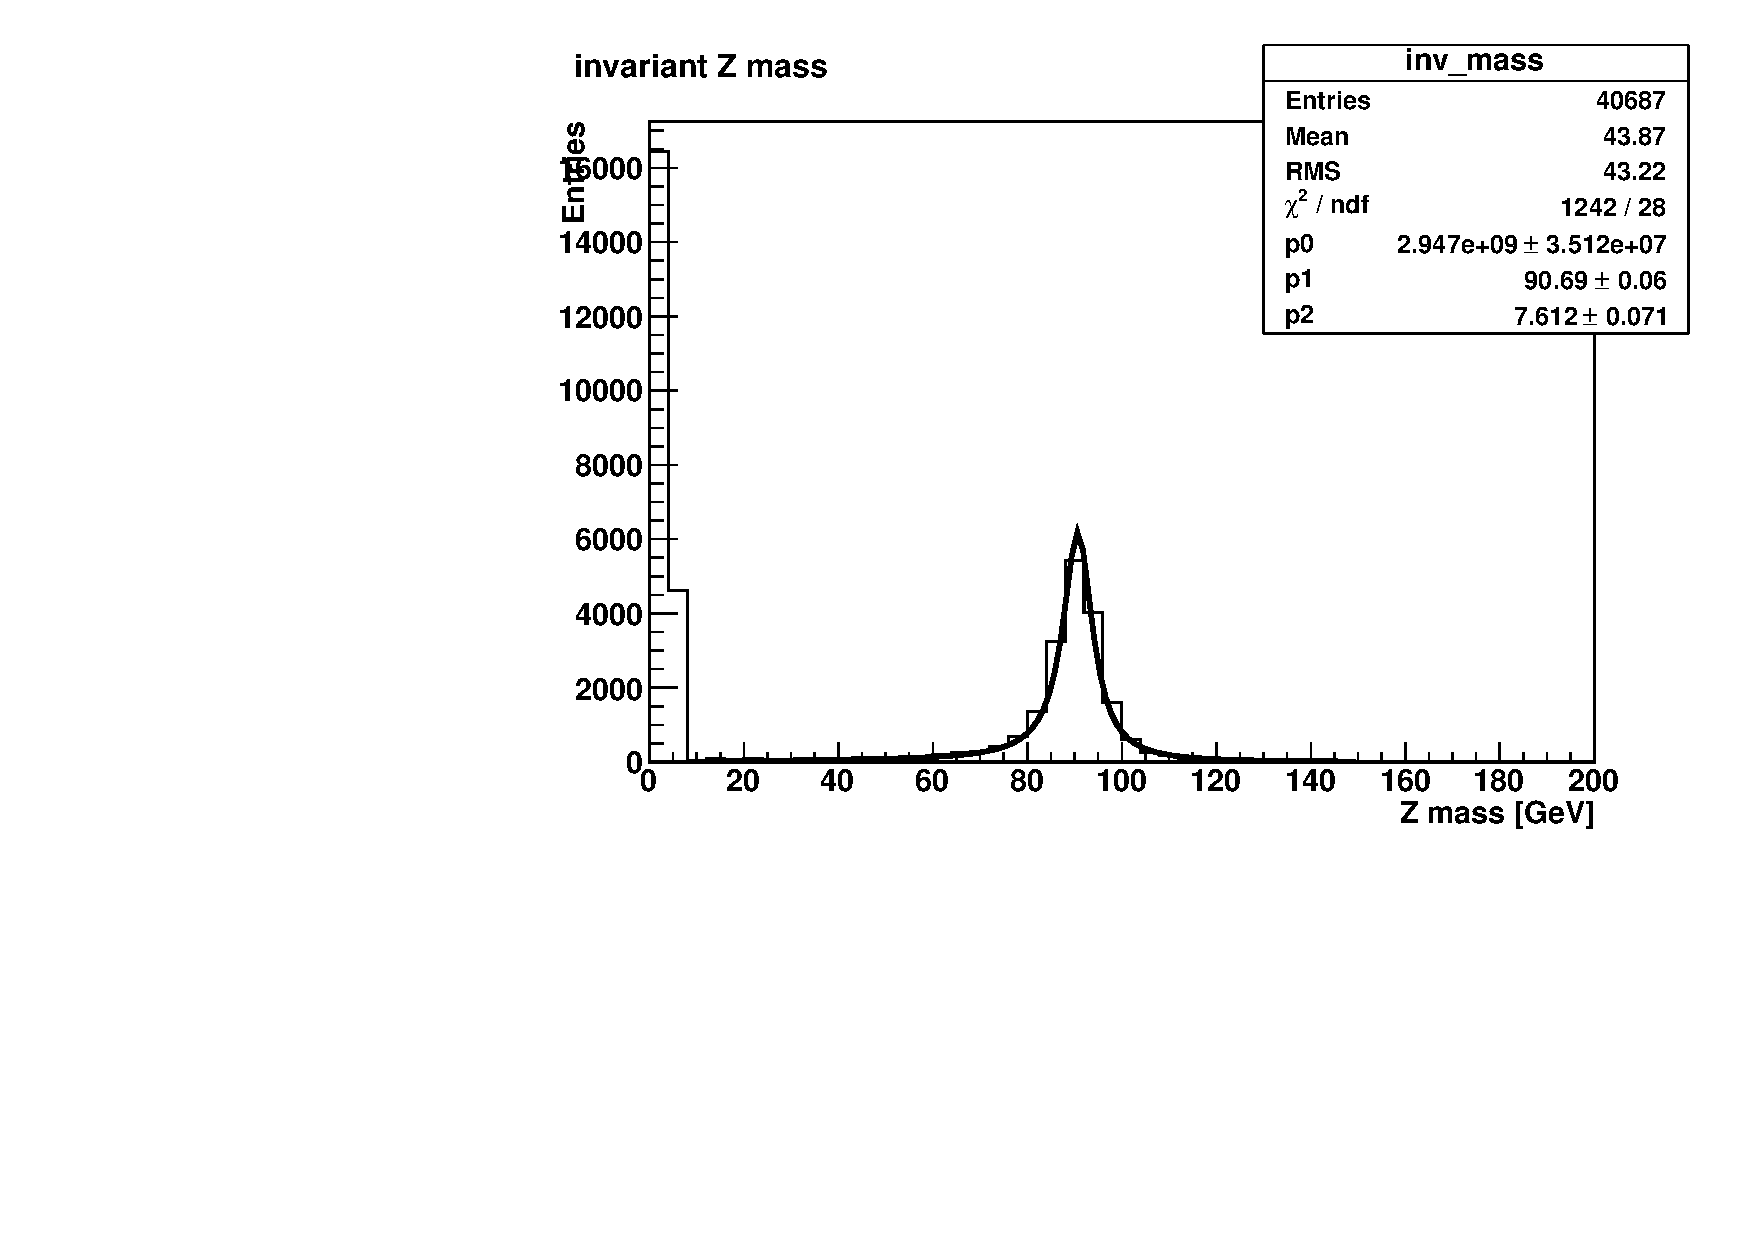
\includegraphics[width=0.45\textwidth]{fig/zmc_uncut_zmass.pdf}
        \label{fig:zmcmass}
    }
    \subfigure[]{
        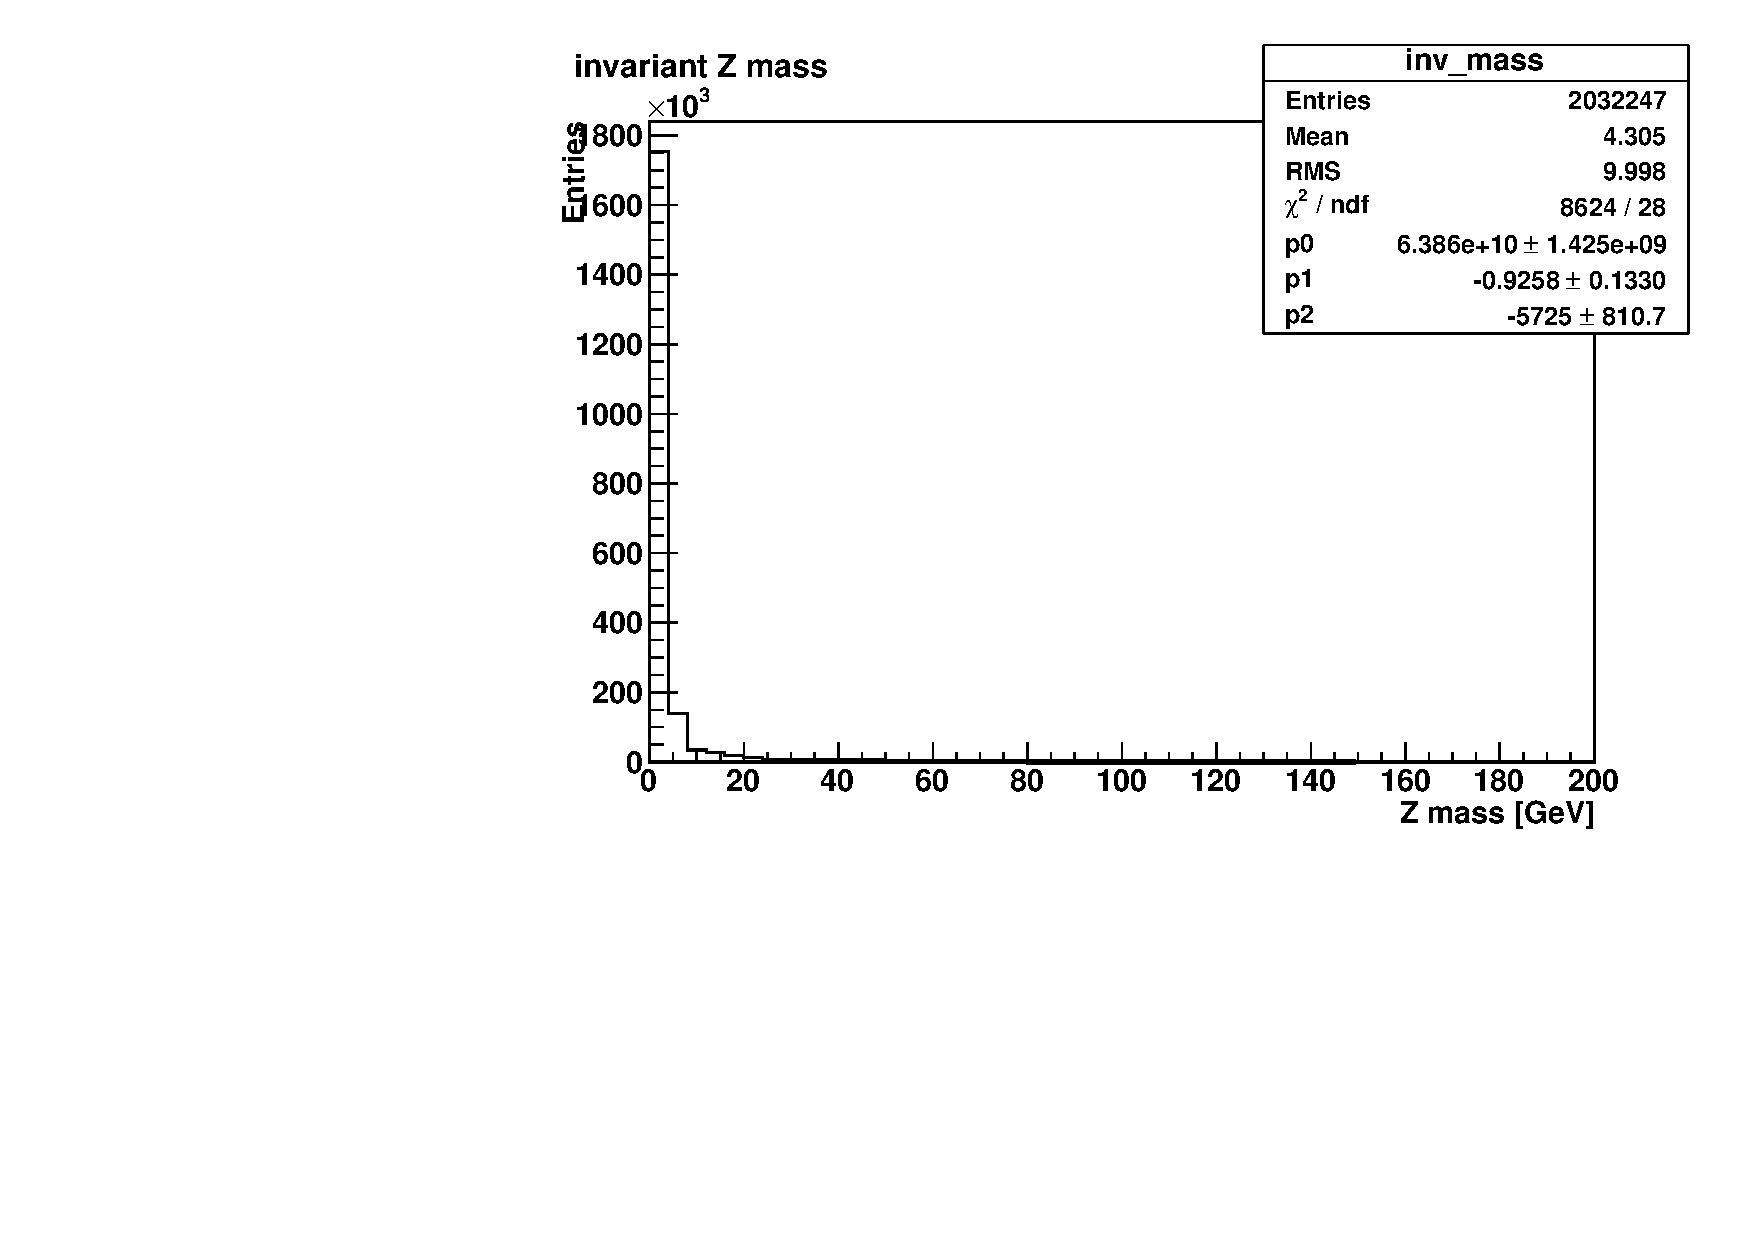
\includegraphics[width=0.45\textwidth]{fig/data_uncut_zmass.pdf}
        \label{fig:uncutZmass}
    }
    \caption{$Z$ mass plotted for both monte-carlo (left) and real data (right)
    without any cuts. One can clearly see the expected mass peak at the monte
    carlo case, as well as a leage number of events with very low mass, while in
    the real data plot, no mass peak is visible yet. For the monte-carlo case,
    a $\chi^2$ fit is performed with the Breit-Wigner curve.}
\end{figure}
One can clearly see the mass peak of the Z boson. A large number of events,
however, is also situated at the beginning of the mass spectrum. A fit
performed by root with the function \ref{eq:breit}
\begin{align}
    \sigma\propto\frac{1}{(q^2-m_Z^2)^2+m_Z^2\Gamma_Z^2}
    \label{eq:breit}
\end{align}
is performed, with the parameters $p_0$ as a constant proportionality factor,
$p_1$ being $m_Z$ and $p_2$ being the decay width $\Gamma$. The results are
summarized together with all other fits in \cref{tab:fits}.
Apart from the large number of events at low mass, this clearly resembles the
expected $Z$ mass peak. In \cref{fig:uncutZmass}, the uncut real data is
plotted. From the ~2 million events, almost all of them give a very small $Z$
mass and the peak is not visible. Note that the trigger
``TRIG\_MUW\_W\_L2M3\_TRK10'' \cite{fprakt} is still included in the uncut case.
Additional object level cuts are performed, which are summarized in
\cref{tab:objectcuts}. These are identical for both $Z$ and $W$ boson analysis
as they will effectively cancel out when calculating the efficiencies.
The accepted and rejected events for both $Z$ monte-carlo and real data are
shown in \cref{app:z} (\cref{fig:pt,fig:chi,fig:ehalo}).
To further separate background events, event level cuts are performed. Firstly,
events where only one muon are detected are rejected, as in a $Z$ decay, two
muons are expected. Secondly, both muons should have different charge due to
conservation of charge. Two muons with same charge indicate either two seperate
processes both creating a positively / negatively charged muon or a cosmic
event in which one cosmic muon crosses both detectors.


\begin{table}
    \centering
    \begin{tabular}{|c|c|c|}\hline
        parameter&condition&desription\\\hline
        $p_{T_1}$&$>20$&transverse momentum of the first muon in the central
        tracker\\\hline
        $p_{T_2}$&$>15$&transverse momentum of the second muon in the central
        tracker \\\hline
        $\chi_{1/2}^2$&$<2$&Chi squared per d.o.f. for the track fit\\\hline
        $E_{\text{halo}_{1/2}}$&$< 1.5$&transverse calorimeter energy in an
        annulus of $0.1 < R < 0.4$ around the muon\\\hline
    \end{tabular}
    \caption{Additional object level cuts for the muons for both $Z$ and $W$
    analysis.}
    \label{tab:objectcuts}
\end{table}

\subsection{Cosmics}
The cosmic-ray background stems from high energy cosmic particles entering the
earth's atmosphere, where they decay into jets of particles. Muons are also
created this way. Because of time dilation, they can reach the earth's surface
before they decay, leading to the cosmic background in the detector.
In order to identify cosmic events, both timing and angular seperation are
taken into account. First, it is expected that timing differences from muons
originating from $Z$ decays have a negligible time difference at both muon
detectors, since the $Z$ boson can be treated as stationary in the lab frame.
Cosmic muons, however, should be detected at one side of the detector first and
at a later time on the other side, since they need to travel the distance of
the detector first. The timing difference for $Z$ monte-carlo and real data is
plotted in \cref{fig:timing}. A maximal time difference of $\Delta t=10$\;ns
was chosen as cut condition. However, also the simulated data shows two peaks
at around $100$\;ns.
Next, a two-dimensional histogram is plotted with the angular seperation
$\Delta\eta$ and $\Delta\phi$ as parameters. $\eta$ is the pseudorapidity of the
track and gives a measure of the tilt from the beam axis, while $\phi$  is the
angle around the beam axis. The result is shown for the simulation and real
data in \cref{fig:angle}. Note that so far, no angular cuts have been performed
at all. Still, with the cuts given above, there is a clear preference for
$\Delta\phi=\pi$ for both simulation and real data. This is desired, as this
means that the $Z$ boson upon its decay is quasi-stationary and therefore both
muons produced in the decay travel in opposite directions, as expected from
momentum conservation. Therefore, a decision was made not to perform any more
cuts containing angular information. As will be seen below, the cuts performed
thus-far give a very satisfactory result for the reconstructed $Z$ mass peak.
The reason for this will be discussed in \cref{sec:discussion}.
\begin{figure}
     \begin{center}
         \subfigure[]{
            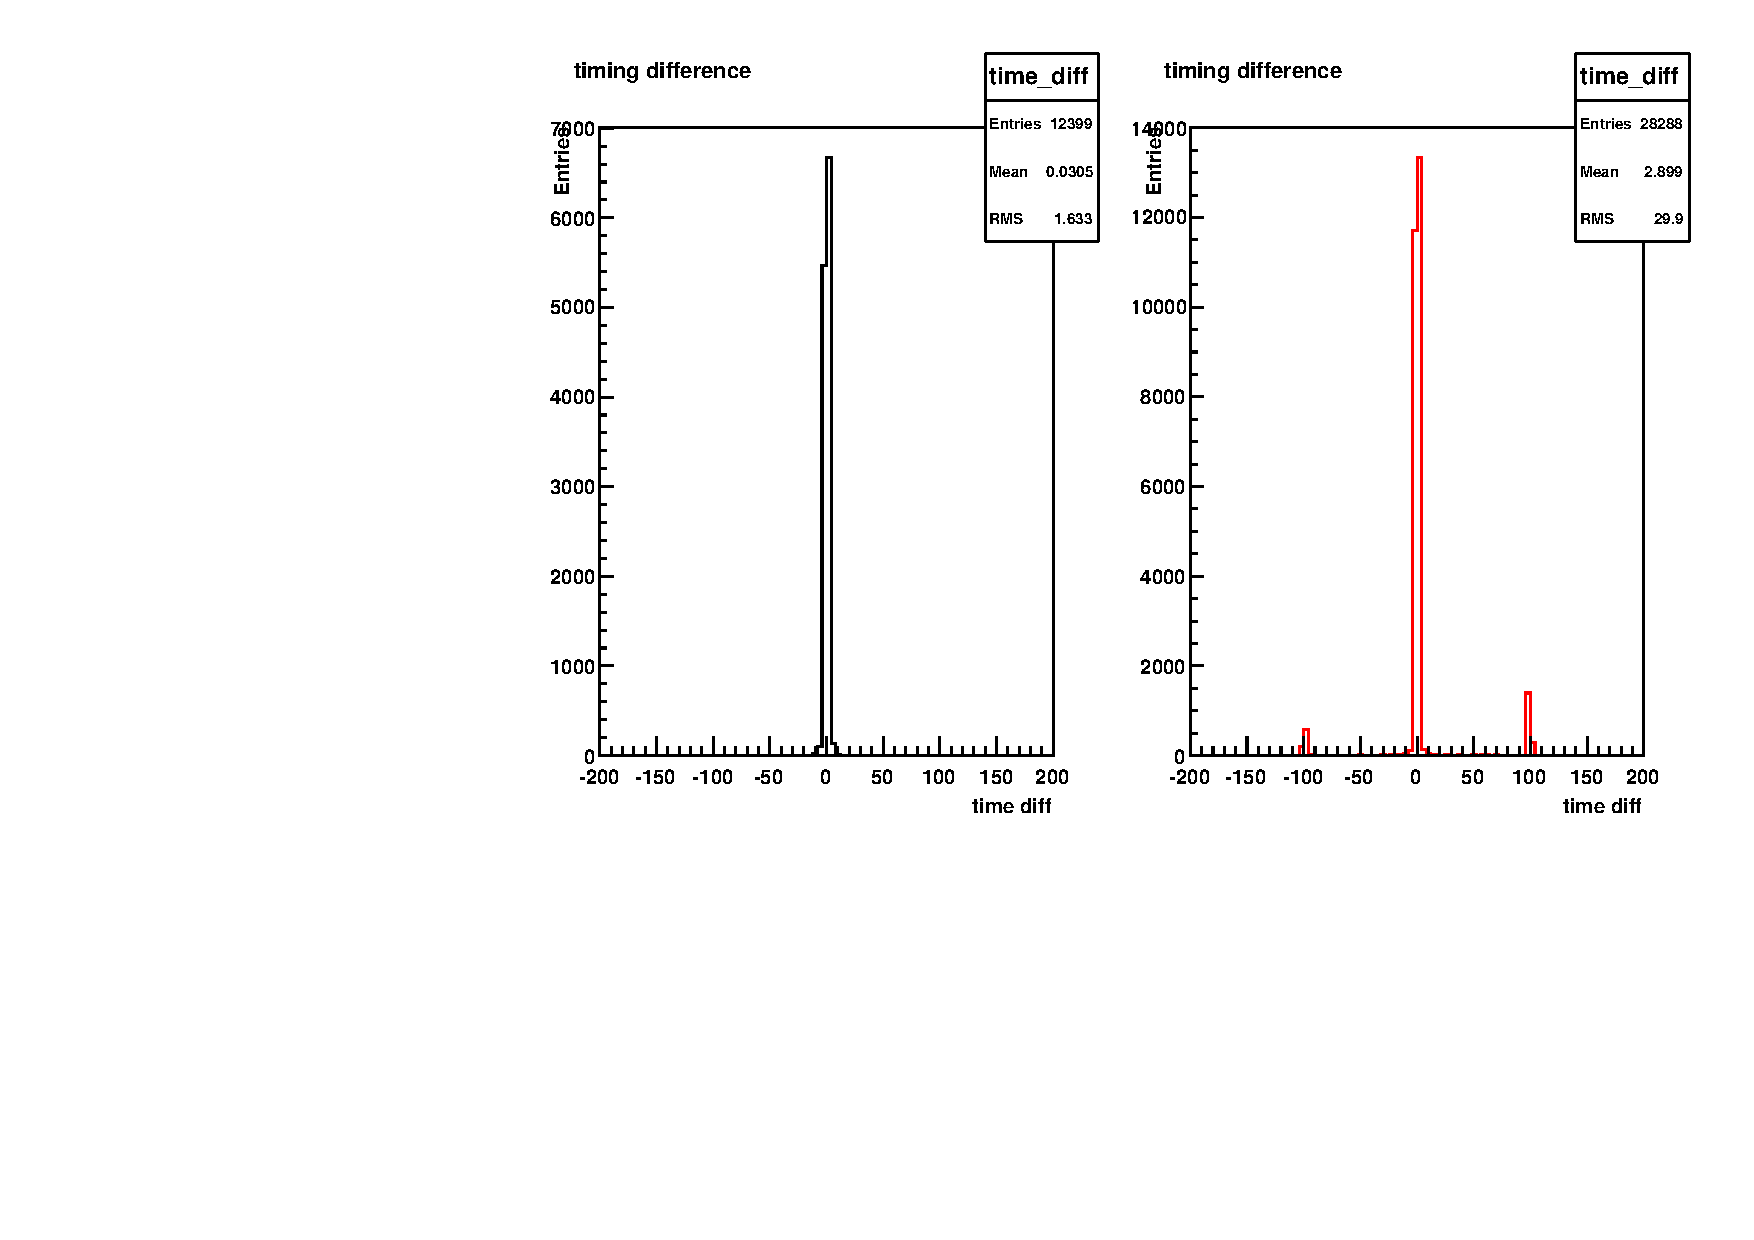
\includegraphics[width=0.8\textwidth,height=6 cm]{fig/zmc_cut_timediff.pdf}
        }\\ %  ------- End of the first row ----------------------%
        \subfigure[]{
            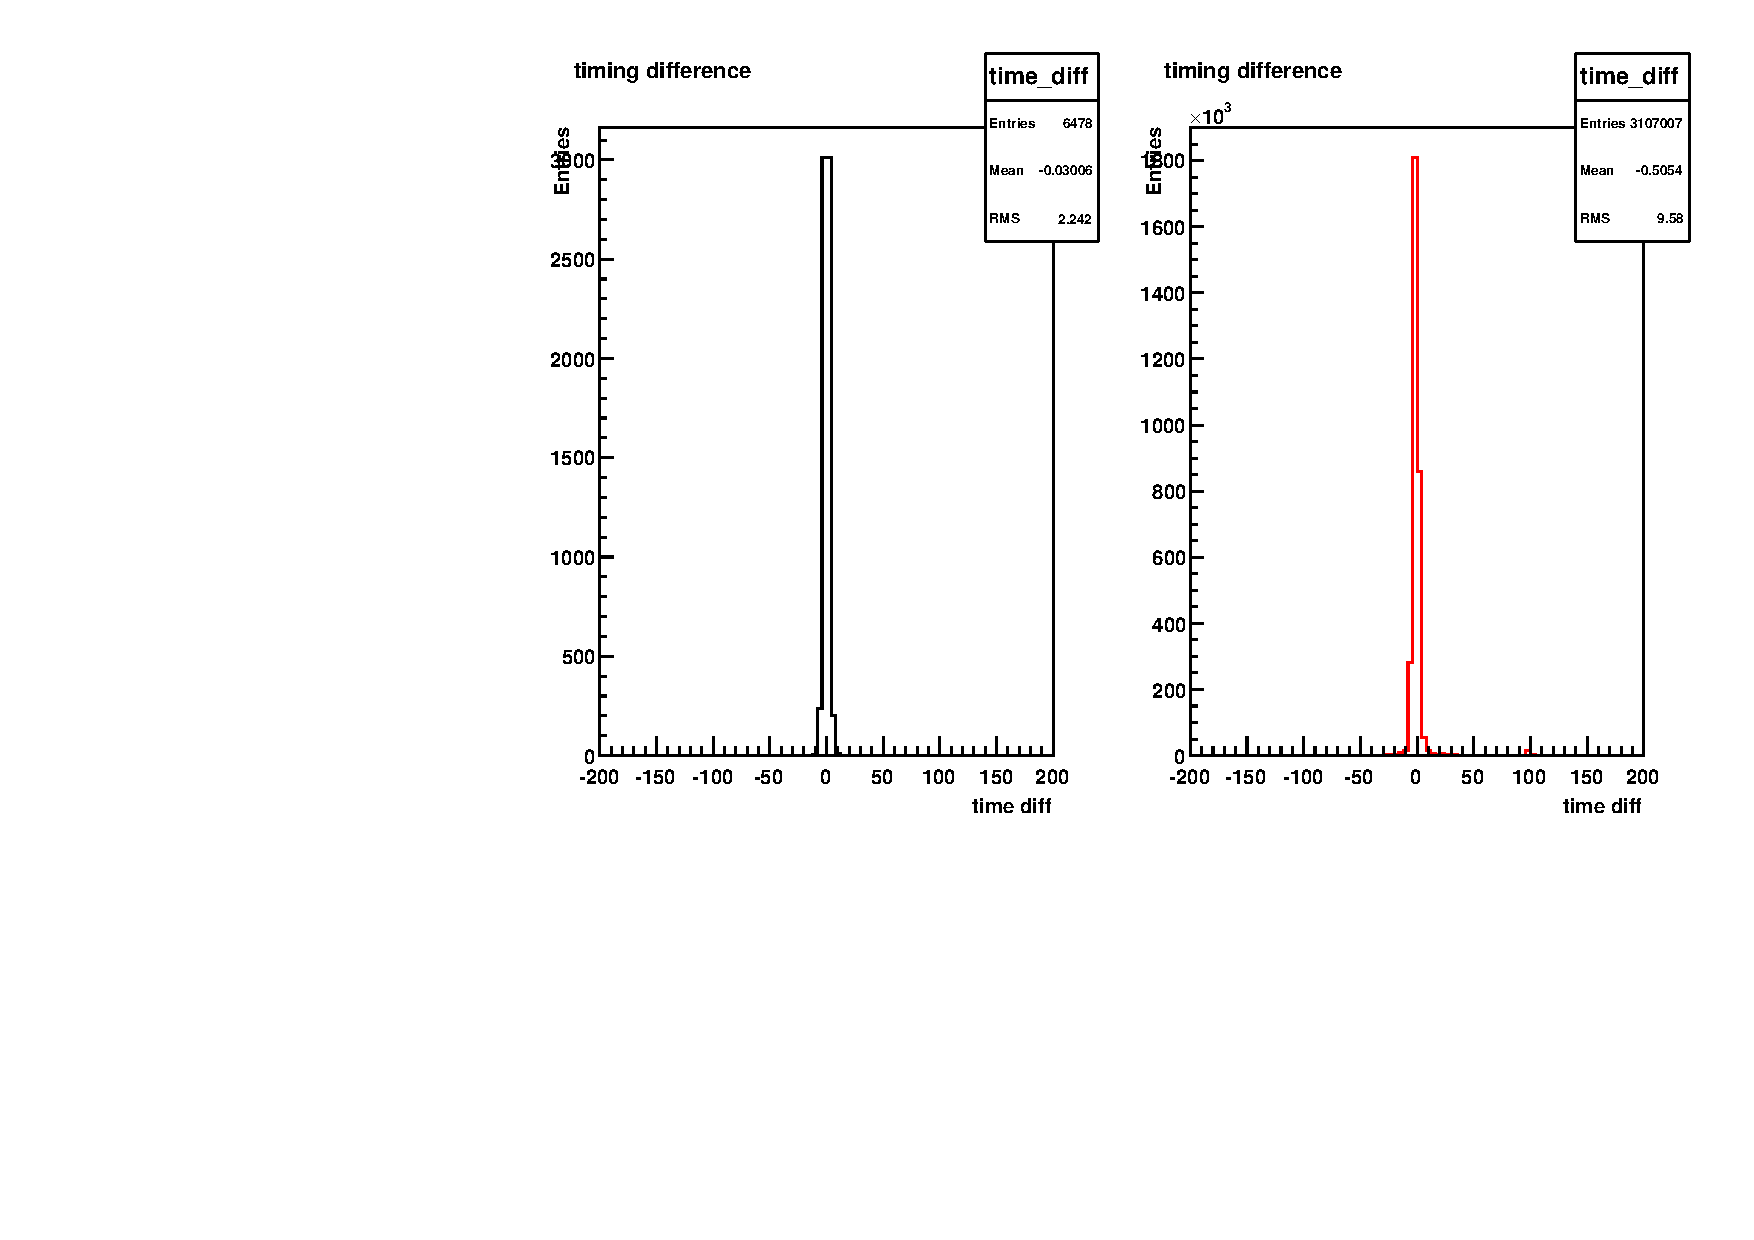
\includegraphics[width=0.8\textwidth,height=6 cm]{fig/data_cut_timediff.pdf}
        }
    \end{center}
    \caption{Timing difference between the first and second muon detection for
    the $Z$ monte-carlo (a) and the real data (b) in ns. On the right: rejected
events. On the left: accepted events.}
   \label{fig:timing}
\end{figure}
\begin{figure}
     \begin{center}
         \subfigure[]{
            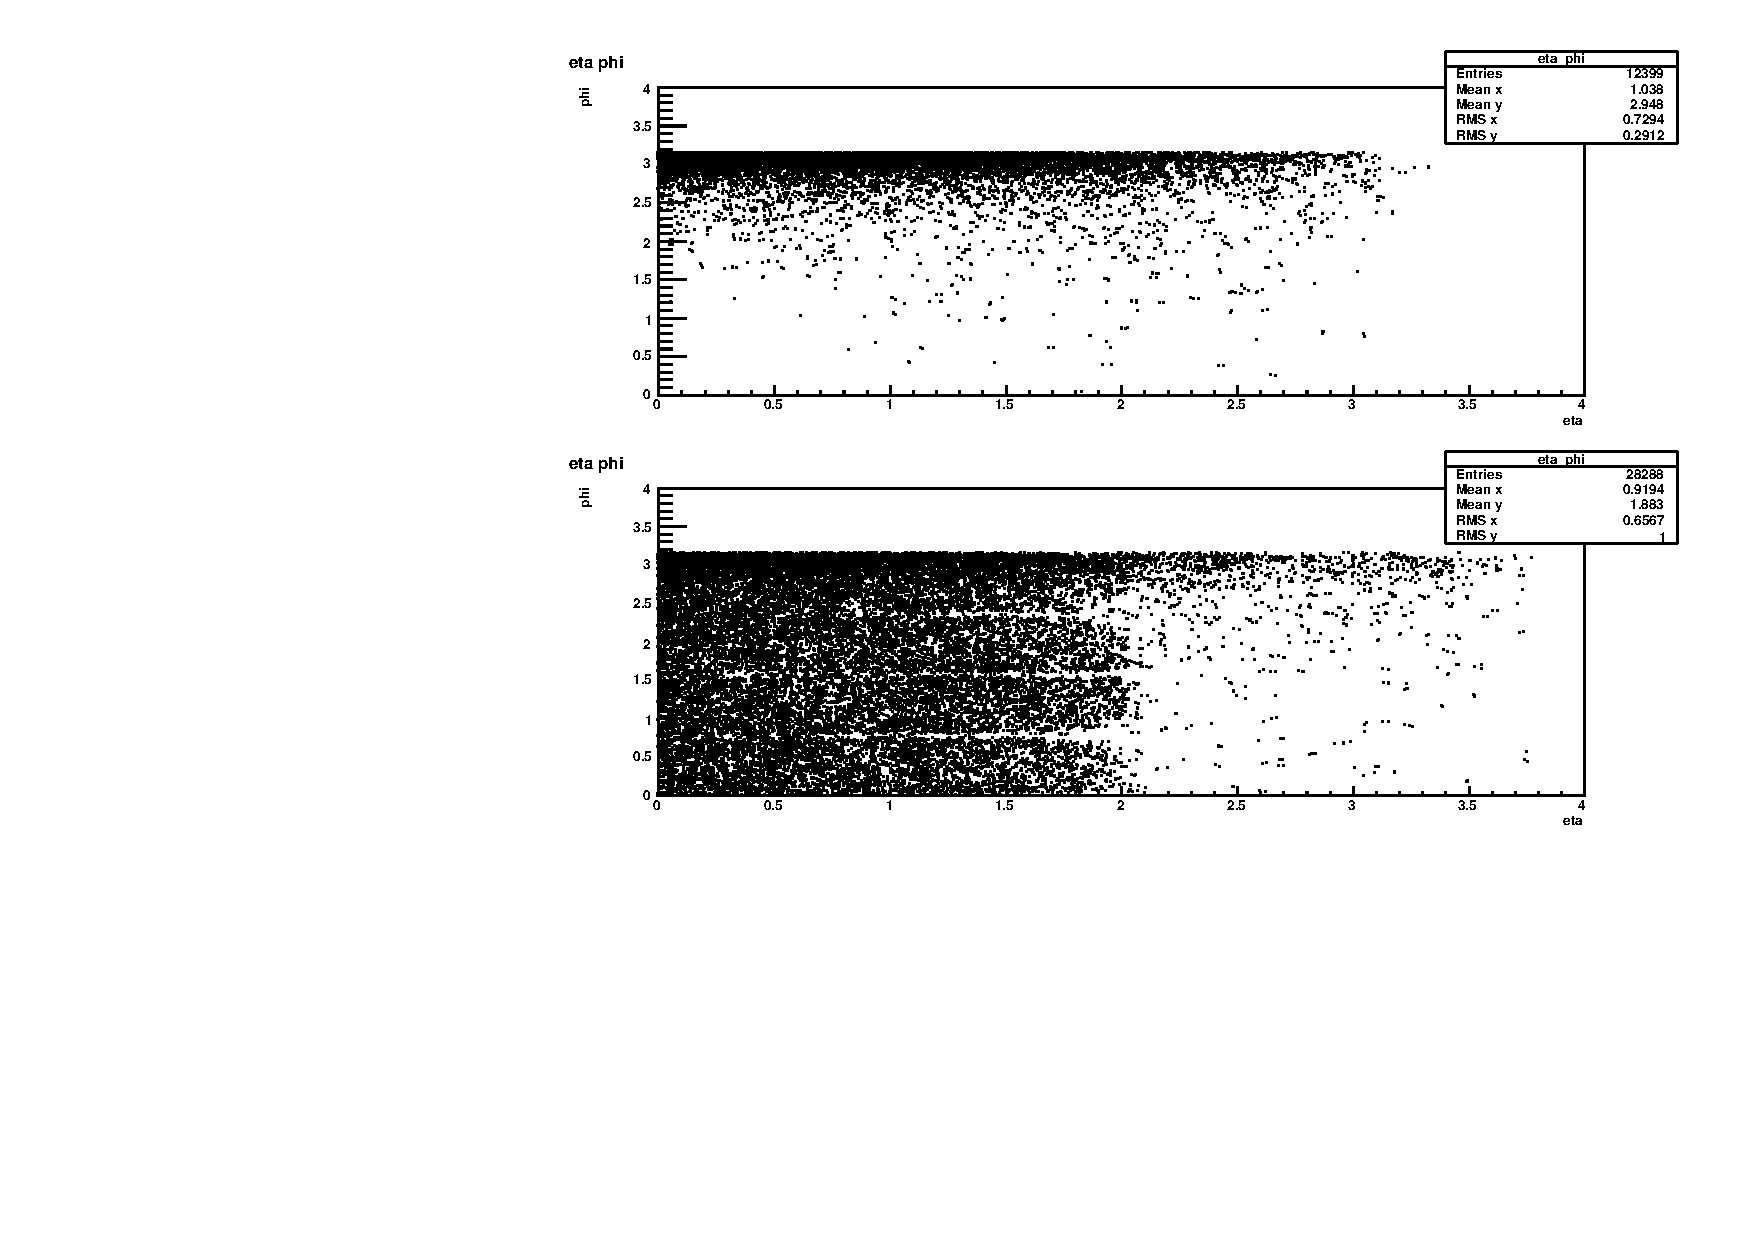
\includegraphics[width=0.9\textwidth]{fig/zmc_cut_etaphi.pdf}
        }\\ %  ------- End of the first row ----------------------%
        \subfigure[]{
            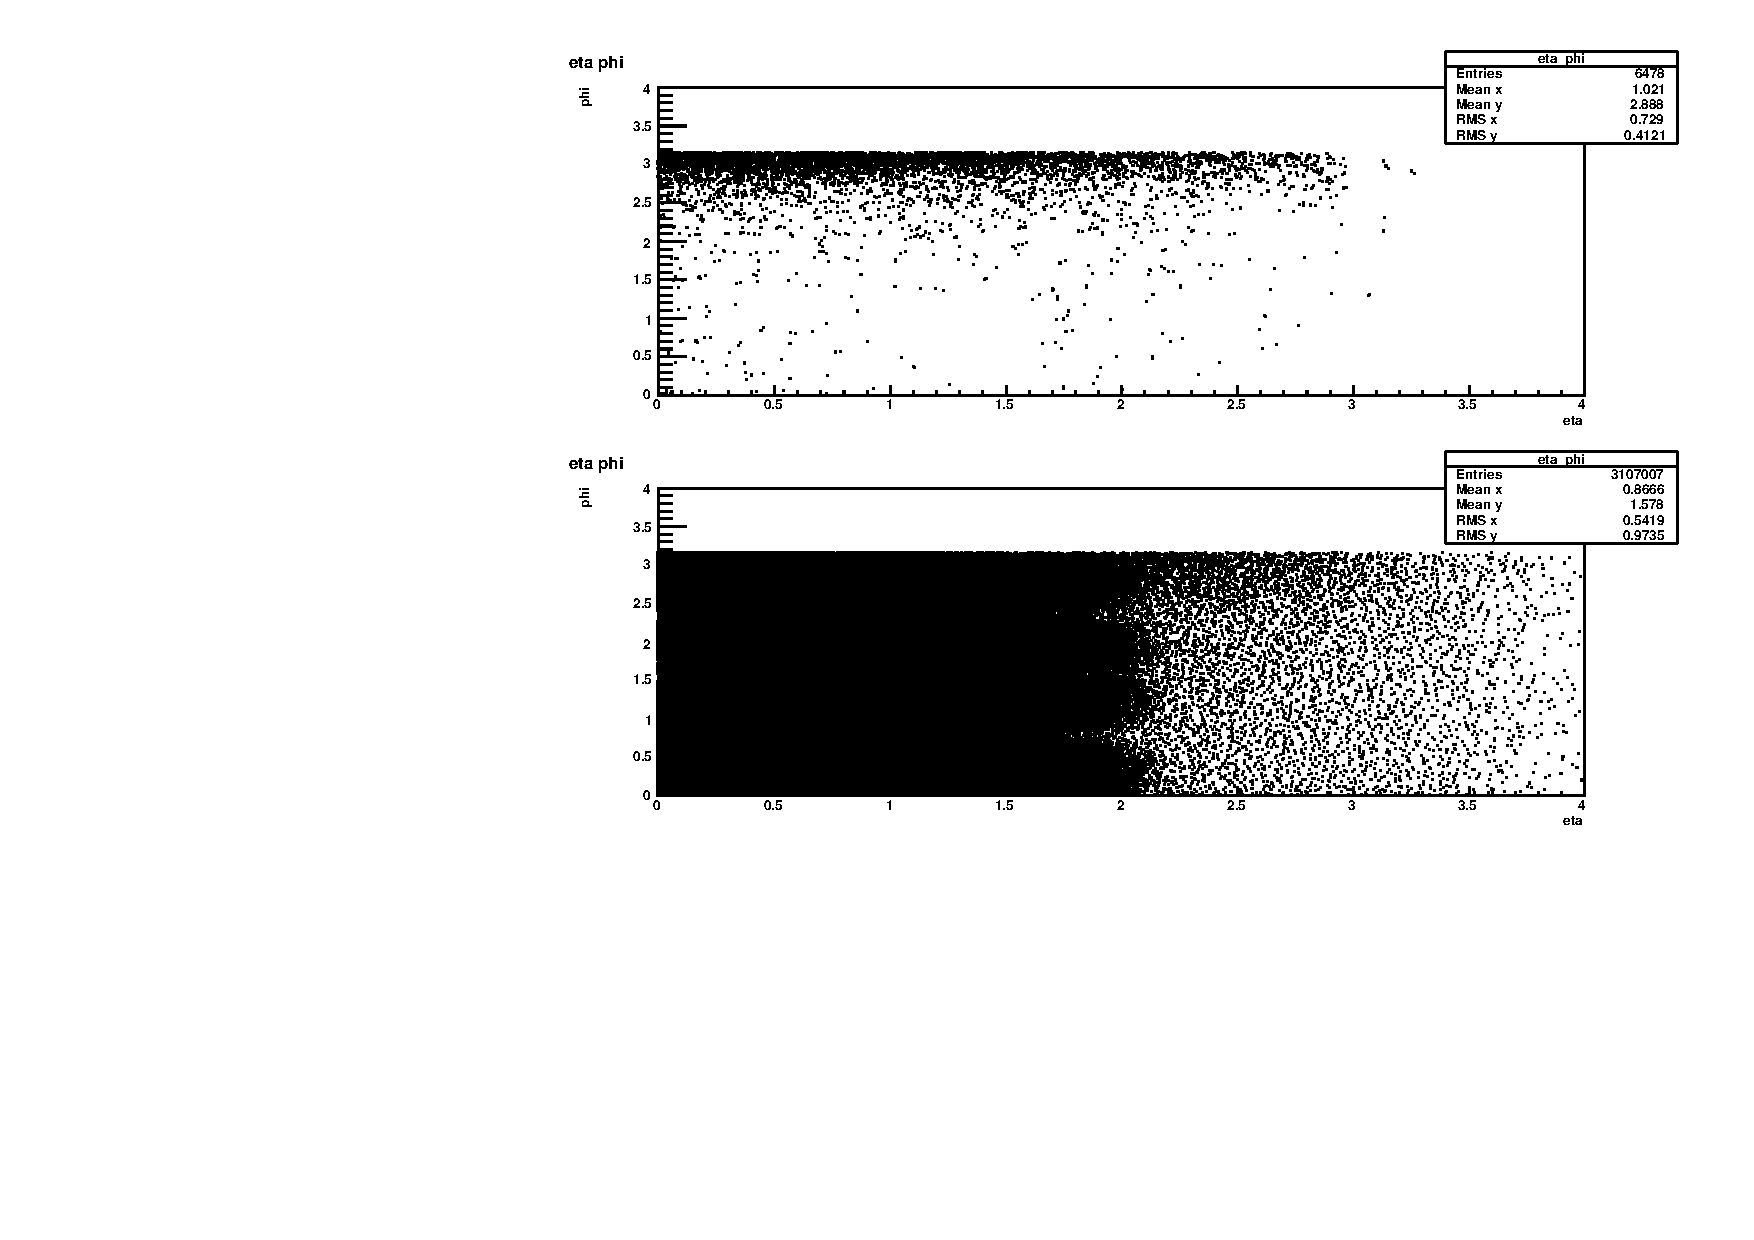
\includegraphics[width=0.9\textwidth]{fig/data_cut_etaphi.pdf}
        }
    \end{center}
    \caption{Two-dimensional histogram of the difference between pseudorapidity
    $\Delta\eta$ and difference between azimuthal angle $\Delta\phi$ of both muons
    for simulated (a) and real data (b). The upper plots are the accepted
    events, the lower plots are the rejected events. With the cuts detailed
    above, there is a clear preference of $\Delta\phi=\pi$ in both simulation
    and real data. Also, lower pseudorapidity difference $\Delta\eta$ is more
    common. For the uncut case, both simulation and real data shows additional
    structure at non-$2\pi$ azimuthal difference. Note that no angular cuts
    have been performed in either case.}
   \label{fig:angle}
\end{figure}

\subsection{Zmass}
The invariant $Z$ mass can be calculated directly with ROOT with the
TLorentz-vector class. In theory, the muon mass is not needed for a
reconstruction of the $Z$ events, as $E\approx p$ holds for the
ultrarelativistic case, which is fullfilled for the muons in question. Finally, with the cuts performed, the $Z$ mass is plotted in
\cref{fig:zmass1,fig:zmass2} for both $Z$ monte-carlo and real data.
One now clearly observes the expected mass peak also in the real data. The
rejected events mostly consist of low-$Z$-mass events and cut out very little
from the actual mass peak, which is especially apparent in the simulated data.
Again, a fit is performed for the Breit-Wigner curve \cref{eq:breit}. The
results are summarized in \cref{tab:fits}.

\begin{table}
    \centering
    \begin{tabular}{|c|c|c|}\hline
        Data set&$m_Z$\;[GeV]&$\Gamma_Z$\;[GeV]\\\hline
        $Z$ monte-carlo uncut&$90.69\pm0.06$&$7.612\pm0.071$\\\hline
        $Z$ monte-carlo cut&$91.64\pm0.03$&$4.448\pm0.088$\\\hline
        real data cut&$90.19\pm0.15$&$11.85\pm0.20$\\\hline
        \hline
        Theoretical result
        \cite{pdataz}&$91.1876\pm0.0021$&$2.4952\pm0.0023$\\\hline
    \end{tabular}
    \caption{Summary of reconstructed $Z$ mass $m_Z$ and decay width $\Gamma_Z$
    for both cut and uncut simulated data ,as well as real data obtained from
    the Breit-Wigner fit.}
    \label{tab:fits}
\end{table}


\begin{figure}
     \begin{center}
         \subfigure[]{
       \label{fig:zmass1}
            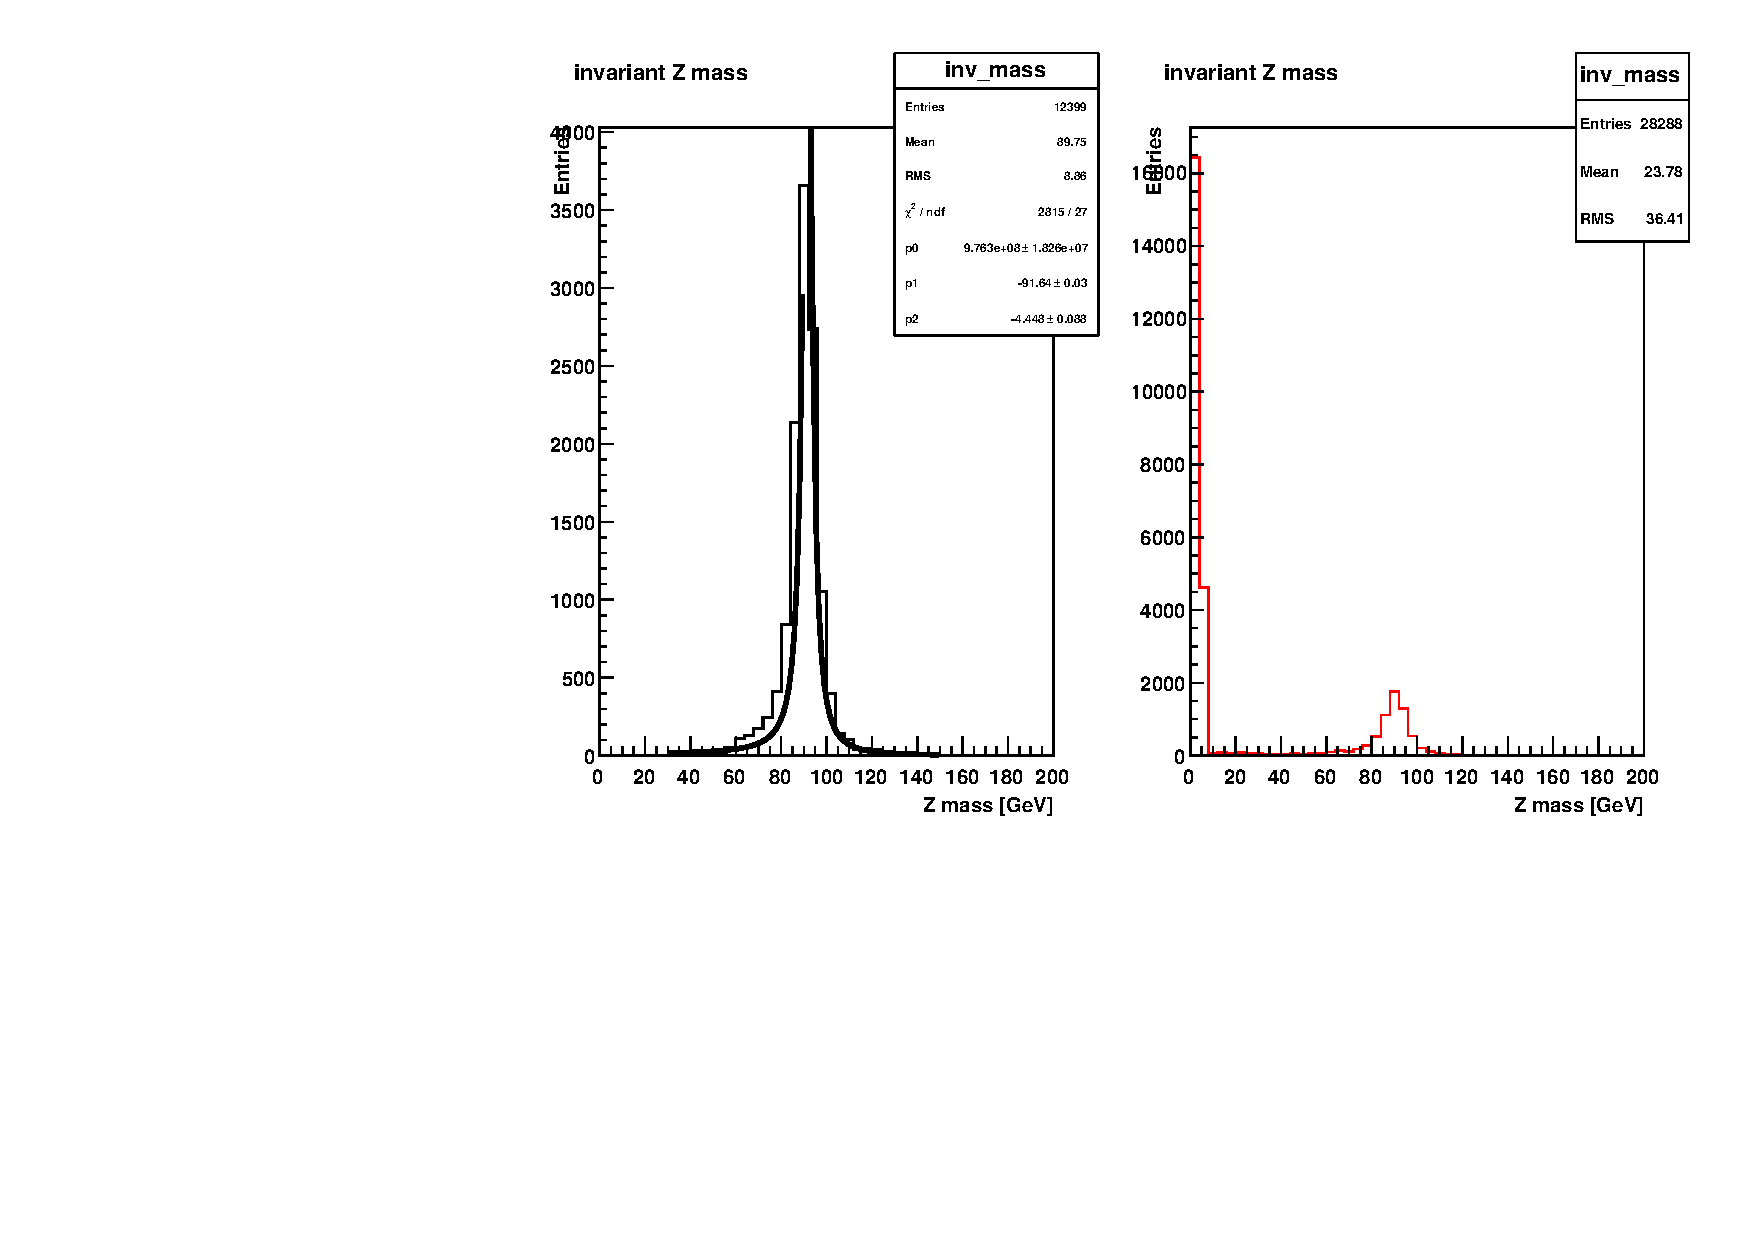
\includegraphics[width=0.9\textwidth]{fig/zmc_cut_zmass.pdf}
        }\\ %  ------- End of the first row ----------------------%
        \subfigure[]{
       \label{fig:zmass2}
            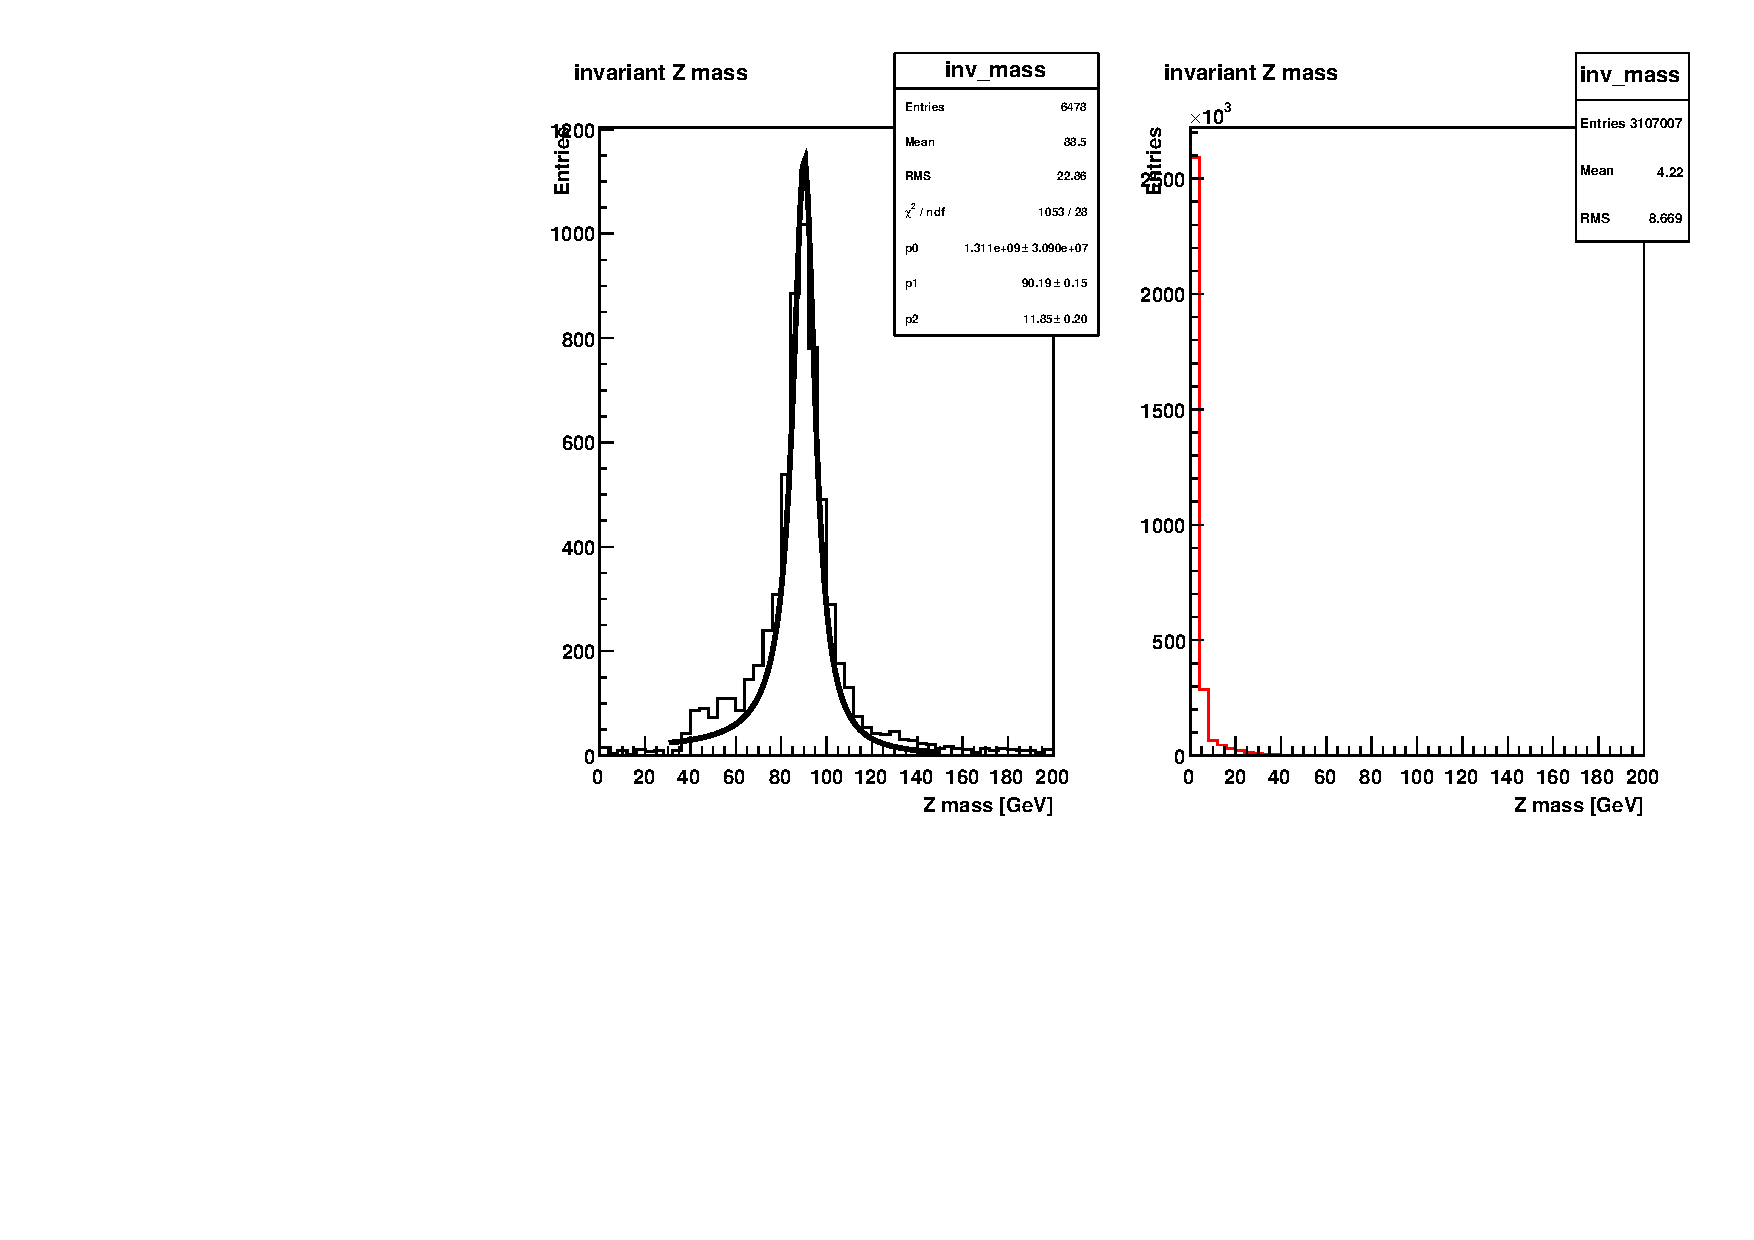
\includegraphics[width=0.9\textwidth]{fig/data_cut_zmass.pdf}
        }
    \end{center}
    \caption{Reconstructed $Z$ mass for the simulated (a) and real data (b). On
    the left in black, the accepted events are plotted, on the right the
    rejected ones. Apart from a small trail on the higher mass spectrum, both
    peaks look qualitatively the same. The cuts mostly got rid of the low $Z$-mass
    events, as can be seen by comparison of simulation and data. A
    $\chi^2$ fit for the Breit-Wigner curver is performed on the accepted
    events.}
\end{figure}


\subsection{Reconstructing and selecting $W$ events}
As outlined in \cref{sec:theory}, the invariant $W$ mass cannot be directly
reconstructed. This is due to the neutrino in the decay products, which is not
directly detectable. More specifically, the longitudinal momentum component of the $W$ is
outside of reach because of the composite structure of the colliding protons.
As a result, the total centre of mass energy is unknown on an event by event
basis. As the missing neutrino momentum can only be infered from the missing energy,
this means that the z-component of the energy is not detectable.
It is therefore the goal to define selections that reconstruct the transverse
mass \cref{eq:mt}. The uncut transverse mass of the $W$ monte-carlo simulation
is shown in \cref{fig:wuncut1}. As expected, it does not peak at the $W$ mass,
however the location of the dropoff fits the theoretical $W$ mass result of
$m_W=80.385\pm0.015$\;GeV \cite{pdataz}. The uncut real data plot
\cref{fig:wuncut2} does not have this feature: the background consisting mostly
of cosmics dominates in low transverse mass regions. In addition to the
object level cuts from \cref{tab:objectcuts}, different event level cuts are
performed:
\begin{itemize}
    \item $20\;\text{GeV}<$ MET $<60$\;GeV
    \item only one muon passes the trigger (since one muon and one neutrino is
        expected)
\end{itemize}
These two additional conditions are enough for a satisfactory reconstruction.
Cosmics are automatically filtered out, since they almost always correspond to
two muons detected at different times but only one muon is required with the
selections. The conditon for the missing transverse energy was mostly found by
trial and error and by comparing different paramenters of the simulated and the
real data. The resulting MET cuts are shown in \cref{fig:met1,fig:met2}. With
the cuts in place, both accepted distributions look similar.
Finally, the reconstructed transverse mass of the $W$ boson can be calculated
from \cref{eq:met}. It has to be kept in mind, that the muon is a minimal
ionising particle and therefore does not deposit its energy into the
calorimeter. Thus, when calculating the total missing transverse energy, the muon
momentum has to be added which in the relativistic case is
$E_T{_{\mu}}=p_{T_\mu}$. 

\begin{figure}
    \subfigure[]{
        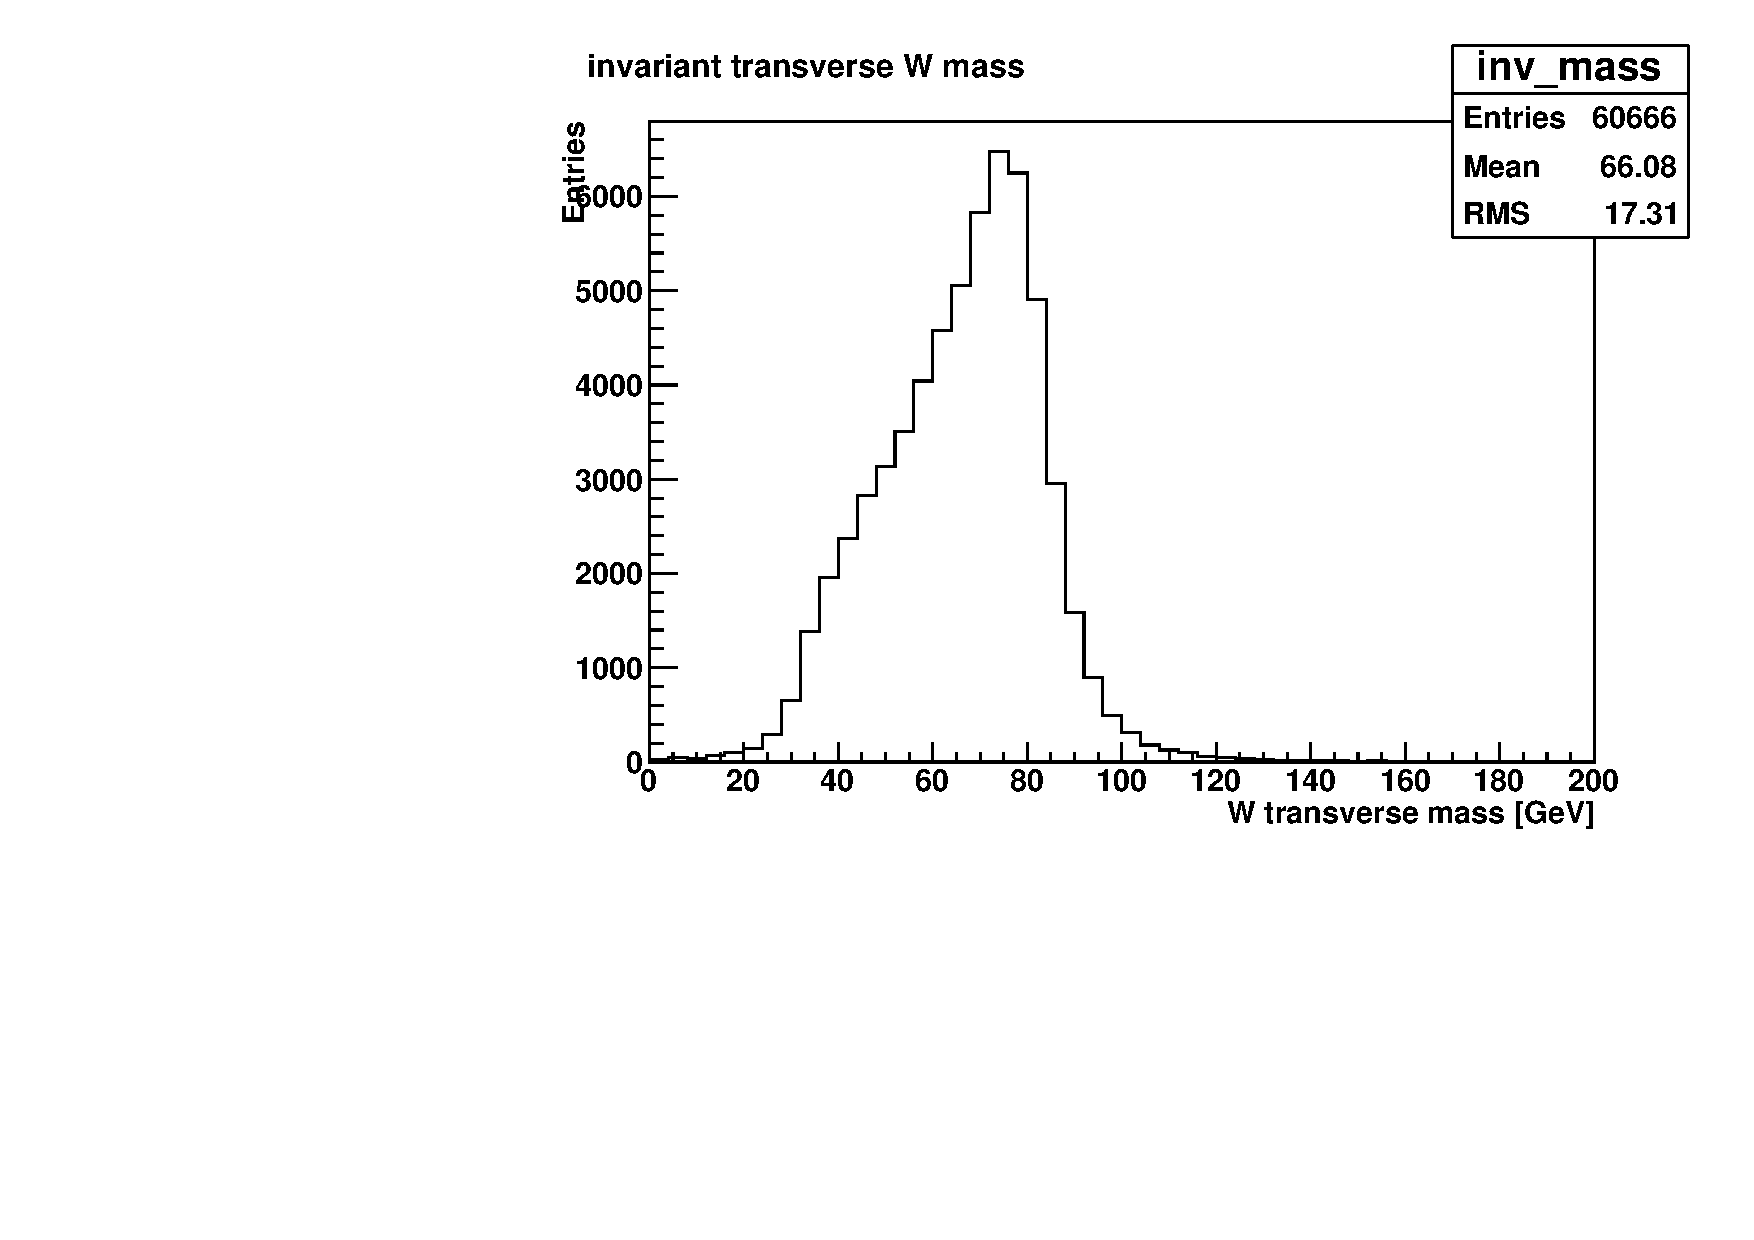
\includegraphics[width=0.45\textwidth]{fig/wmc_uncut_wmass.pdf}
        \label{fig:wuncut1}
    }
    \subfigure[]{
        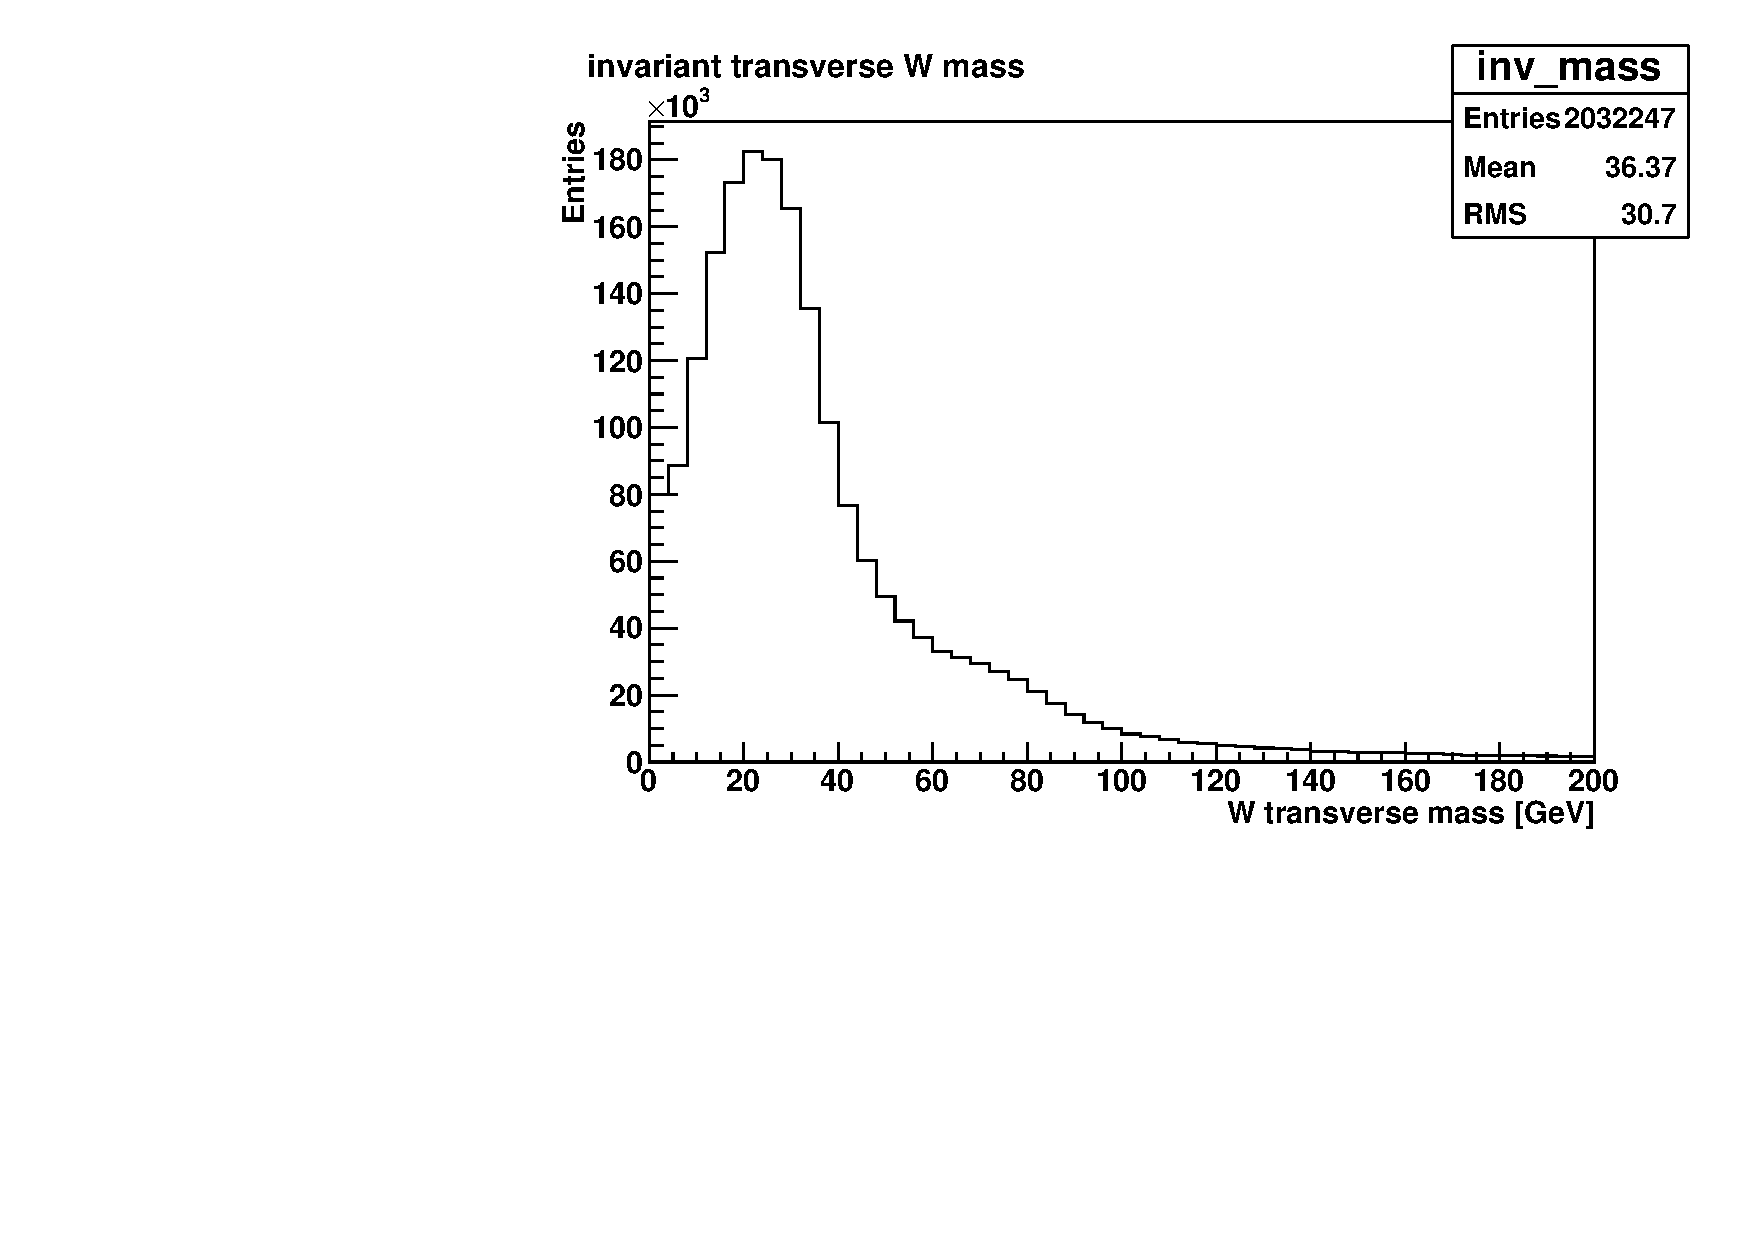
\includegraphics[width=0.45\textwidth]{fig/Wdata_uncut_wmass.pdf}
        \label{fig:wuncut2}
    }
    \caption{(a): Uncut transverse mass distribution of the $W$ monte-carlo
    simulation. The dropoff occurs at around 80\;GeV, which is consistent with
    the literature value. (b): Uncut transverse mass distribution of the real
    data. The data is dominated by low-transverse mass events.}
\end{figure}

\begin{figure}
    \subfigure[]{
        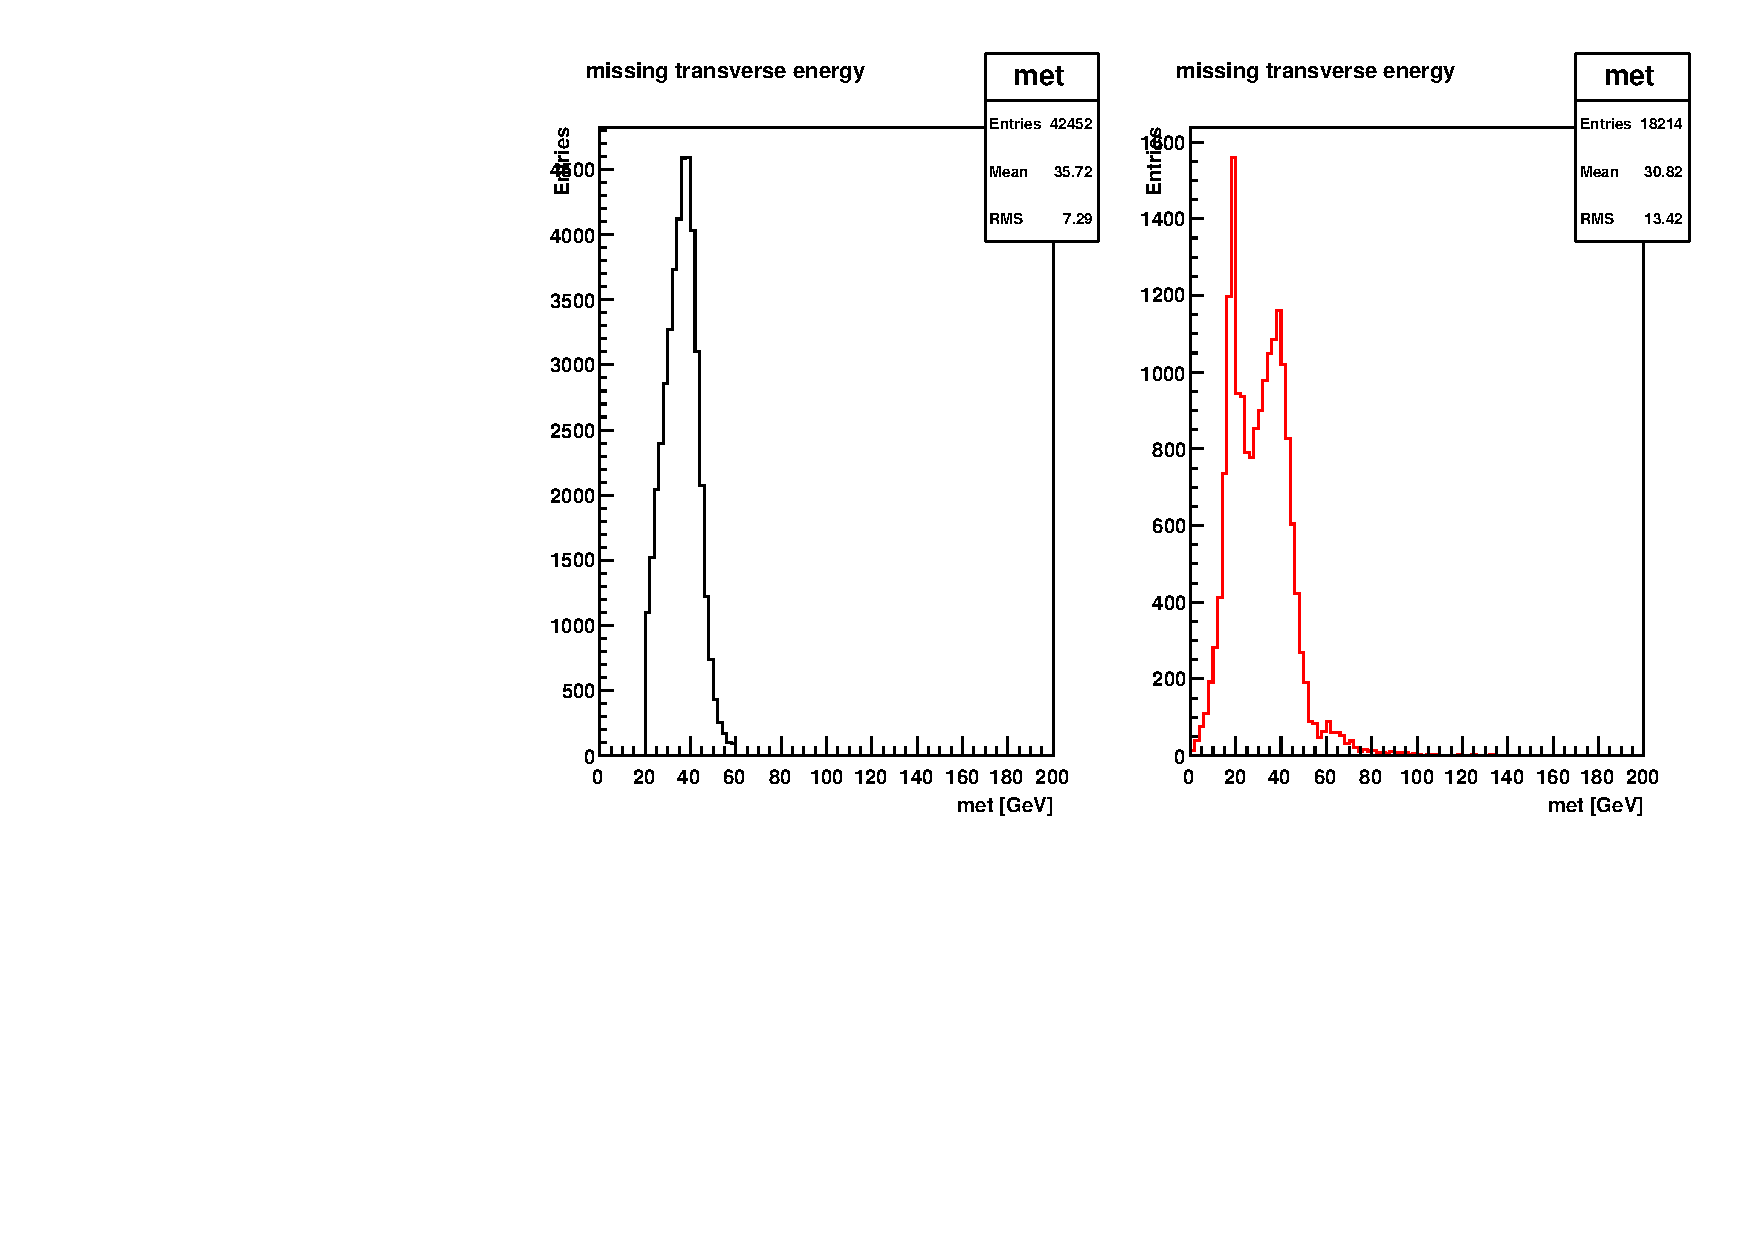
\includegraphics[width=0.5\textwidth]{fig/wmc_cut_met.pdf}
        \label{fig:met1}
    }
    \subfigure[]{
        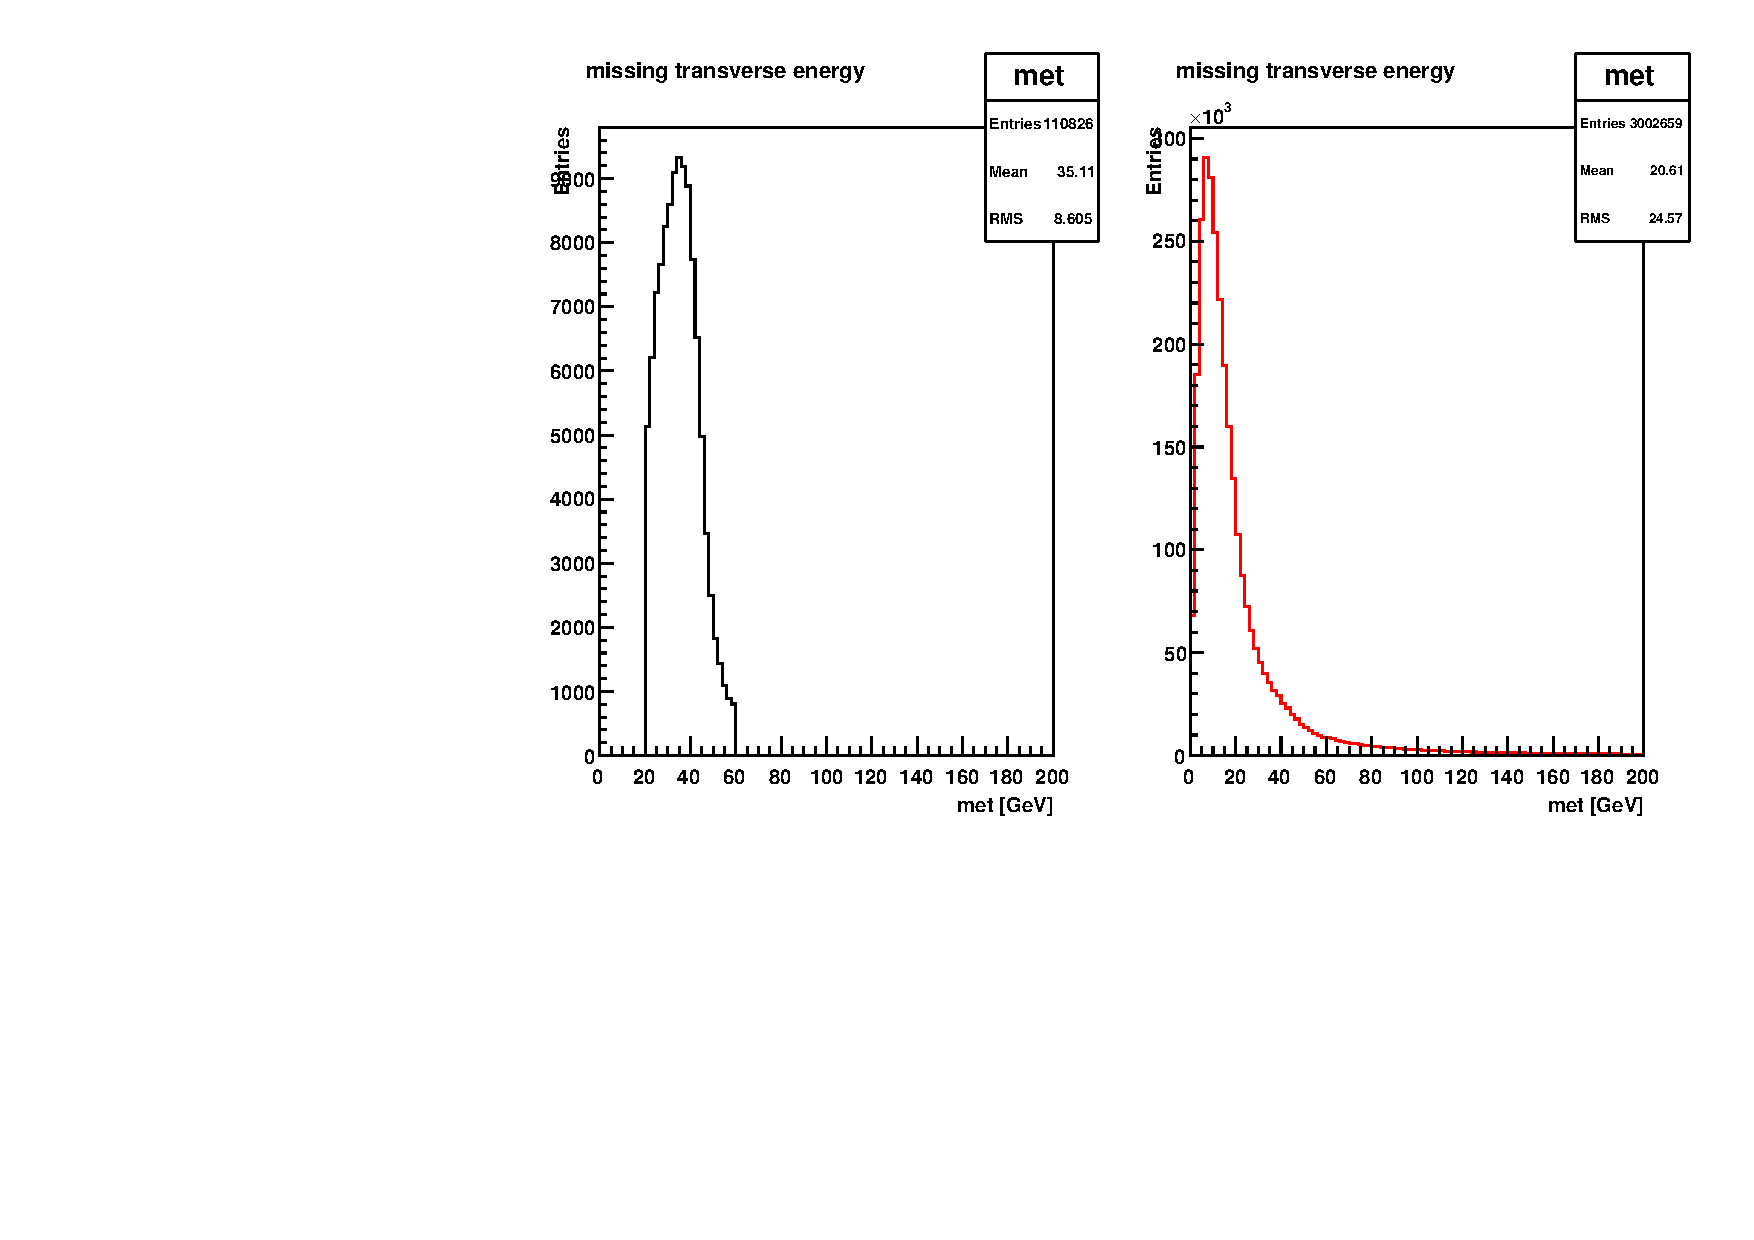
\includegraphics[width=0.5\textwidth]{fig/Wdata_cut_met.pdf}
        \label{fig:met2}
    }
    \caption{Missing transverse energy distribution for both simulation (a) and
    real data (b). Shown in black are the accepted events and in red are the rejected
    ones. With the cuts performed both accepted distributions look close to
    each other.}
\end{figure}



The resulting transverse energy is plotted in \cref{fig:metcut2}.
With cuts in place, the experimental data now also shows the expected dropoff
at around $80$\;GeV. Only around one percent of experimental events passed the
selection criteria. Mostly low $m_T$ background was rejected. Still, also about
one third of monte-carlo events were rejected, which might indicate an
overselection.

\begin{figure}
     \begin{center}
         \subfigure[]{
       \label{fig:metcut1}
            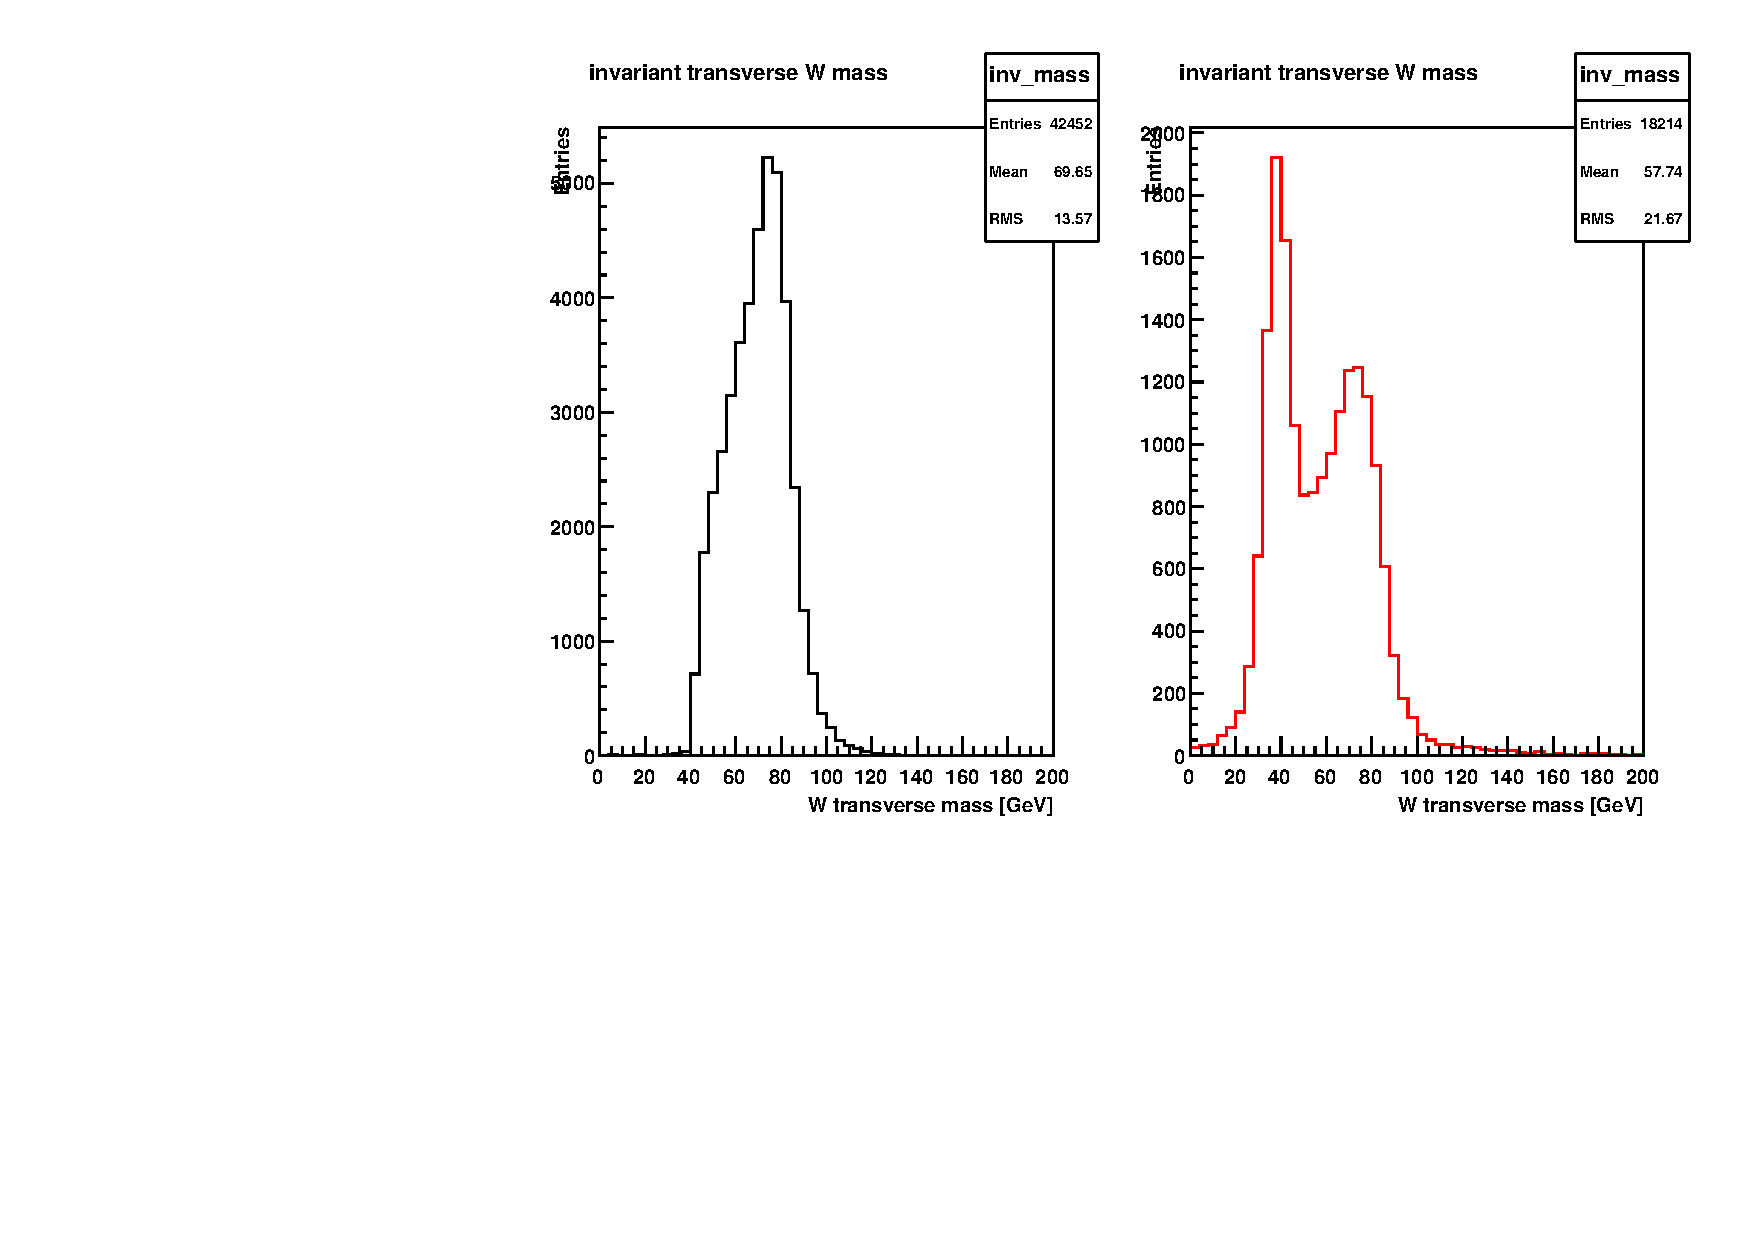
\includegraphics[width=0.9\textwidth]{fig/wmc_cut_wmass.pdf}
        }\\ %  ------- End of the first row ----------------------%
        \subfigure[]{
       \label{fig:metcut2}
            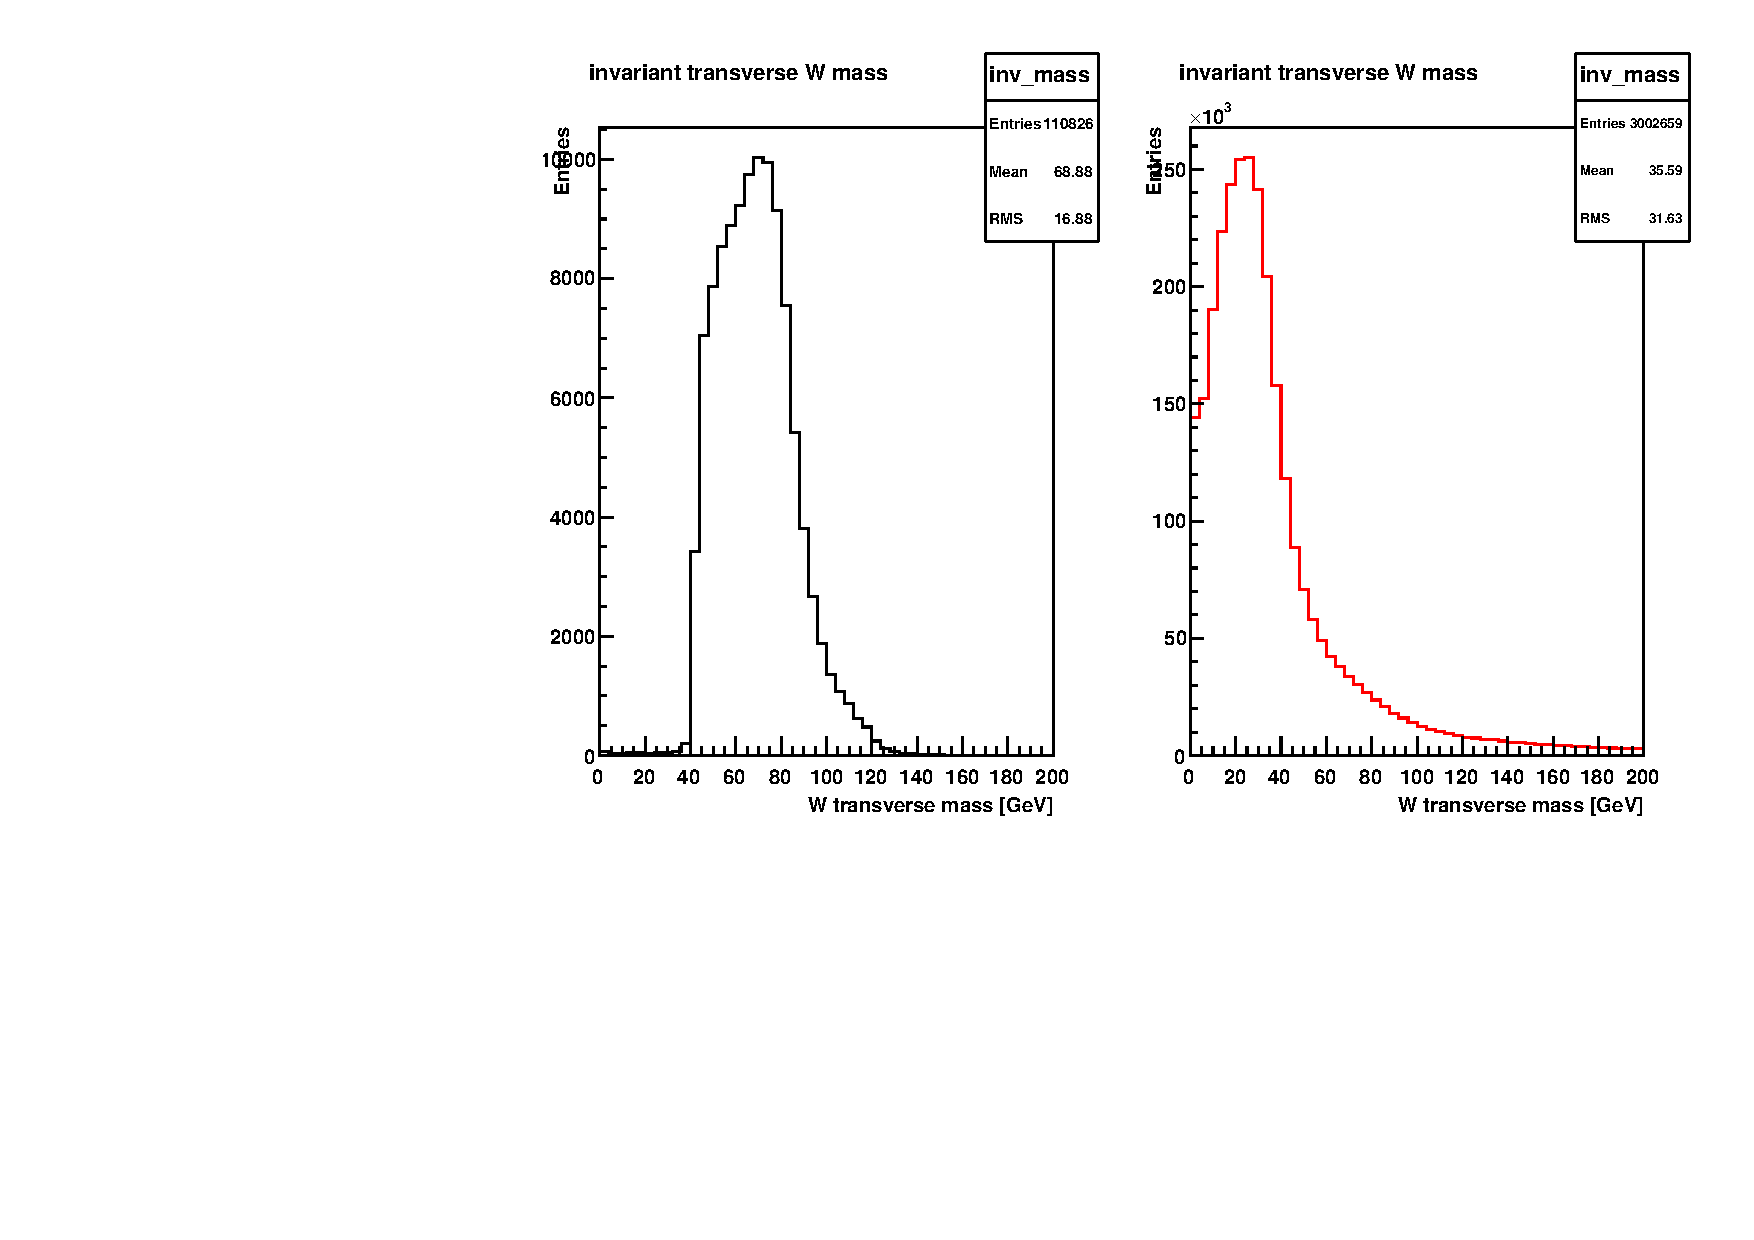
\includegraphics[width=0.9\textwidth]{fig/Wdata_cut_wmass.pdf}
        }
    \end{center}
    \caption{Reconstructed transverse $W$ mass for the simulated data with cuts
    (a) and for the cut real data (b). In black: selected events. In red:
    rejected events. The selection mostly rejected low $m_T$ background. The expected dropoff at around $80$\;GeV is now visible
    for the experimental data. However, also about one third of monte-carlo
    events were rejected by our selection.}
\end{figure}


\subsection{Determination of efficiencies}
In order to calculate the branching ration in \cref{ss:br}, one first has to
calculate both the trigger- and the reconstruction efficiencies. The trigger
efficiency is needed, since not every muon event will trigger within the
detector. The ones that are missed have to be accounted for. The trigger
efficiency is calculated by the independent trigger method: First, the number
of events $N_\text{indep}$ are counted that pass the independant trigger
$TRIG_\text{Independant}$, as well as all object level cuts.
The independent trigger is only determined by certain calorimeter conditions and therefore
unhinged from the muon detection. Next, all events $N_\text{trig}$ that
additionally pass the MUW\_W\_L2M3\_TRK10 trigger used in the analysis prior is
calculated.
The ratio
\begin{align}
    \label{eq:trigeff}
    \epsilon_\text{trig}=\frac{N_\text{trig}}{N_\text{indep}}
\end{align}
is called the trigger efficiency.
One obtains
\begin{align}
    \label{eq:trigeffvalue}
    \epsilon_\text{trig}=0.623.
\end{align}
The question now, is how to gauge the error for this efficiency. One way is to
calculate the standard deviation of a binonial distribution
\begin{align}
    \label{eq:binomial}
    P(k|n,\epsilon_{trig})=\frac{n!}{k!(n-k)!}\epsilon^k(1-\epsilon)^{n-k}.
\end{align}
This seems appropriate, since the probability that the special trigger is
passed for a single event out of the number of all independent events $n$ is
independent from all other events and also identically distributed. Therefore,
we have a sum of independent, identically distributed random variables, which
gives the probability that $k$ out of $n$ independent events pass the
trigger. The variance for the number of passed events $k$ is now
$V(k)=n\epsilon(1-\epsilon)$ \cite{efferror}, from which follows via error
propagation
\begin{align}
    \label{eq:kstd}
    V(\epsilon)=V(k/n)=\frac{V(k)}{n^2}=\frac{\epsilon(1-\epsilon)}{n}.
\end{align}
The potential problem with this treatment is that the trigger efficiency
$\epsilon$ is what is calculated and not given. Therefore, the error depends on
the measurement of $\epsilon$. A more correct approach would be to use
bayes-theorem and calculate the probability that $\epsilon$ is the real
efficiency, based on the measurements of $k$ and $n$. More detail can be found
in \cite{efferror}. Here, we assume that the binomial approach works,
especially since the biggest uncertainty comes from the reconstruction
efficiencies. We thus have for the uncertainty
\begin{align}
    \label{eq:uncerteff}
    \sigma_{\epsilon_\text{trig}}=\sqrt{V(\epsilon_\text{trig})}=\sqrt{\frac{\epsilon_\text{trig}(1-\epsilon_\text{trig})}{n}}.
\end{align}
Unfortunately it was forgotten to calculate the number of events that pass the
independent trigger $n$. In the uncut case we had around 3 million events. Even
with the very strict guess that only $n=50000$ events were to pass the
independent trigger, this would mean an uncertainty of
$\sigma_{\epsilon_\text{trig}}=0.002$, which is a reasonable value considering
that the errors for the reconstruction uncertainties can only be guessed as
well. For the $Z$ boson, the trigger efficiency has to be slightly modified,
since there are two seperate muons that can be detected:
\begin{align}
    \label{eq:trigeffZ}
    \epsilon_\text{trig,Z}=\epsilon_\text{trig}^2+\epsilon_\text{trig}(1-\epsilon_\text{trig})+(1-\epsilon_\text{trig})\epsilon_\text{trig}=-\epsilon_\text{trig}^2+2\epsilon_\text{trig},
\end{align}
which is the sum of the probabilities that both muons trigger and the
probability that exactly one muon triggers.

Next, the reconstruction efficiencies are determined, which for both bosens are
defined by
\begin{align}
    \label{eq:receff}
    \epsilon_\text{rec}=\frac{\text{\# of reconstructed events in
    monte-carlo}}{\text{\# total events in monte-carlo}}.
\end{align}
The results are
\begin{align}
    \label{eq:receffres}
    \epsilon_\text{rec,W}=\frac{42452}{60666}=0.700,\qquad
    \epsilon_\text{rec,Z}=\frac{12399}{40687}=0.305.
\end{align}
Additionaly, the misidentification rate
\begin{align}
    \label{eq:miss}
\epsilon_\text{miss}=\frac{\text{\# reconstructed fake $W$
bosons}}{\text{\# total $Z$ bosons}}=\frac{14641}{40687}=0.360
\end{align}
 has to be taken into
acount. It is calculated by running the $W$ selection algorithm over the $Z$
monte-carlo data to find how many are misidentified.
It has to be assumed that this misidentification rate as calculated solely for
the simulated data reflects the real world misidentification of $W$ bosons.
This is a crude approximation. Idially one would like to directly calculate
this value from the experimental data. For this one would need to identify
events where a muon is detected but none is found, which is out of scope
of this report. For more details see the ``tag and probe method`` \cite{tagprobe}.

\subsection{Determination of the $BR(W\rightarrow\mu\nu)$}
The theoretical cross sections are given in \cite{fprakt}:
\begin{itemize}
    \item $\sigma(p\bar p\rightarrow W+X)=23.7\;$nb
    \item $\sigma(p\bar p\rightarrow Z+X)=7.18\;$nb
    \item $BR(Z\rightarrow\mu\mu)=3.366\pm0.007\%$.
\end{itemize}
The ratio of $W$ and $Z$ events is given by \cite{fprakt}
\begin{align}
    \label{eq:R}
    R=\frac{\sigma(p\bar p \rightarrow W+X)BR(W\rightarrow\mu\nu)}{\sigma(p\bar
    p \rightarrow Z+X)BR(Z\rightarrow\mu\mu)}=\frac{N_W}{N_Z},
\end{align}
where $N_{W/Z}$ is the total amount of real $W/Z$ events (not just those that
passed the trigger). The integrated luminosity is not needed as it cancels out. The number of reconstructed events can be written in terms
of the true number contained in the data:
\begin{align}
    \label{eq:waddap}
    N_{\text{rec},W}&=(N_W \epsilon_\text{rec,W}+N_Z\epsilon_\text{miss})\epsilon_{\text{trig},W},\\
    N_{\text{rec},Z}&=(N_W \epsilon_\text{rec,Z})\epsilon_{\text{trig},Z}
\end{align}
Rearranging the terms from \cref{eq:R,eq:waddap} one finally obtains
\begin{align}
    \label{eq:BRRR}
    BR(W\rightarrow\mu\nu)=(\frac{N_{\text{rec},W}\epsilon_{\text{rec},Z}\epsilon_{\text{trig},Z}}{N_{\text{rec},W}\epsilon_{\text{rec},Z}\epsilon_{\text{trig},Z}}-\frac{\epsilon_{\text{miss}}}{\epsilon_{\text{rec},W}})\frac{\sigma(p\bar
    p\rightarrow Z+X)BR(W\rightarrow\mu\mu)}{\sigma(p\bar p\rightarrow
    W+X)}=9.95\%.
\end{align}


\label{ss:br}
\section{Discussion}
\label{sec:discussion}


First, it has to be pointed out that overall very few event level cuts have
been used. Almost all cuts have been object level $p_T$, $\chi^2$ and
$E_\text{halo}$ cuts, which are identical for both $Z$ and $W$ analysis.
The only event level cuts used were the charge of the muon(s) and their number.
It seems surprising that the $Z$ mass could still be reconstructed
successfully, as can be seen in \cref{tab:fits}. Neither of the values are
within their one sigma confidence intervals that the fit gave us, however both
the uncut monte-carlo, as well as the cut monte-carlo and the measured value
with the real data is very close to the literatue value with a maximal relative
difference of 1\% with the real data value. Both monte-carlo results have the
same relative difference of 0.5\% and are therefore slightly more accurate.
The theoretical decay width is almost one order of magnitude lower than the
measured value. This can be explained by the fact that the reconstructed, not
the actual $Z$ mass peak was measured. Spectral broadening inside of the
detector tends to widen the variance of the data.\\ The reconstructed $Z$-mass plot \cref{fig:zmass2} shows a qualitatively very
good  reconstruction of the peak. It can also be seen that the selection
conditions mostly eliminated low $m_T$ background. As our analysis suggests
this background consists mostly of cosmics: A muon going through both sides of
the detector gives effectively the muon's rest mass as invariant mass.
The fact that the selection conditions were enough probably rests on the charge
cuts that instantly filter out the cosmic events (that all have the same
charge) without needing to further analyse the angular distributions.
But there is also the risk of overcutting: On the one hand, around two thirds
of the monte-carlo data has been cut out by our selections. On the other hand,
most of the rejected data consists of the background as evident in
\cref{fig:zmass1}.\\
For the $W$ boson, only the MET cuts aswell as the forced number and charge of
muons have been utilised. Qualitatively the reconstructed $W$ transverse mass
distribution looks very promising. A detailed determination of the $W$ mass was
not done however, and might make the result less optimal. Hints for this are
seen in the $W$ monte-carlo plots \cref{fig:metcut1,fig:metcut2}: The selection
rejected around one third of the $W$ monte-carlo events. Therefore there has
probably been an overselection of events. A larger focus on event-based cuts
like angular distribution should be done before doing strict object-level cuts,
as we have done. Especially more 2d-histograms could have helped to find the
right selections.\\
Another improvement can be made for the trigger efficiency, for which it was
forgotten to calculate the number of events that pass the independent trigger.
It is questionable whether the crude approximation of $n=50\,000$ events is
reasonable, but it was used to create an approximate upper bound to the error,
since the error only shrinks with a larger $n$.\\
The reconstruction efficiencies \cref{eq:receffres} show, that $W$ events are
more effectively reconstructed than $Z$ events. However, also about one third
of all $Z$ bosons are misidentified as a $W$ boson. Still, these efficiencies
were calculated with the simulated data only. There is no guarantee that the
real data behaves in the same way to the cuts we have chosen.
Finally, the branching ratio of the $W$ boson that was measured here has a 7\%
relative difference to the literature value. While this has the right order of
magnitude, one cannot be confident with this value, because no real error
propagation could be calculated without the tag and probe method. 
Summing up, this lab has provided a very nice introduction into data analysis
with root, as well as standard practices commonly used in particle physics.
With more background knowledge one could have spent more time on finetuning the
selections which in turn could have provided a better end result. Still,
qualitatively one can be content with the result that was found in a few hours
of data analysis.
\bibliography{literatur}
\newpage
\begin{appendices}
\section{$Z$ boson additional plots}
\label{app:z}
\begin{sidewaysfigure}
%\begin{figure}[ht!]
     \begin{center}
         \subfigure[]{
            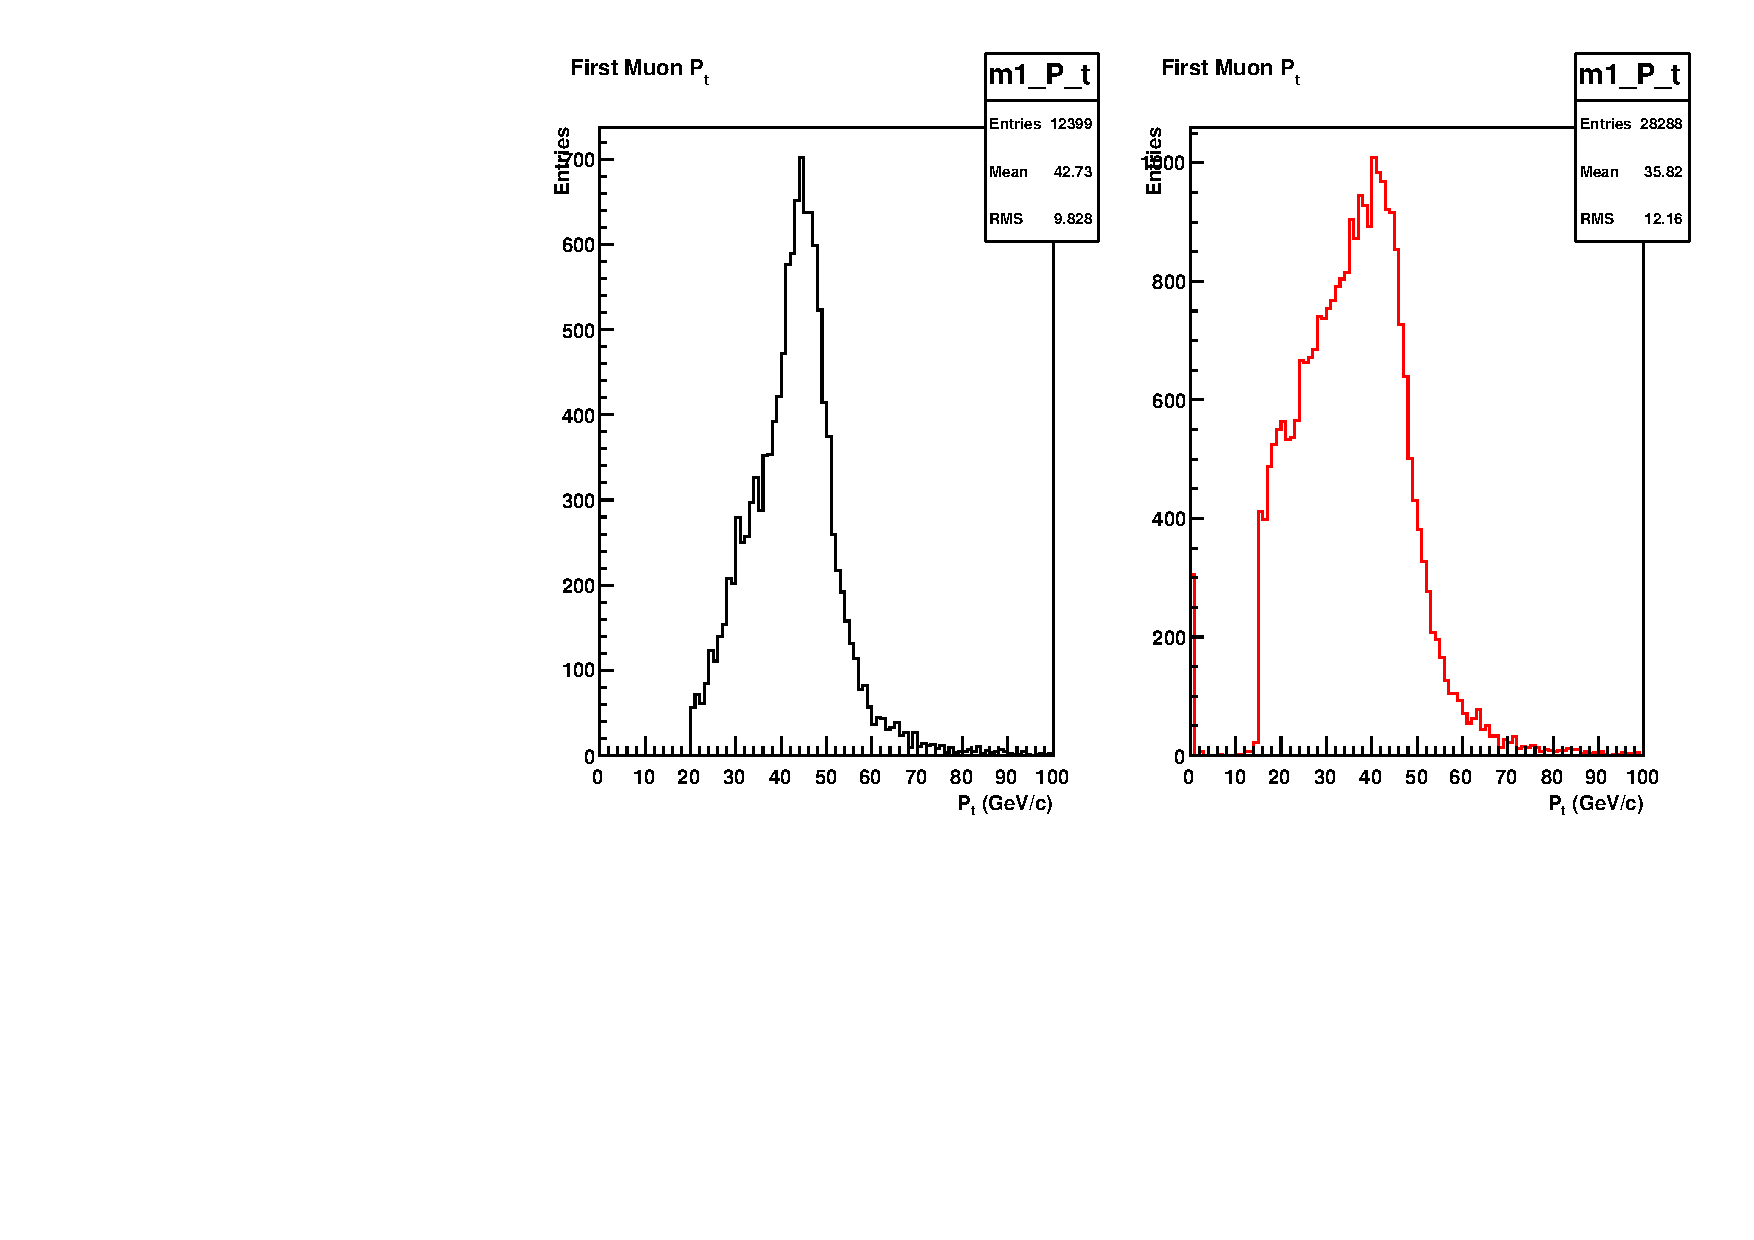
\includegraphics[width=0.45\textwidth]{fig/zmc_cut_muonpt_1.pdf}
        }
        \subfigure[]{
            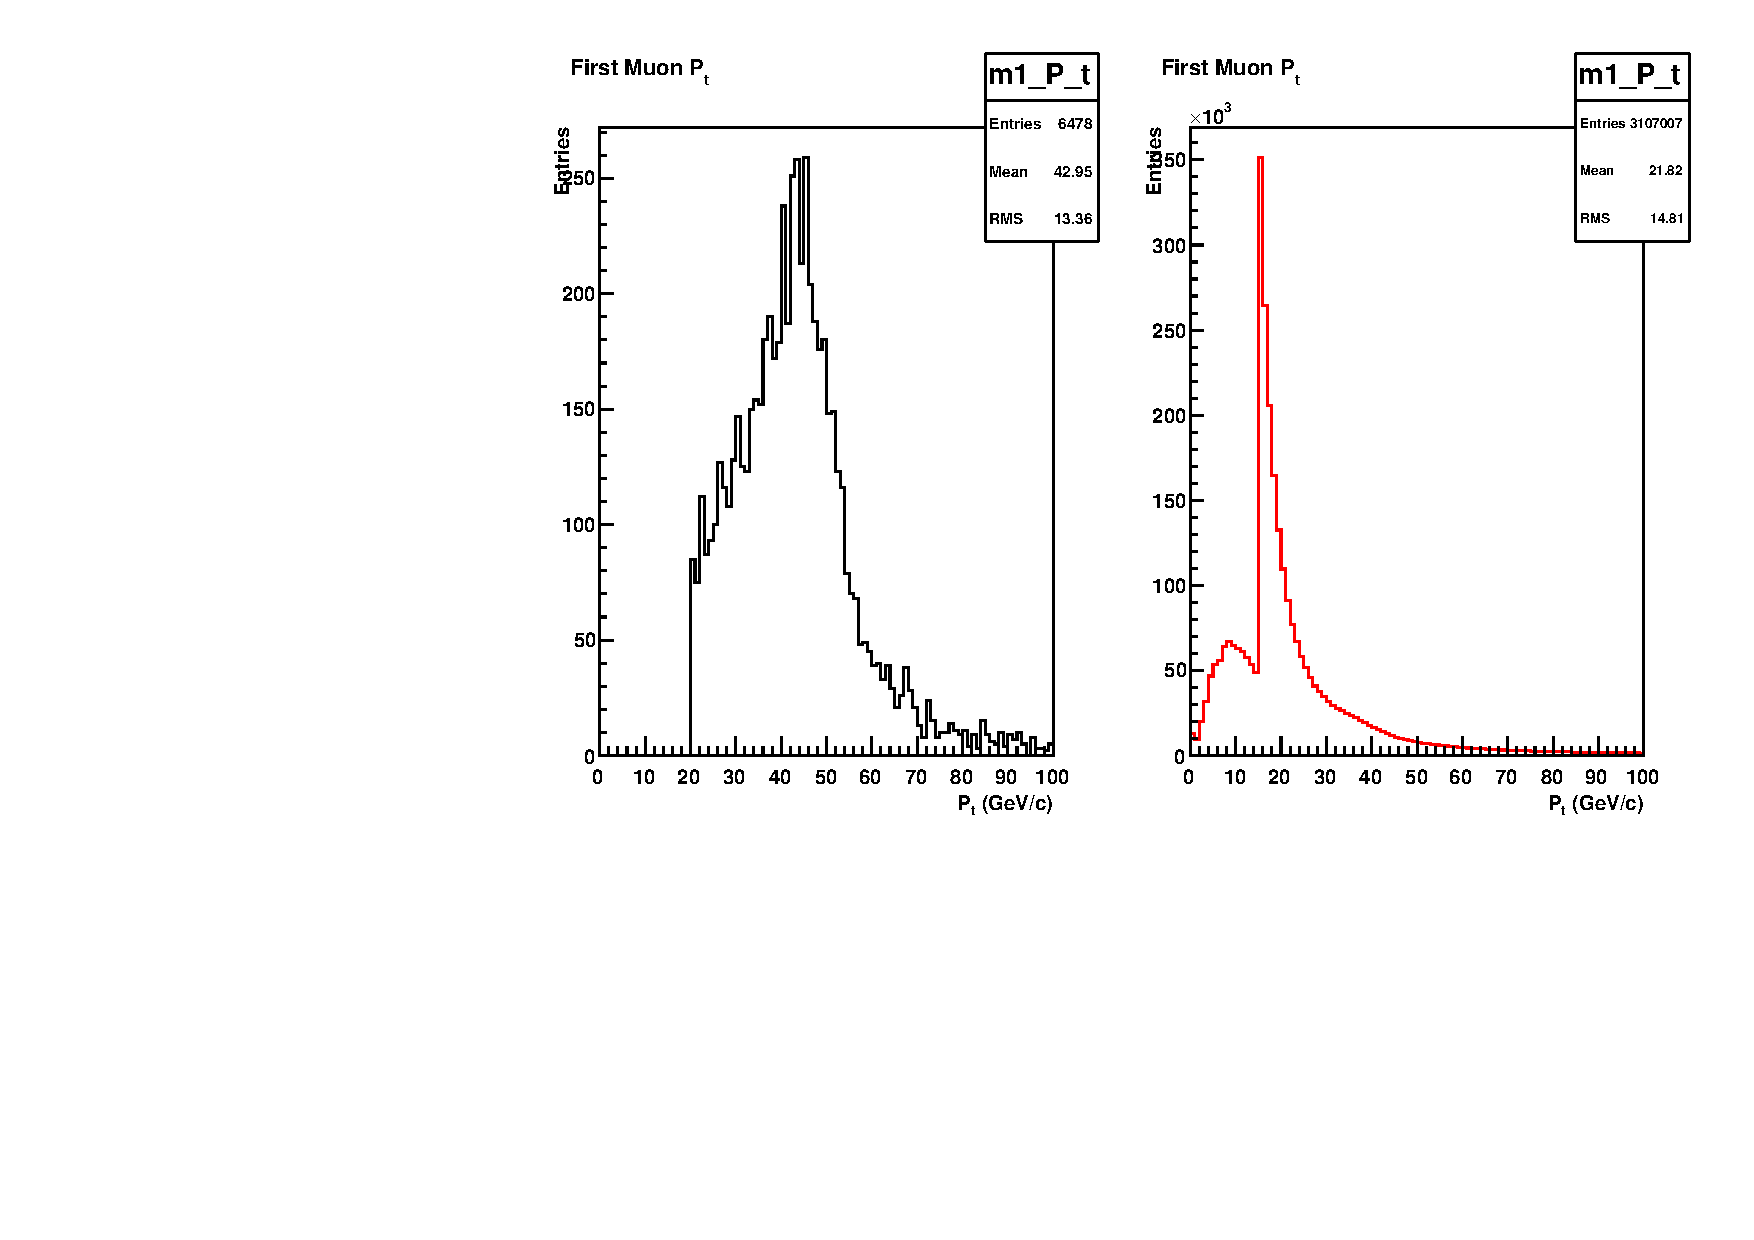
\includegraphics[width=0.45\textwidth]{fig/data_cut_muonpt_1.pdf}
        }\\ %  ------- End of the first row ----------------------%
        \subfigure[]{
            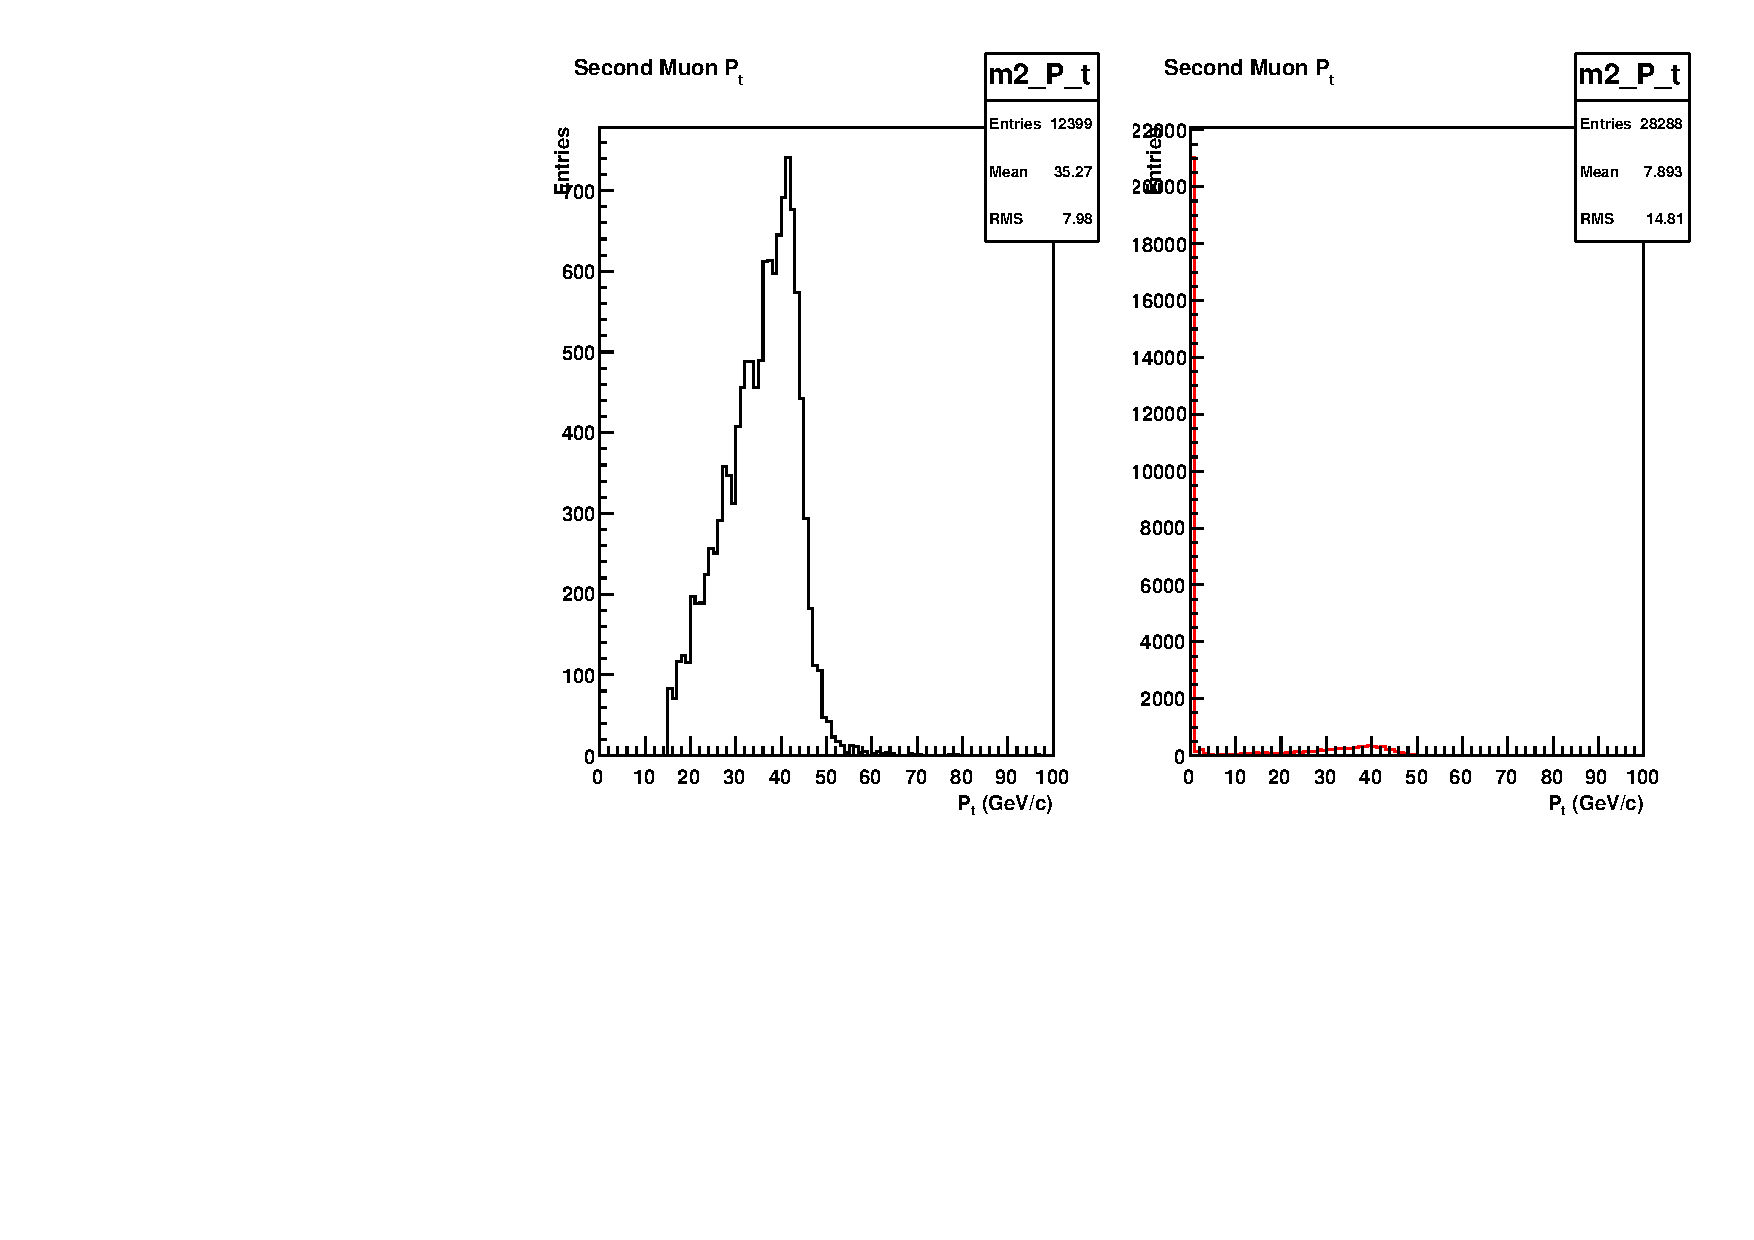
\includegraphics[width=0.45\textwidth]{fig/zmc_cut_muonpt_2.pdf}
        }
        \subfigure[]{
            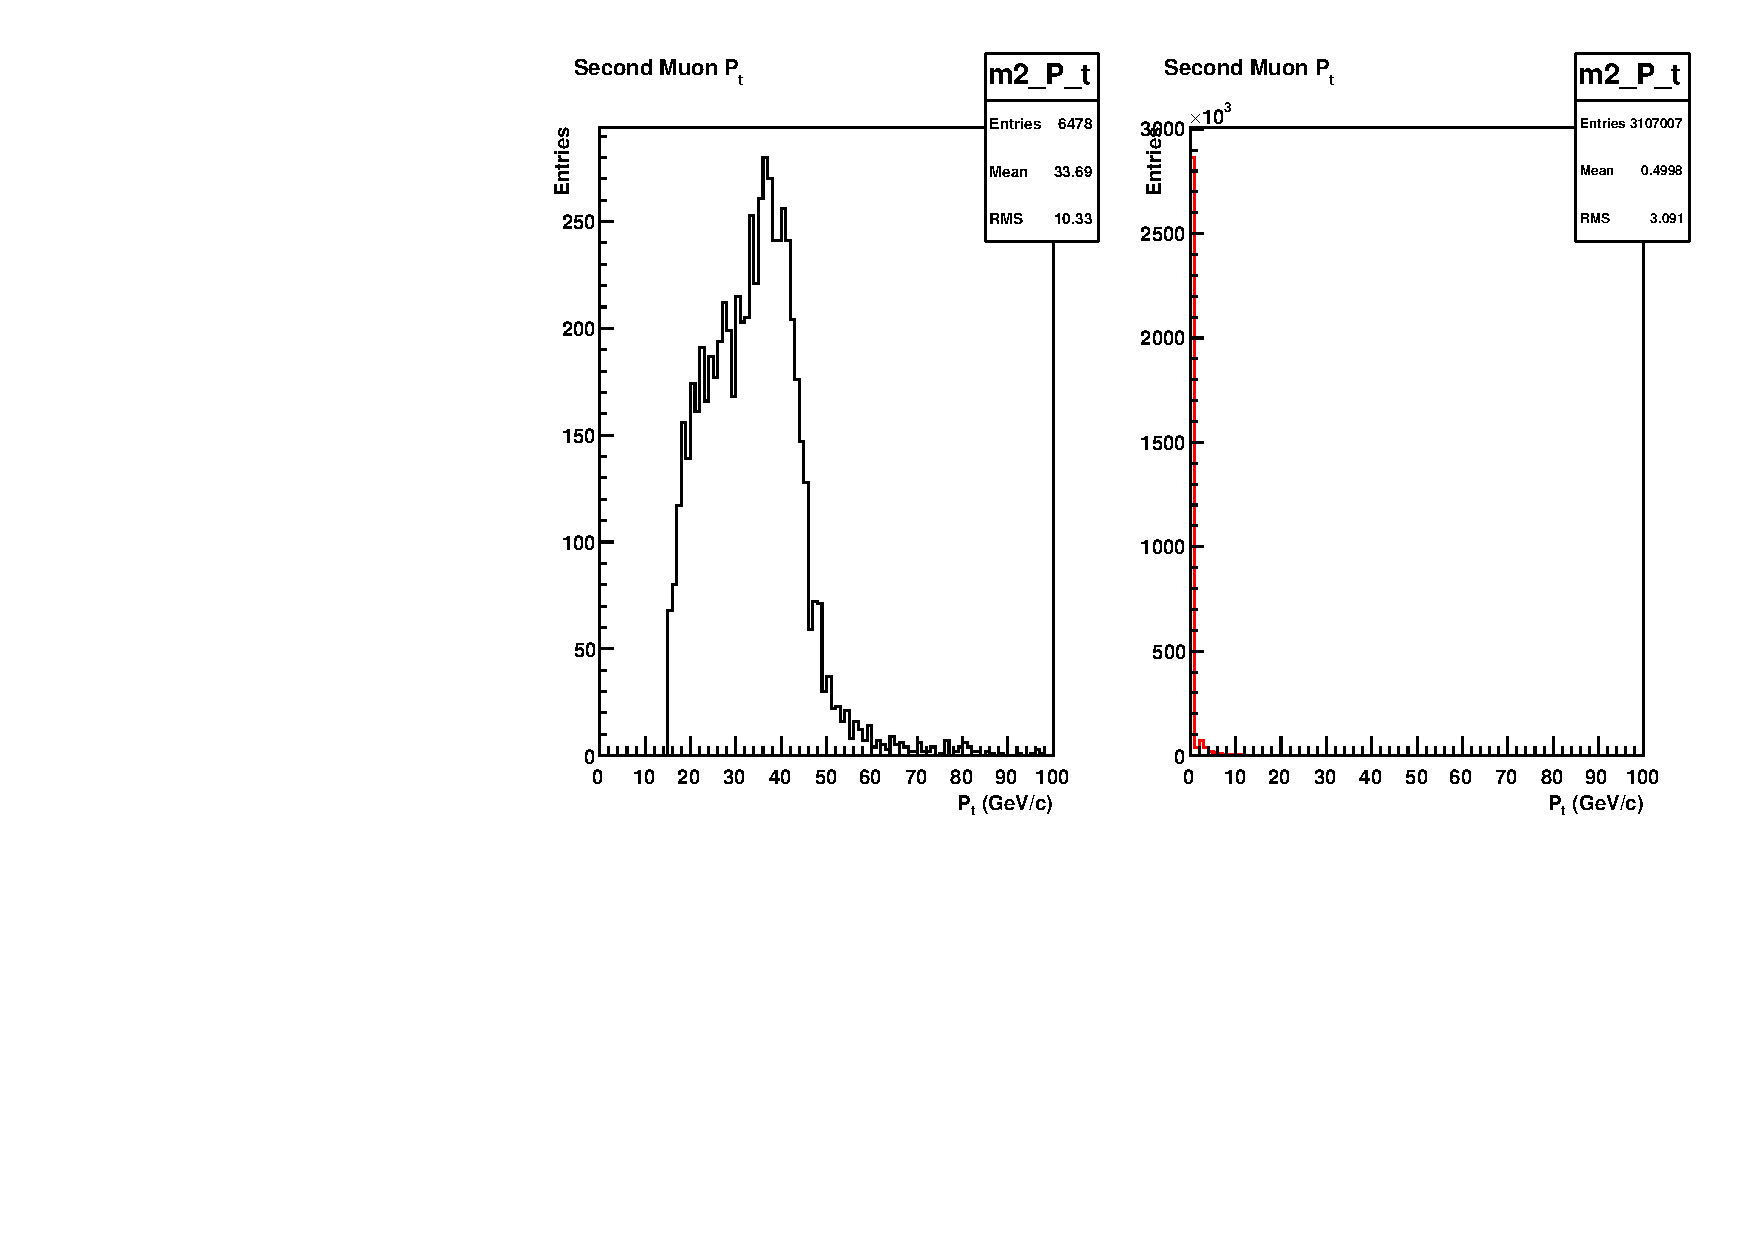
\includegraphics[width=0.45\textwidth]{fig/data_cut_muonpt_2.pdf}
        }
    \end{center}
    \caption{
        $p_{T}$ for accepted (black) and rejected (red) events
            for (a,c): the $Z$ monte-carlo data (b,d): the real data.}{
     }
   \label{fig:pt}
%\end{figure}\bibliography{literatur}
\end{sidewaysfigure}
\begin{sidewaysfigure}
%\begin{figure}[ht!]
     \begin{center}
         \subfigure[]{
            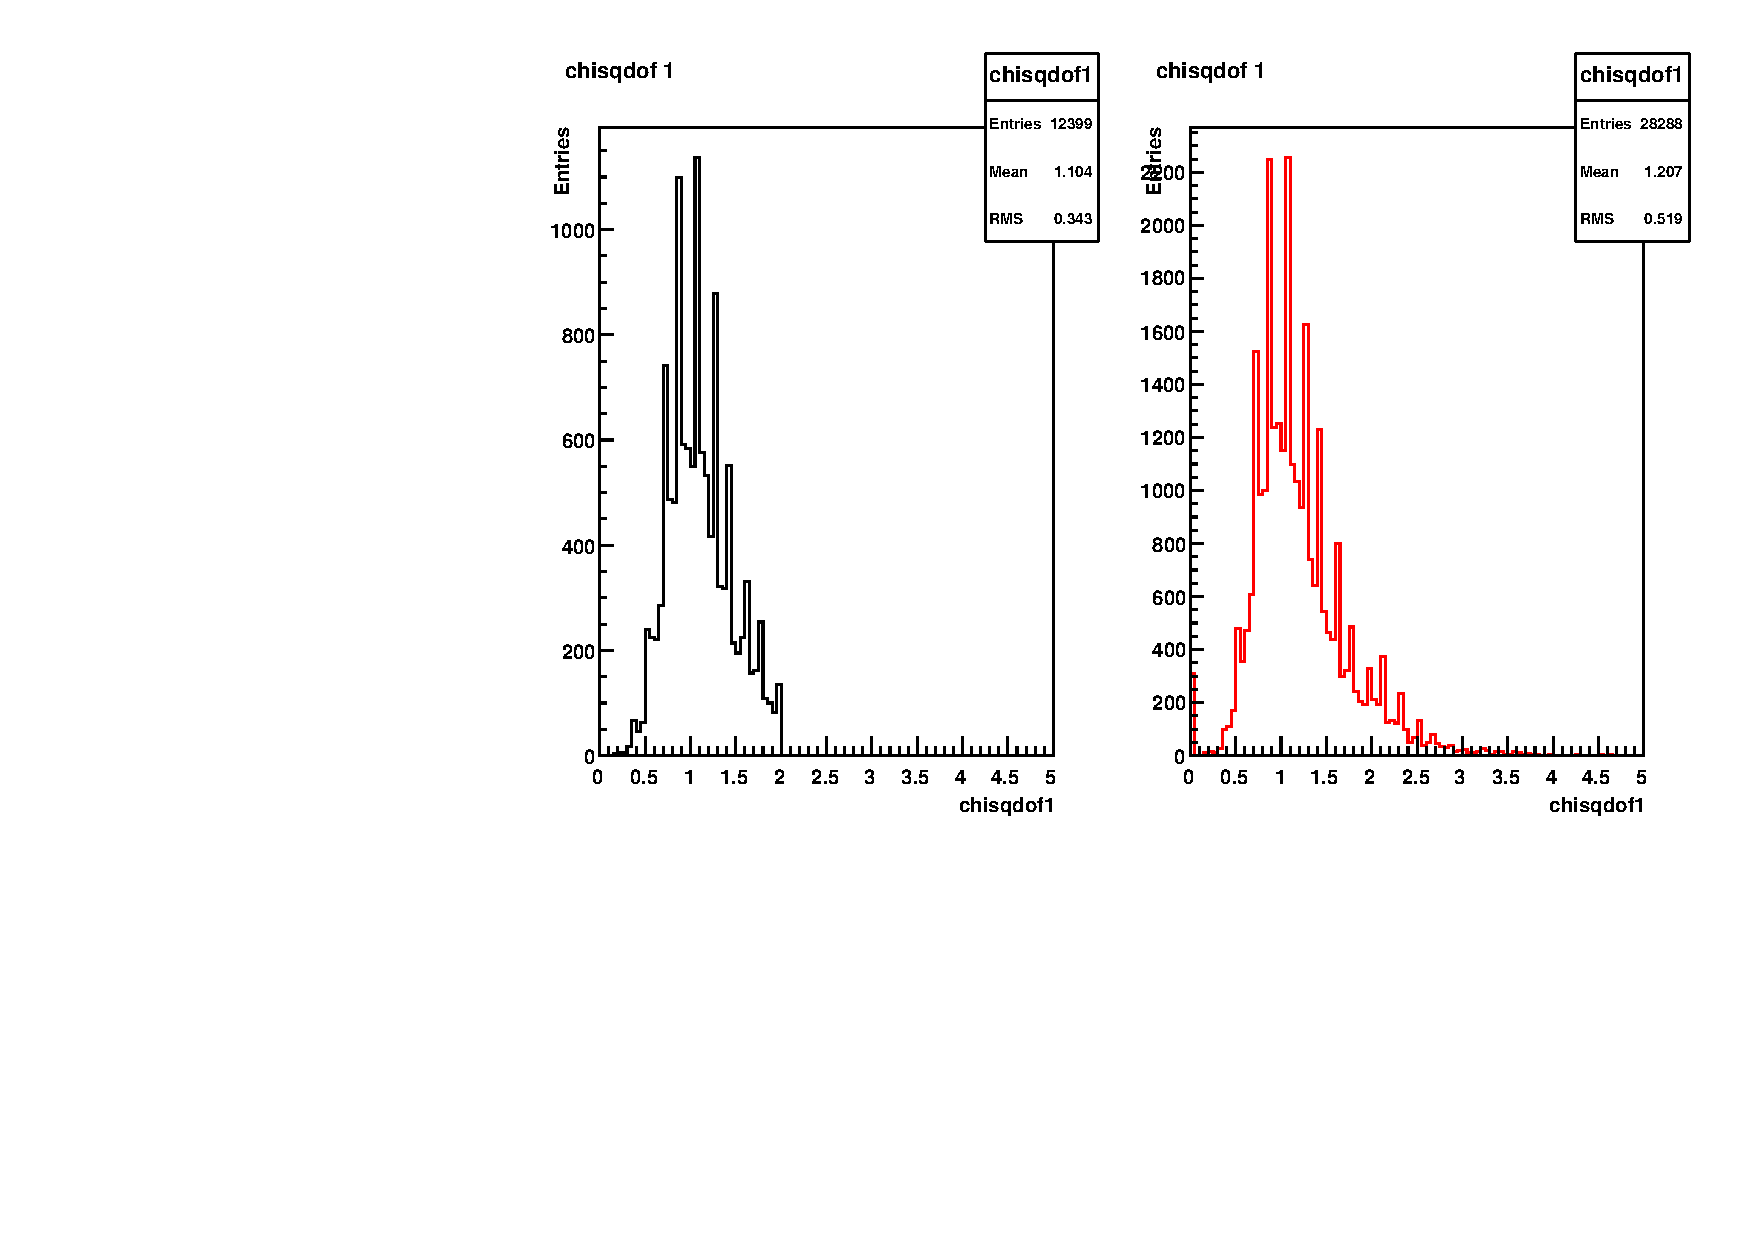
\includegraphics[width=0.45\textwidth]{fig/zmc_cut_chisqdof1.pdf}
        }
        \subfigure[]{
            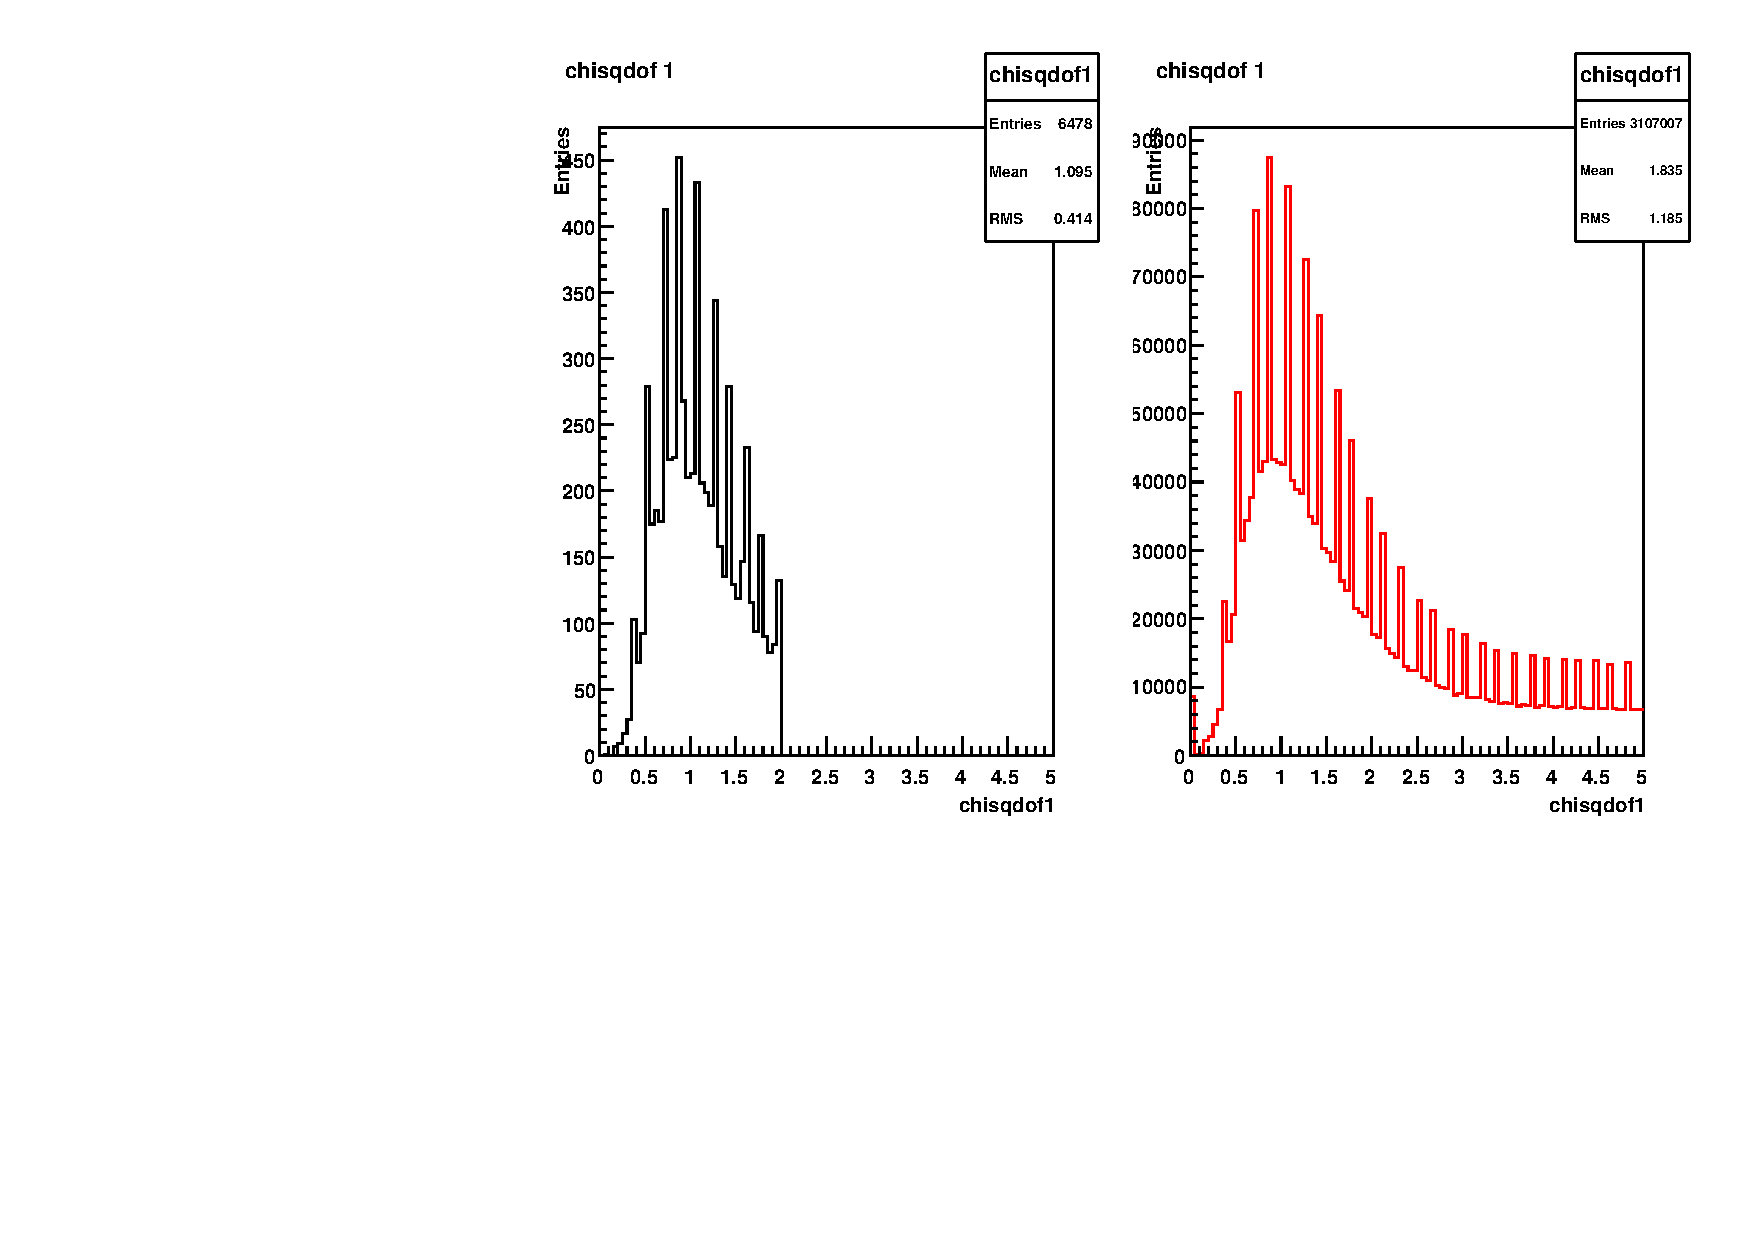
\includegraphics[width=0.45\textwidth]{fig/data_cut_chisqdof1.pdf}
        }\\ %  ------- End of the first row ----------------------%
        \subfigure[]{
            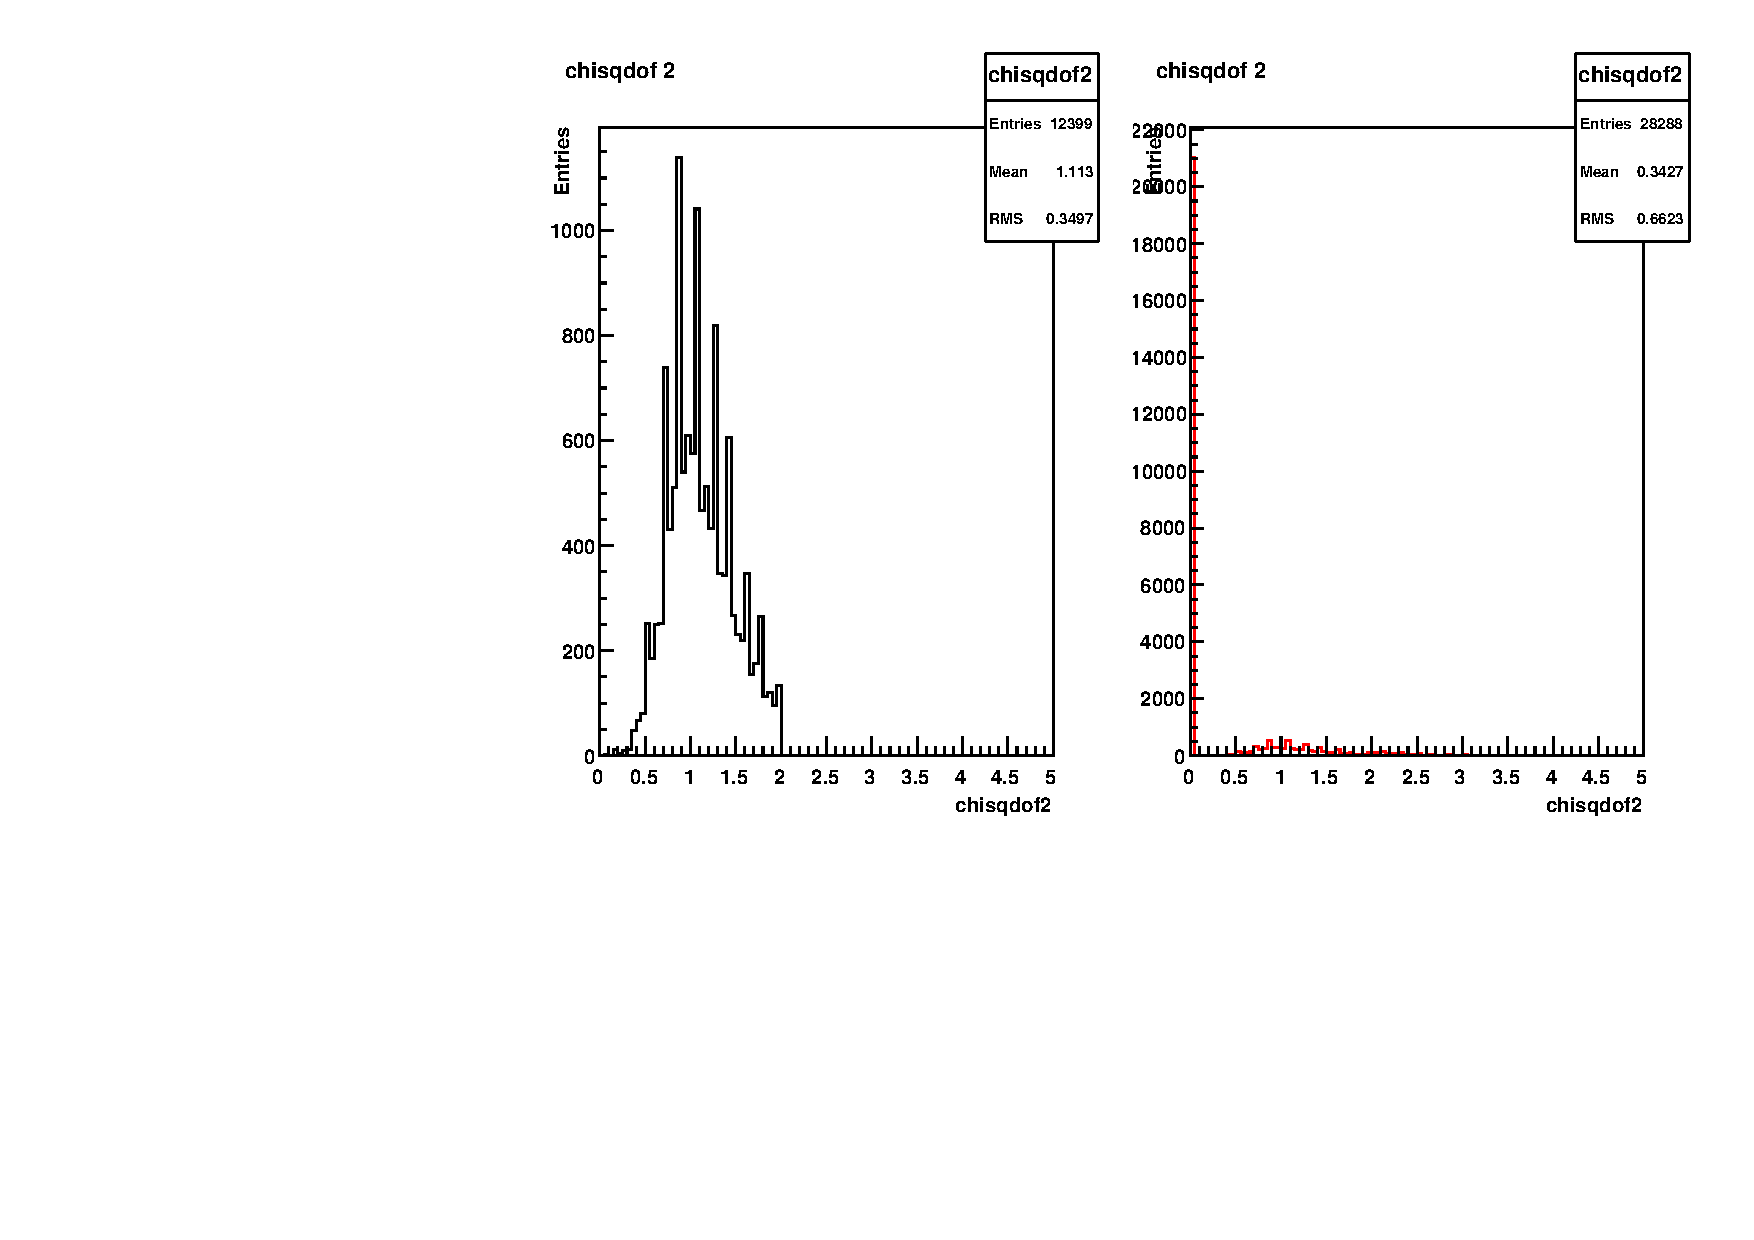
\includegraphics[width=0.45\textwidth]{fig/zmc_cut_chisqdof2.pdf}
        }
        \subfigure[]{
            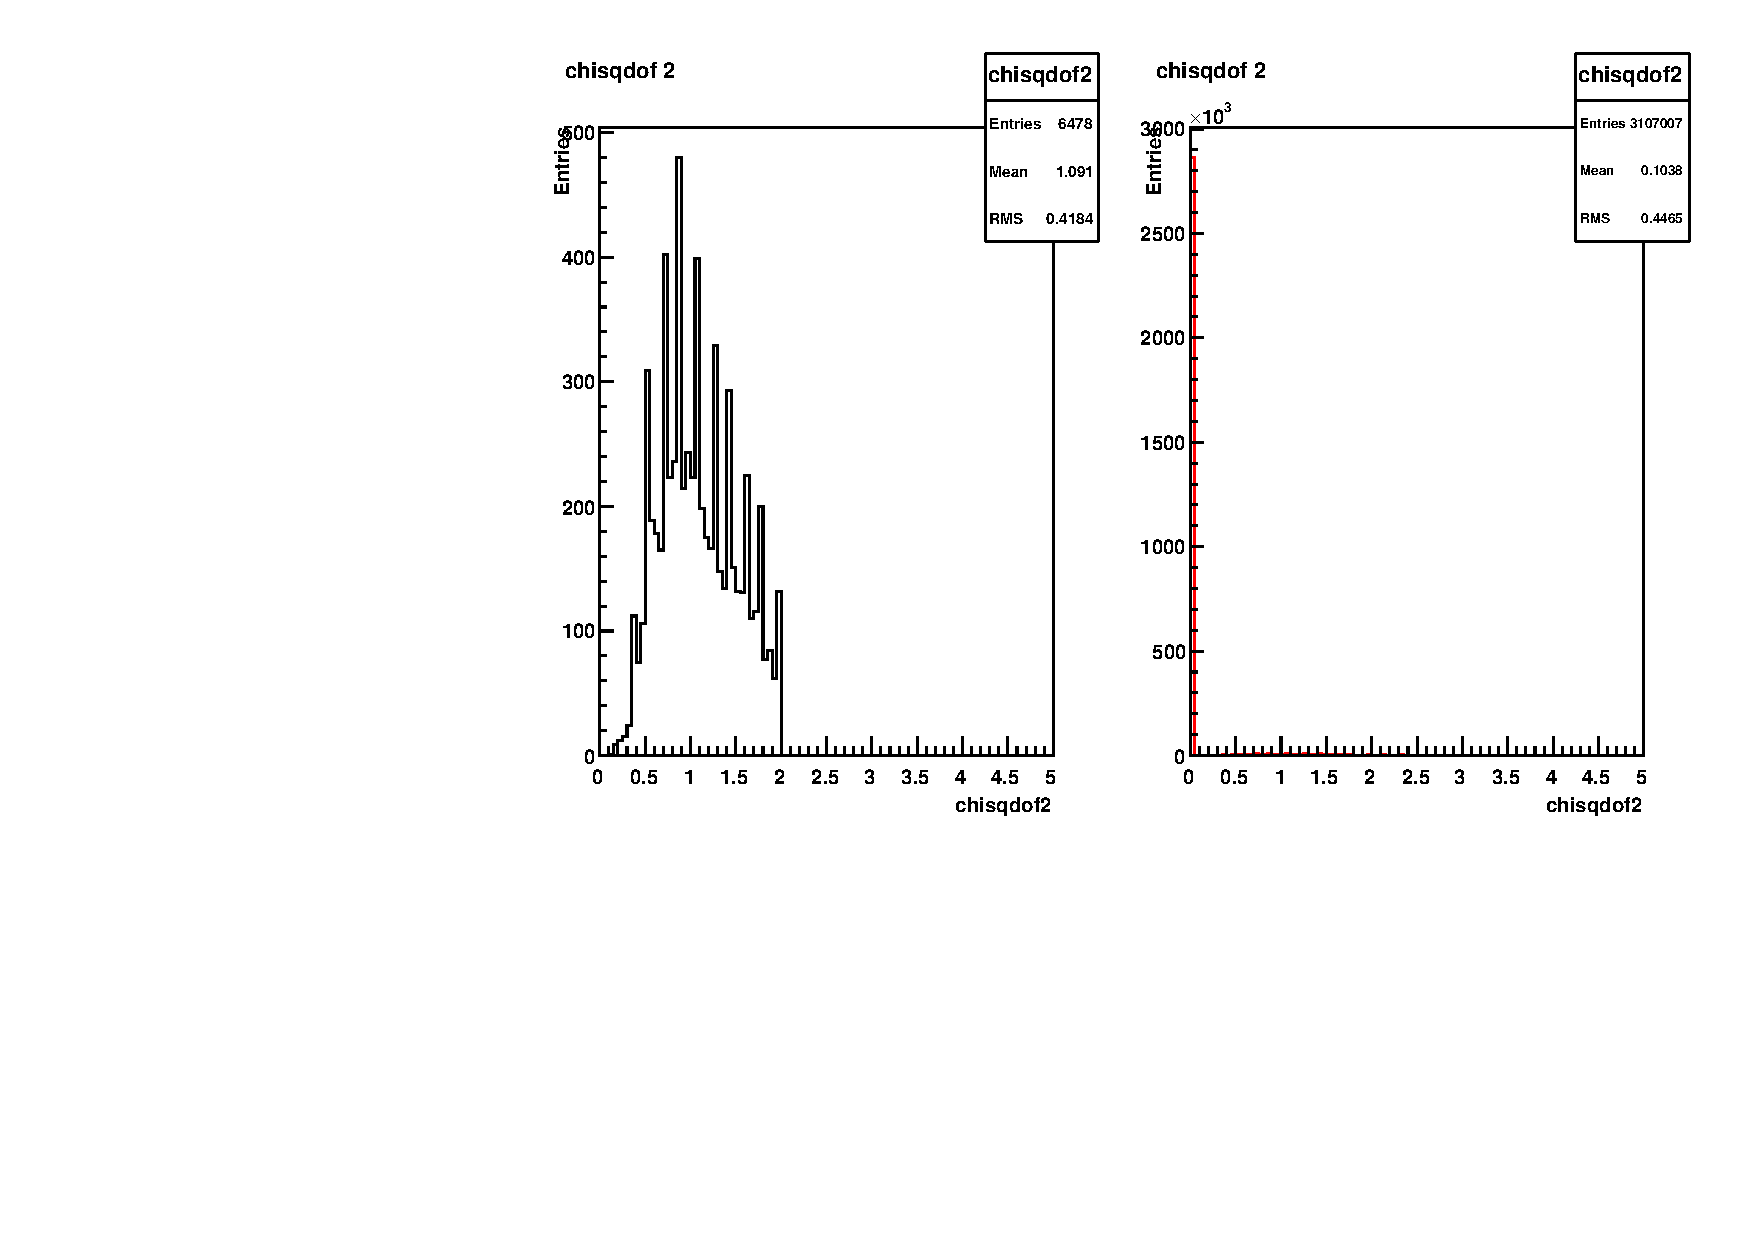
\includegraphics[width=0.45\textwidth]{fig/data_cut_chisqdof2.pdf}
        }
    \end{center}
    \caption{
        $\chi^2$ for accepted (black) and rejected (red) events
            for (a,c): the $Z$ monte-carlo data (b,d): the real data.}{
     }
   \label{fig:chi}
%\end{figure}\bibliography{literatur}
\end{sidewaysfigure}
\begin{sidewaysfigure}
%\begin{figure}[ht!]
     \begin{center}
        \subfigure[]{
            \label{fig:first}
            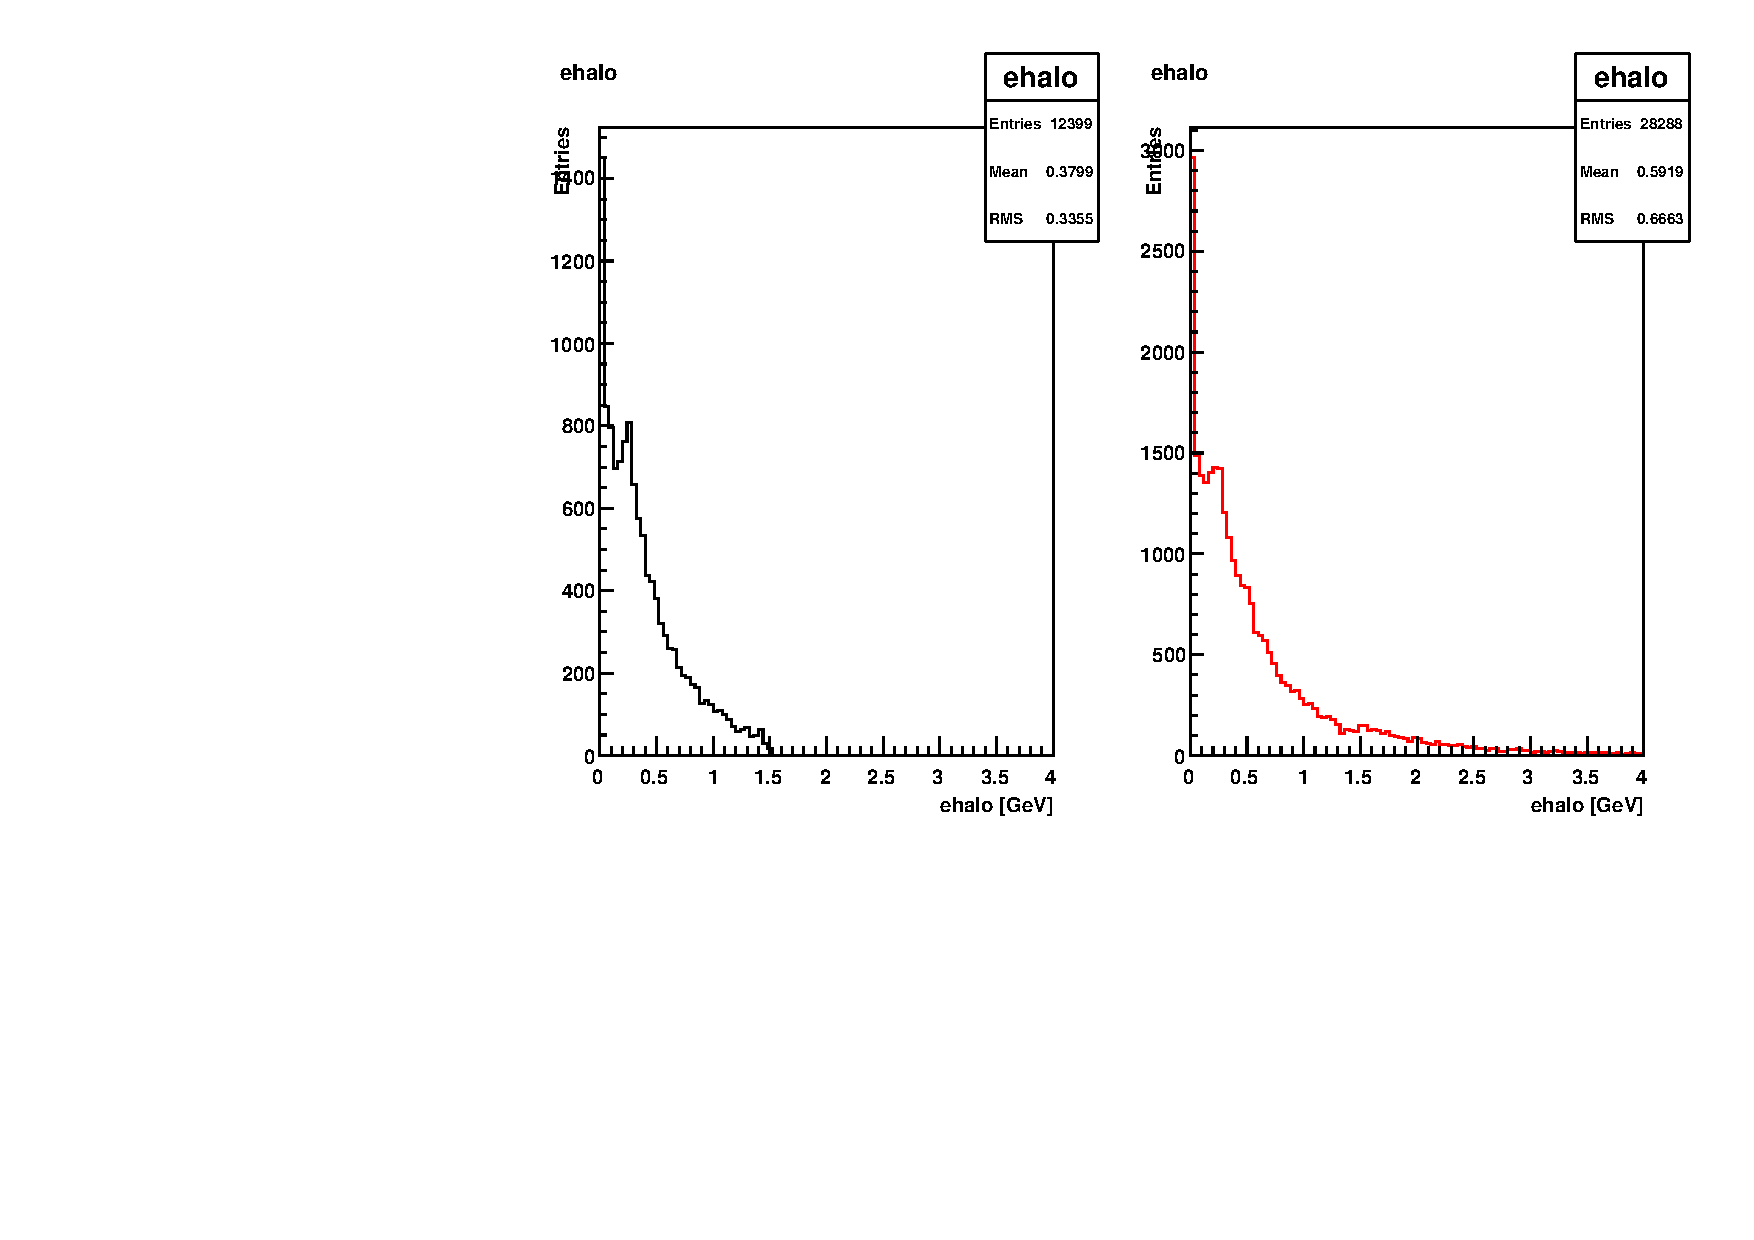
\includegraphics[width=0.45\textwidth]{fig/zmc_cut_ehalo1.pdf}
        }
        \subfigure[]{
           \label{fig:second}
            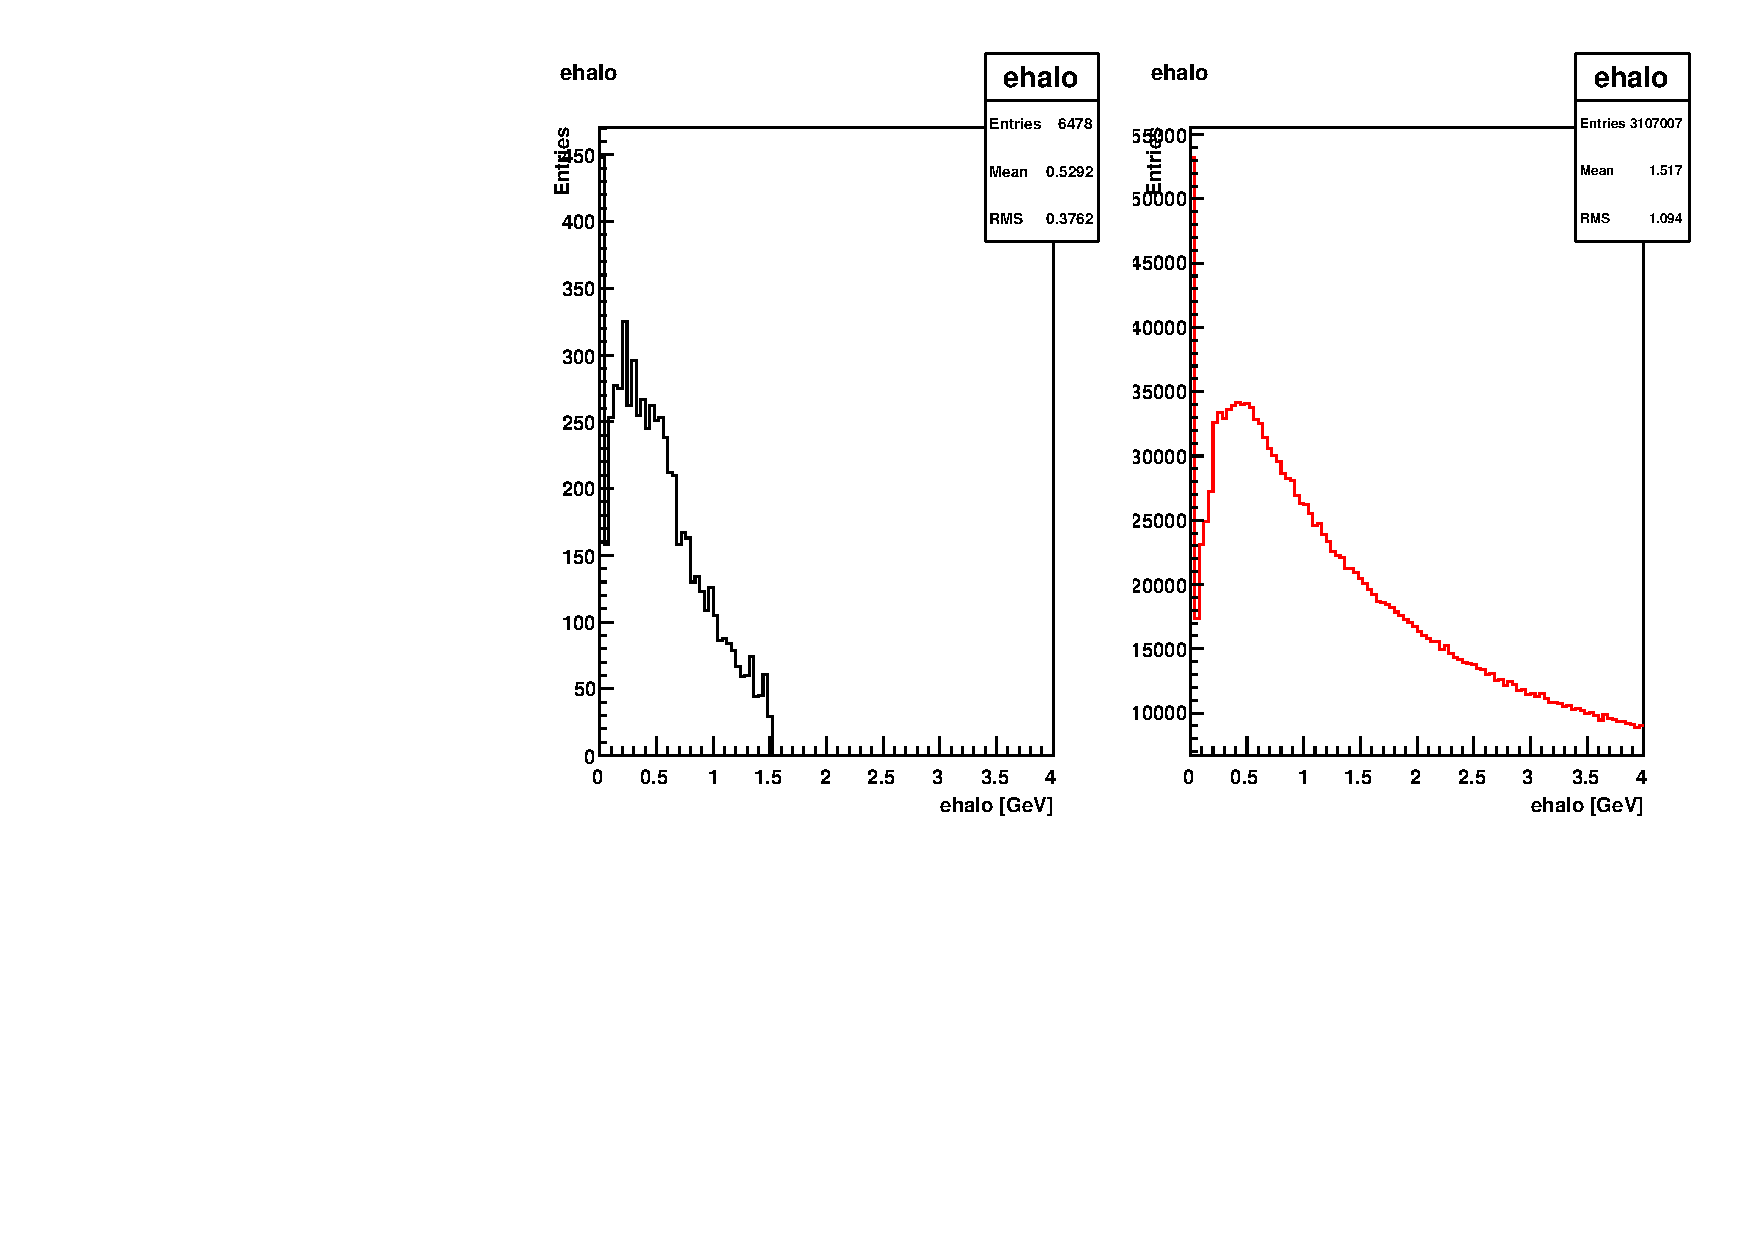
\includegraphics[width=0.45\textwidth]{fig/data_cut_ehalo1.pdf}
        }\\ %  ------- End of the first row ----------------------%
        \subfigure[]{
            \label{fig:third}
            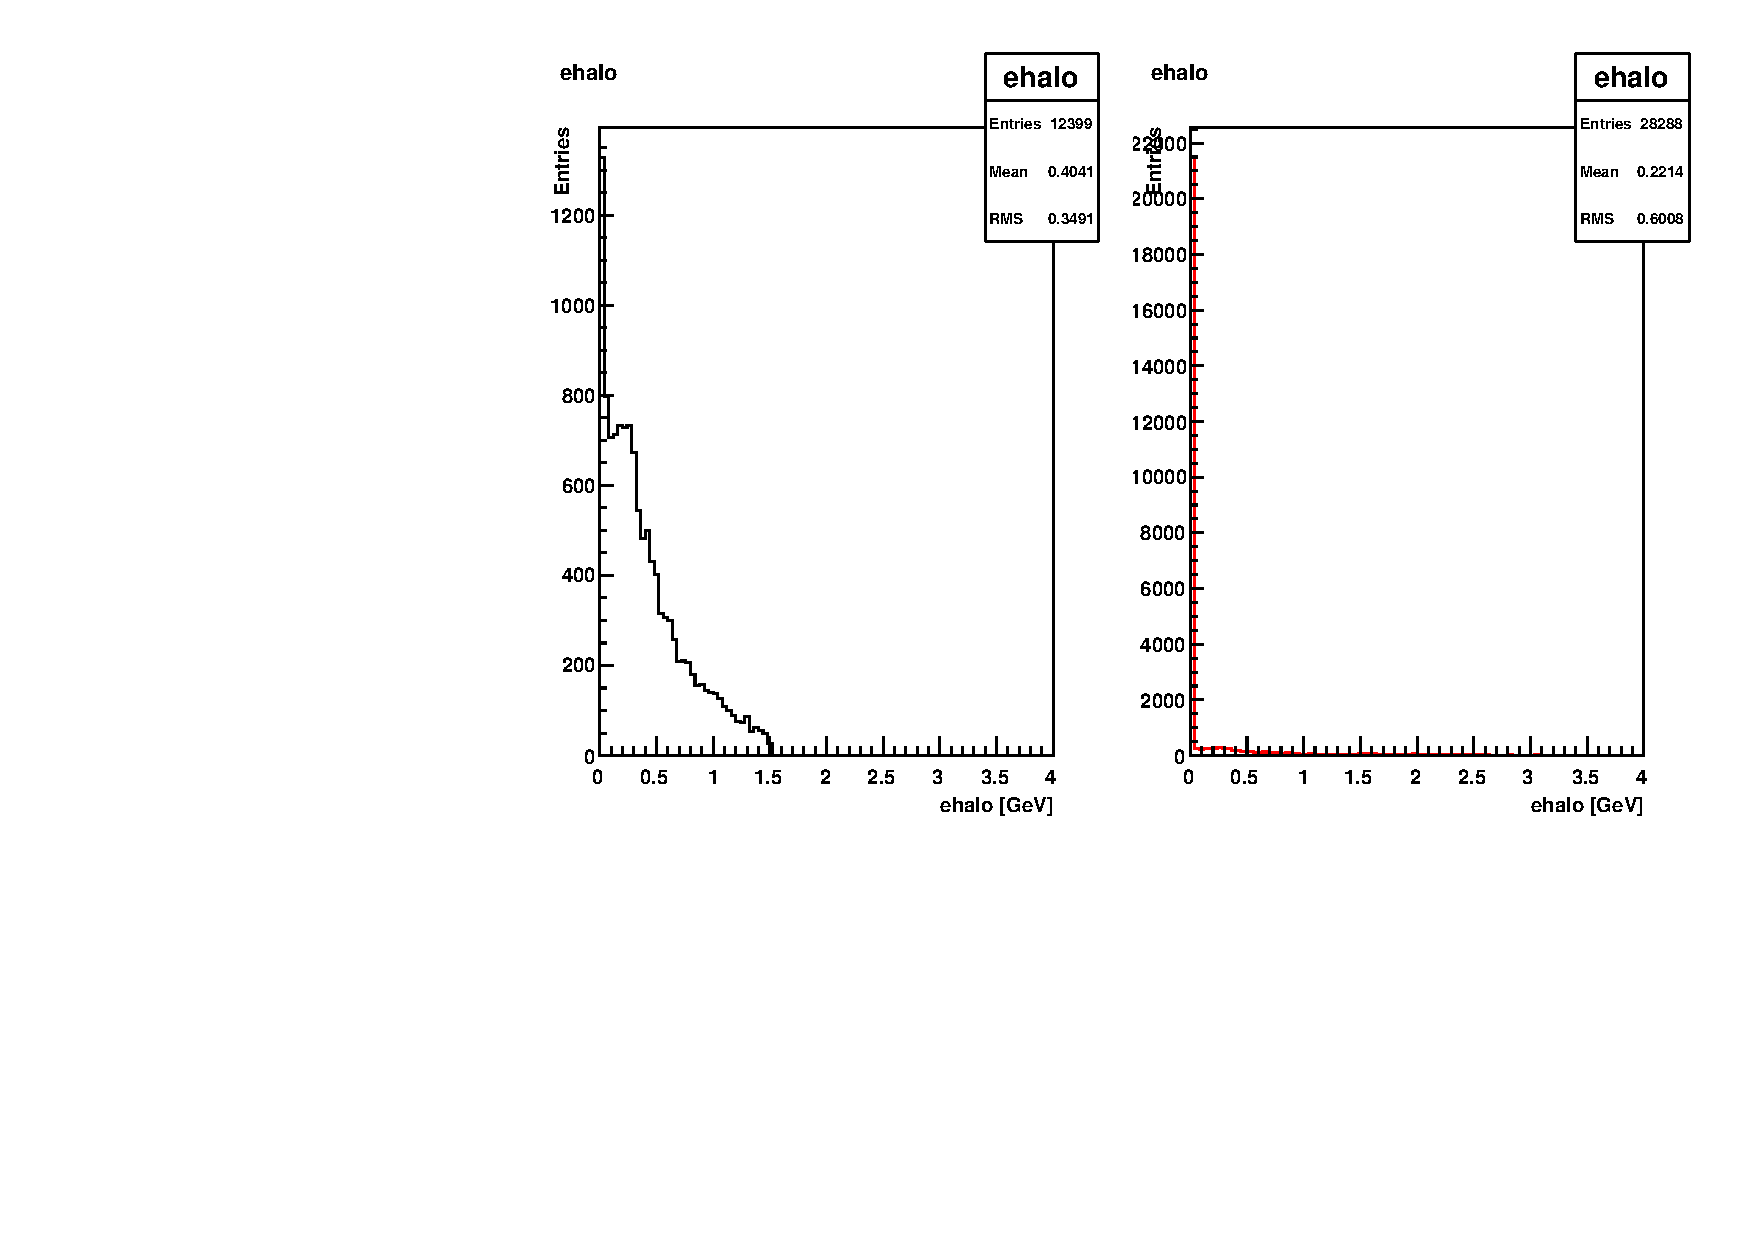
\includegraphics[width=0.45\textwidth]{fig/zmc_cut_ehalo2.pdf}
        }
        \subfigure[]{
            \label{fig:fourth}
            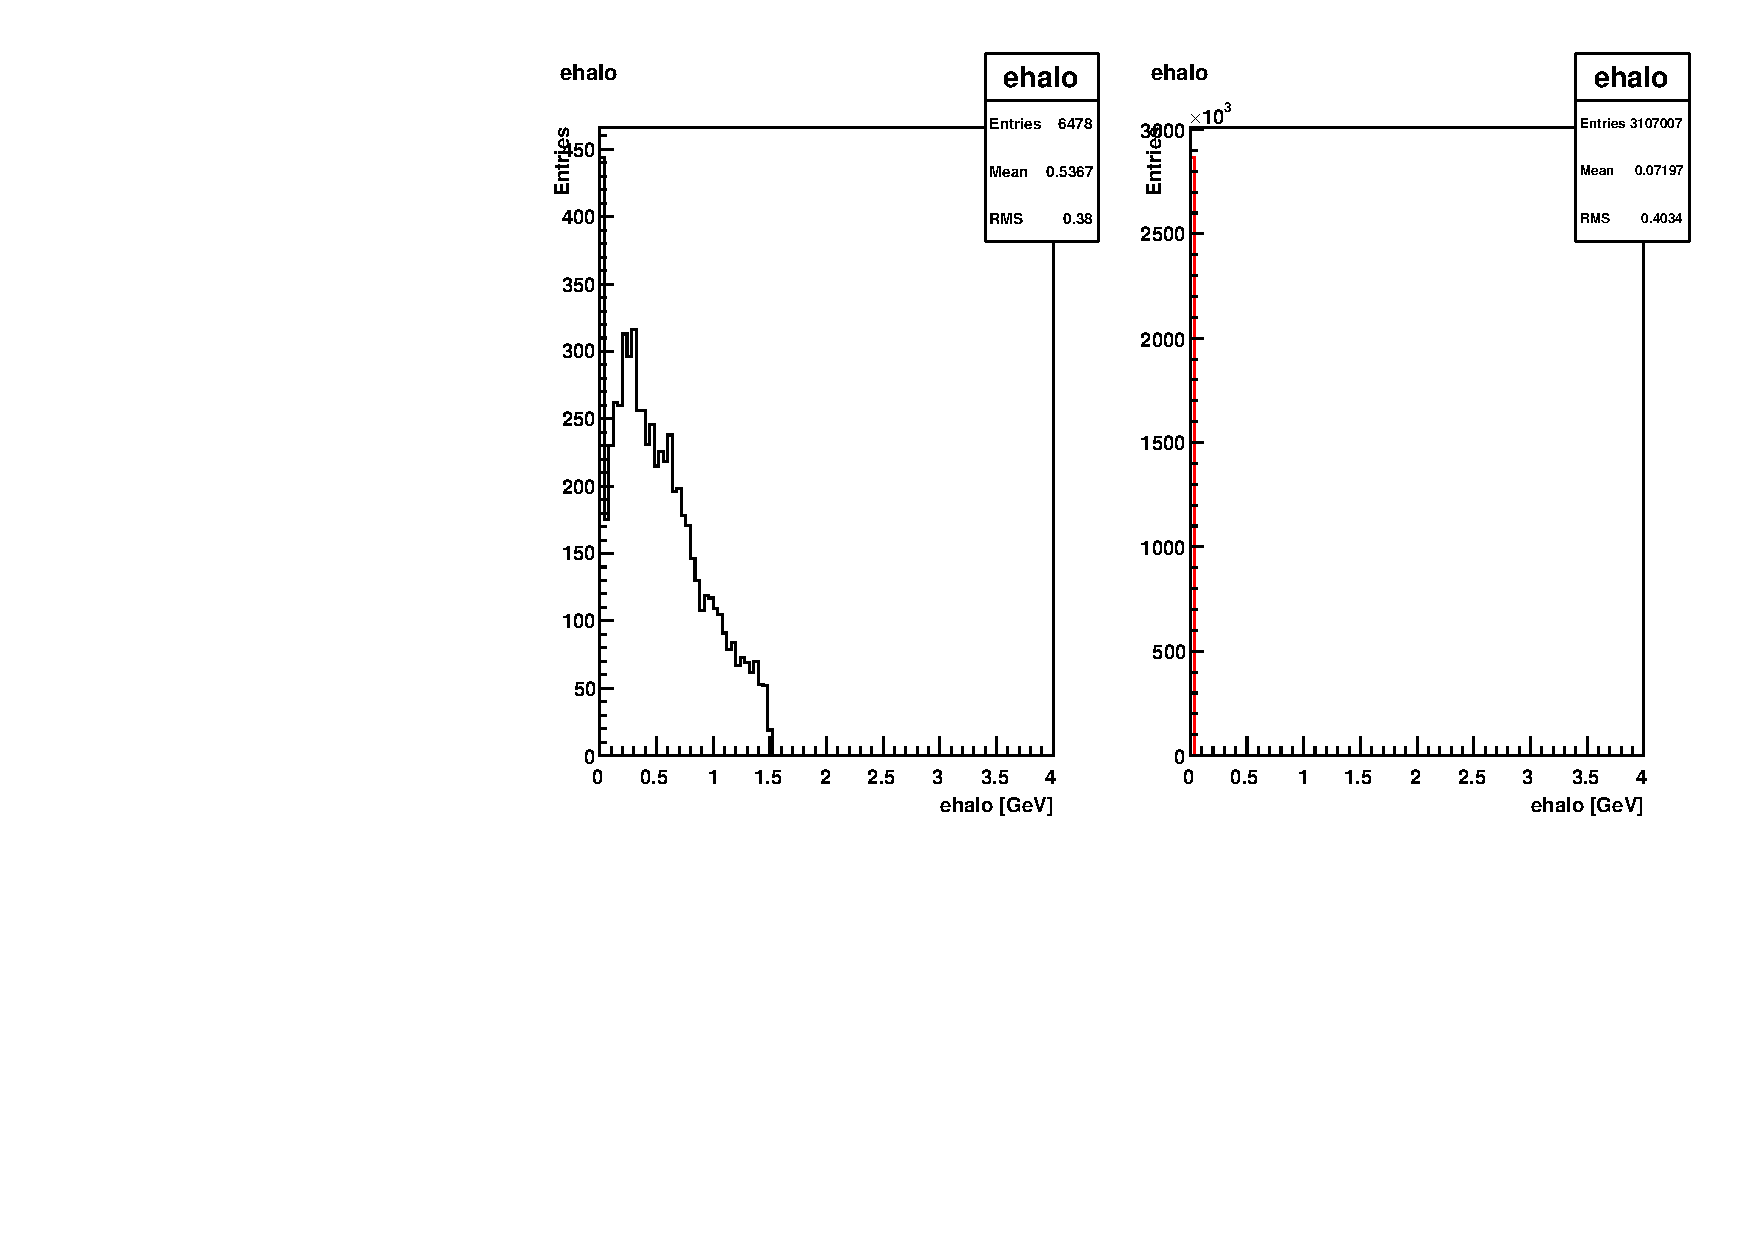
\includegraphics[width=0.45\textwidth]{fig/data_cut_ehalo2.pdf}
        }
    \end{center}
    \caption{
    $E_{\text{halo}}$ for accepted (black) and rejected (red) events
            for (a,c): the $Z$ monte-carlo data (b,d): the real data.}{
     }
  \label{fig:ehalo}

%{()}

%\end{figure}
\end{sidewaysfigure}
\end{appendices}

\end{document}

